
\chapter{核磁共振量子计算}

1938年,Rabi发现处于磁场中的原子核会沿着磁场方向呈正向或反向平行排列,而在施加射频场之后,
这些原子核的自旋方向会发生翻转,这就是著名的拉比振荡(Rabi oscillation) \cite{rabi}。Rabi振荡是人类关于原子核与外加磁场和射频场的相互作用现象的最早认识,而Rabi本人也赢得了1944年的诺贝尔物理奖。1946年,
Bloch和Purcell则发现处于外磁场中的特定核自旋,比如$^1$H, $^{31}$P等,会吸收特定频率的射频场能量,这是人类对于核磁共振最初的认识\cite{nmrhistory},两人也分享了1952年的诺贝尔物理奖。

后来,人们发现核磁共振(Nuclear Magnetic Resonance, 以后均简称为NMR)现象有非常多的应用。在化学上,NMR可以用来解析分子结构,从最早期的简单一维氢谱到后来的$^{13}$C谱,二维谱等高级谱图,NMR可以分析的分子结构
越来越复杂。在化学领域,NMR谱与紫外光谱、红外光谱和质谱并称为“四大名谱”,而我国的高中化学教材里也加入了NMR介绍的章节。除了化学上,医学家们也发现人体中水分子的
氢原子可以产生核磁共振现象,可以通过这一现象获取人体内水分子的分布信息,进而精确绘制人体的内部结构,这也就是目前在医学上广泛应用的核磁共振成像技术(MRI)。

另一方面,超过50年的NMR技术的发展成熟使人们早已可以精确操控NMR中耦合起来的两能级量子系统。在量子计算的概念提出后,NMR也自然的成为非常有潜力的实验验证量子计算
方案的平台,并一直作为各个量子计算潜在方案中操控比特数最多,量子算法最复杂的一个方案而被广泛研究,而在NMR量子计算中发展出的许多技术不仅可以应用在NMR在其他领域的研究上,也
经常被借鉴于其他量子计算平台。在本章中,我们将从NMR如何进行量子计算讲起,包括内部和外部哈密顿量形式,
脉冲技术和逻辑门操作,以及初态制备和测量读出等实现量子计算机的各方面要求。通过这些内容,我们会具体分析NMR量子计算的利弊。而在本章的最后,我们将给出如何利用并不常见的强耦合体系NMR做量子计算,并
给出实验上利用四比特强耦合体系进行143大数分解的实例。

\section{NMR系统}

对于NMR系统最简单的描述就是内部系统哈密顿量与外部控制哈密顿量联合进行动力学演化的过程。系统哈密顿量给出在静磁场中单个的,或者耦合起来的核自旋的能量形式,而控制哈密顿量
则是来自于以系统的共振频率外加的射频脉冲。一般来说,NMR中我们常用的是旋转坐标系,在这个坐标系里考虑问题会相当简单。

\subsection{内部哈密顿量}

在一个沿$\hat{z}$方向的静磁场$B_0$中,自旋1/2的粒子(在本论文中,我们不考虑更高阶的自旋)的动力学演化将被其系统哈密顿量主导
\begin{equation}\label{static}
 H_{0} = -\hbar \gamma B_0 I_z = -\hbar \omega_0 I_z = \left(
                                                         \begin{array}{cc}
                                                           -\hbar \omega_0/2 & 0 \\                                                           0& \hbar \omega_0/2 \\
                                                         \end{array}
                                                       \right),
\end{equation}
其中$\gamma$是原子核的旋磁比,$\omega_0/2 \pi$是Larmor频率,$I_z$是$\hat{z}$方向的核自旋算符。$I_x, I_y, I_z$和Pauli算符有如下的对应形式
\begin{equation}\label{static}
 \sigma_x = 2I_x,  \sigma_y = 2I_y,  \sigma_z = 2I_z ,
\end{equation}
并且
\begin{equation}\label{static}
 \sigma_x \equiv \left(
                   \begin{array}{cc}
                     0 & 1 \\
                     1 & 0 \\
                   \end{array}
                 \right);
  \sigma_y \equiv \left(
                   \begin{array}{cc}
                     0 & -i \\
                     i & 0 \\
                   \end{array}
                 \right);  \sigma_z \equiv \left(
                   \begin{array}{cc}
                     1 & 0 \\
                     0 & -1 \\
                   \end{array}
                 \right).
\end{equation}

对于这种系统哈密顿量的形式更直观的理解是,本征态$\left\vert  0 \right\rangle$(有时候也叫$\left\vert  \uparrow \right\rangle$)的能量本征值将比
本征态 $\left\vert  1 \right\rangle$(有时候也叫$\left\vert  \downarrow \right\rangle$) 小$\hbar \omega_0$,这种能量劈裂叫做Zeeman劈裂。

\begin{figure}[htbp]
            \begin{center}
              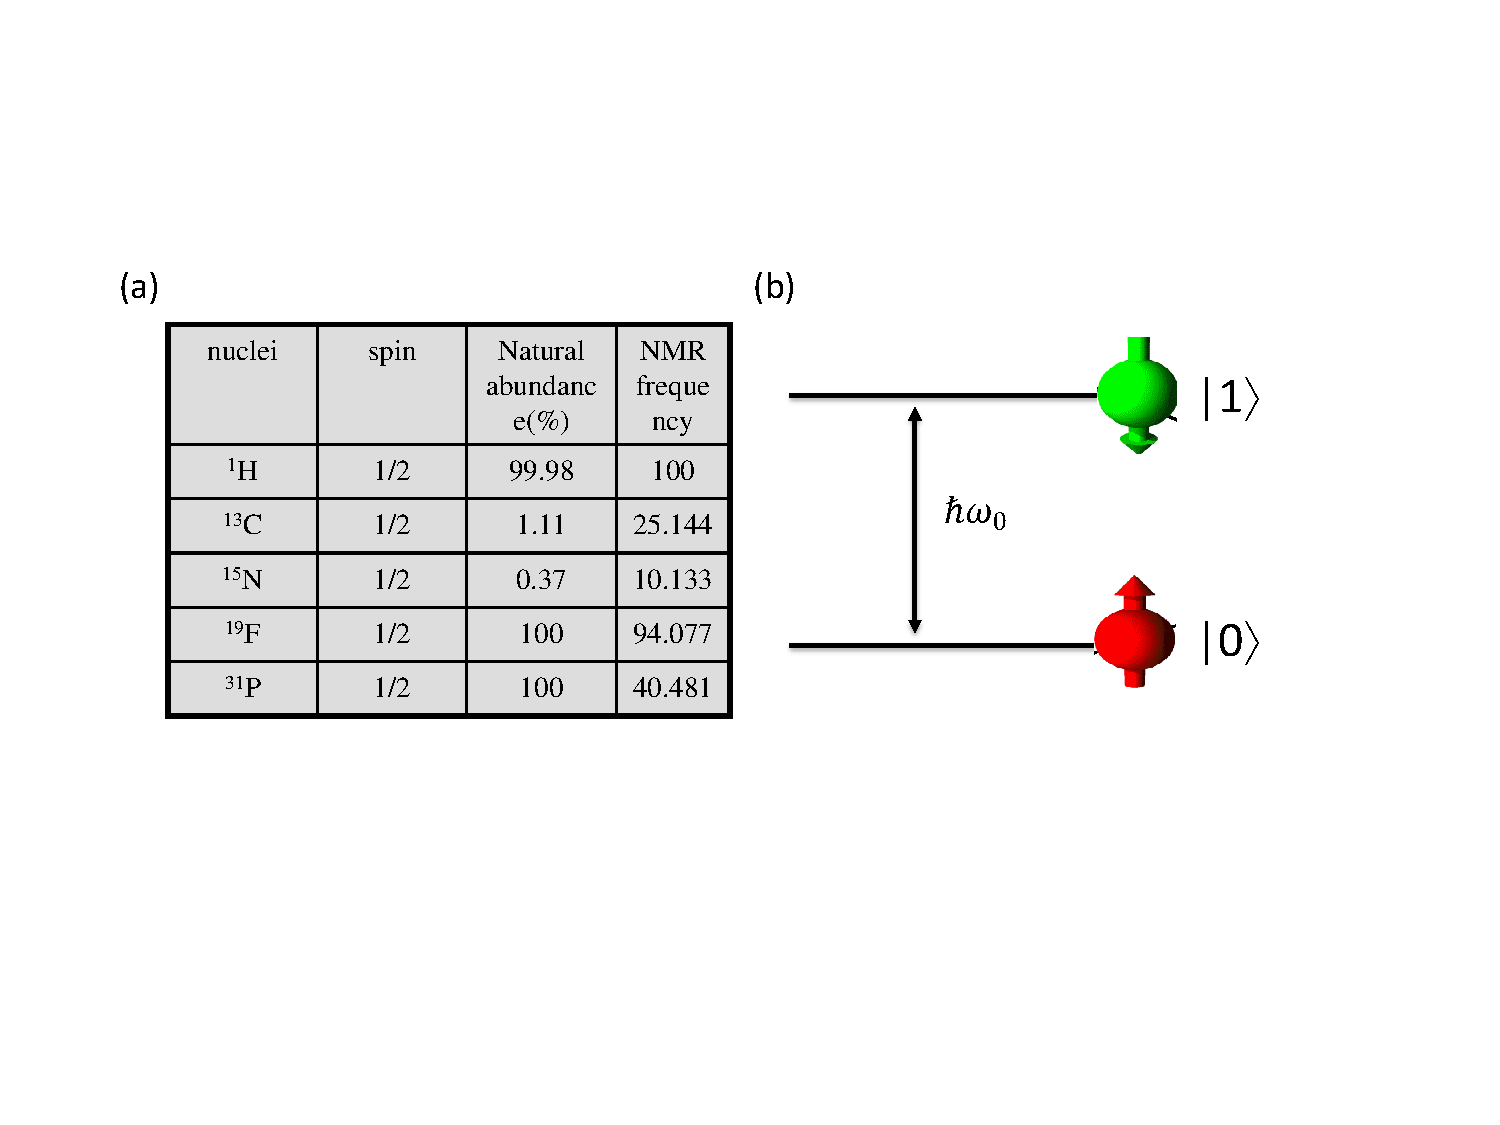
\includegraphics[width= 0.8\columnwidth]{figures/spinhalf.pdf}
              \caption{(a) 几种常用的自旋1/2粒子的天然丰度及Larmor频率。(b) 自旋 1/2粒子的能级图。
              }
              \label{spinhalf}
            \end{center}
\end{figure}

我们可以近似地把时间演化算子$U=e^{-iHt}$理解为一个矢量在Bloch球上绕着$\overrightarrow{B_0}$的进动过程。方便起见,我们把Bloch球的$\hat{z}$轴定义为$\overrightarrow{B_0}$
方向,而$\left\vert  0 \right\rangle$沿着$+\hat{z}$方向,$\left\vert  1 \right\rangle$沿着$-\hat{z}$方向。对于液体NMR的情况来说,$B_0$的典型值为5-15T,导致进动频率$\omega_0$的大小为几百MHz,也就是射频的范围。

不同种类的核自旋可以很容易地辨别,因为它们的旋磁比$\gamma$不同,从而拥有相差很远的Larmor频率。对于相同的原子核来说,它们也有不同的频率,叫做化学位移。化学位移来源于环绕原子核周围的电子云产生的磁场的部分屏蔽作用,该屏蔽的大小取决于原子核周围的电子分布,因此具有不同核外电子环境的原子核
具有不同的化学位移。典型的化学位移范围依赖于不同的原子核,比如对$^1$H来说,它的范围约为10ppm(百万分之一,NMR常用的频率单位),对$^{13}$C和
$^{19}$F则约为200ppm。在静磁场$B_0$的大小为10T时,化学位移的值大概从几kHz到数十kHz,相比于Larmor频率的百万MHz的数量级来说还是非常小的。

一般来说,化学位移是空间各向异性的,要用张量来描述。在液体NMR中,由于分子间的快速滚动,各向异性的影响被平均掉了,而在固体NMR中,
各向异性表明化学位移是依赖于分子取向的,也就是和静磁场$B_0$的夹角。

不同于孤立的原子核的哈密顿量,有相互作用的原子核主要存在两种不用的相互作用机制:直接的偶极-偶极耦合以及间接的标量耦合。

(a) \emph{直接耦合}

偶极-偶极耦合的相互作用类似于两个临近的条形磁体的相互作用,它纯粹是通过空间产生相互作用的,并不需要第三方介质。该作用主要依赖于
核间矢量$\overrightarrow{r_{ij}}$,可以被如下哈密顿量形式描述
\begin{equation}\label{static}
H_D = \sum_{i<j} \frac{\mu_0\gamma_i \gamma_j \hbar}{4\pi |\overrightarrow{r_{ij}}|^3}(\overrightarrow{I^i}\cdot \overrightarrow{I^j}-\frac{3}{|\overrightarrow{r_{ij}}|^2(\overrightarrow{I^i}\cdot\overrightarrow{r_{ij}})(\overrightarrow{I^j}\cdot\overrightarrow{r_{ij}})}),
\end{equation}
其中$\overrightarrow{I_{i}}$自旋$i$的磁化矢量。在高场情况下,该耦合形式可以近似为
\begin{equation}\label{static}
H_D = \sum_{i<j} \frac{\mu_0\gamma_i \gamma_j \hbar}{8\pi |\overrightarrow{r_{ij}}|^3}(1-3cos^2\theta_{ij})(3I_z^i I_z^j-\overrightarrow{I^i}\cdot\overrightarrow{I^j}),
\end{equation}
$\theta_{ij}$是$B_0$和$\overrightarrow{r_{ij}}$的夹角。当化学位移之差$|\omega_0^i-\omega_0^j|$比耦合强度大很多时,
耦合项中的横向分量可以被忽略掉,$H_D$可以进一步被简化为
\begin{equation}\label{static}
H_D = \sum_{i<j} \frac{\mu_0\gamma_i \gamma_j \hbar}{8\pi |\overrightarrow{r_{ij}}|^3}(1-3cos^2\theta_{ij})I_z^i I_z^j.
\end{equation}
这个形式和下面介绍的标量耦合形式类似。

在液体NMR中,不论是分子间的偶极耦合或者分子内部的偶极耦合,由于分子的快速滚动都已经
被平均掉了。而在固体NMR中,我们可以通过施加多脉冲序列\cite{Haeberlen}或者魔角旋转技术实现类似的
简单哈密顿量形式。

(b) \emph{间接耦合}

分子中核自旋的第二种相互作用机制就是$J$耦合,或者叫标量耦合。这种相互作用机制
来源于原子间化学键中的共享电子,或者电子波函数的交叠产生的费米接触相互作用,其大小依赖于相互作用的
原子核种类,并随着化学键数目的增多而减少。典型的$J$耦合强度从几个Hz(三键或四键耦合)到几百Hz(单键耦合)不等。
$J$耦合的哈密顿量形式为
\begin{equation}\label{static}
H_J = \hbar\sum_{i<j} 2\pi J_{ij} \overrightarrow{I^i}\cdot\overrightarrow{I^j}=\hbar\sum_{i<j} 2\pi J_{ij}(I_x^iI_x^j+I_y^iI_y^j+I_z^iI_z^j),
\end{equation}
$J_{ij}$是自旋$i$和自旋$j$之间的相互作用强度。和偶极耦合的形式类似,在弱耦合近似($|\omega_0^i-\omega_0^j|\gg 2\pi |J_{ij}|$)的情况下,该形式可以化简为
\begin{equation}\label{Jappro}
H_J =\hbar\sum_{i<j} 2\pi J_{ij}I_z^iI_z^j.
\end{equation}
对于不同种类的核自旋该条件是容易满足的,而对于很多分子内的同种核自旋该条件也可能满足。

在弱耦合近似下,标量耦合作用可以用有效磁场的概念来理解:除了外加的静磁场$\overrightarrow{B_0}$外,核自旋还会感受到由邻近自旋产生的沿$\pm\hat{z}$方向的磁场。如下图所示,这个附加磁场
会使能级产生移动。当自旋$j$处于$\left\vert  0 \right\rangle$时,自旋$i$的Larmor频率将移动$-J_{ij}/2$;当自旋$j$处于$\left\vert  1\right\rangle$时,自旋$i$的Larmor频率将移动$J_{ij}/2$。

\begin{figure}[htbp]
            \begin{center}
              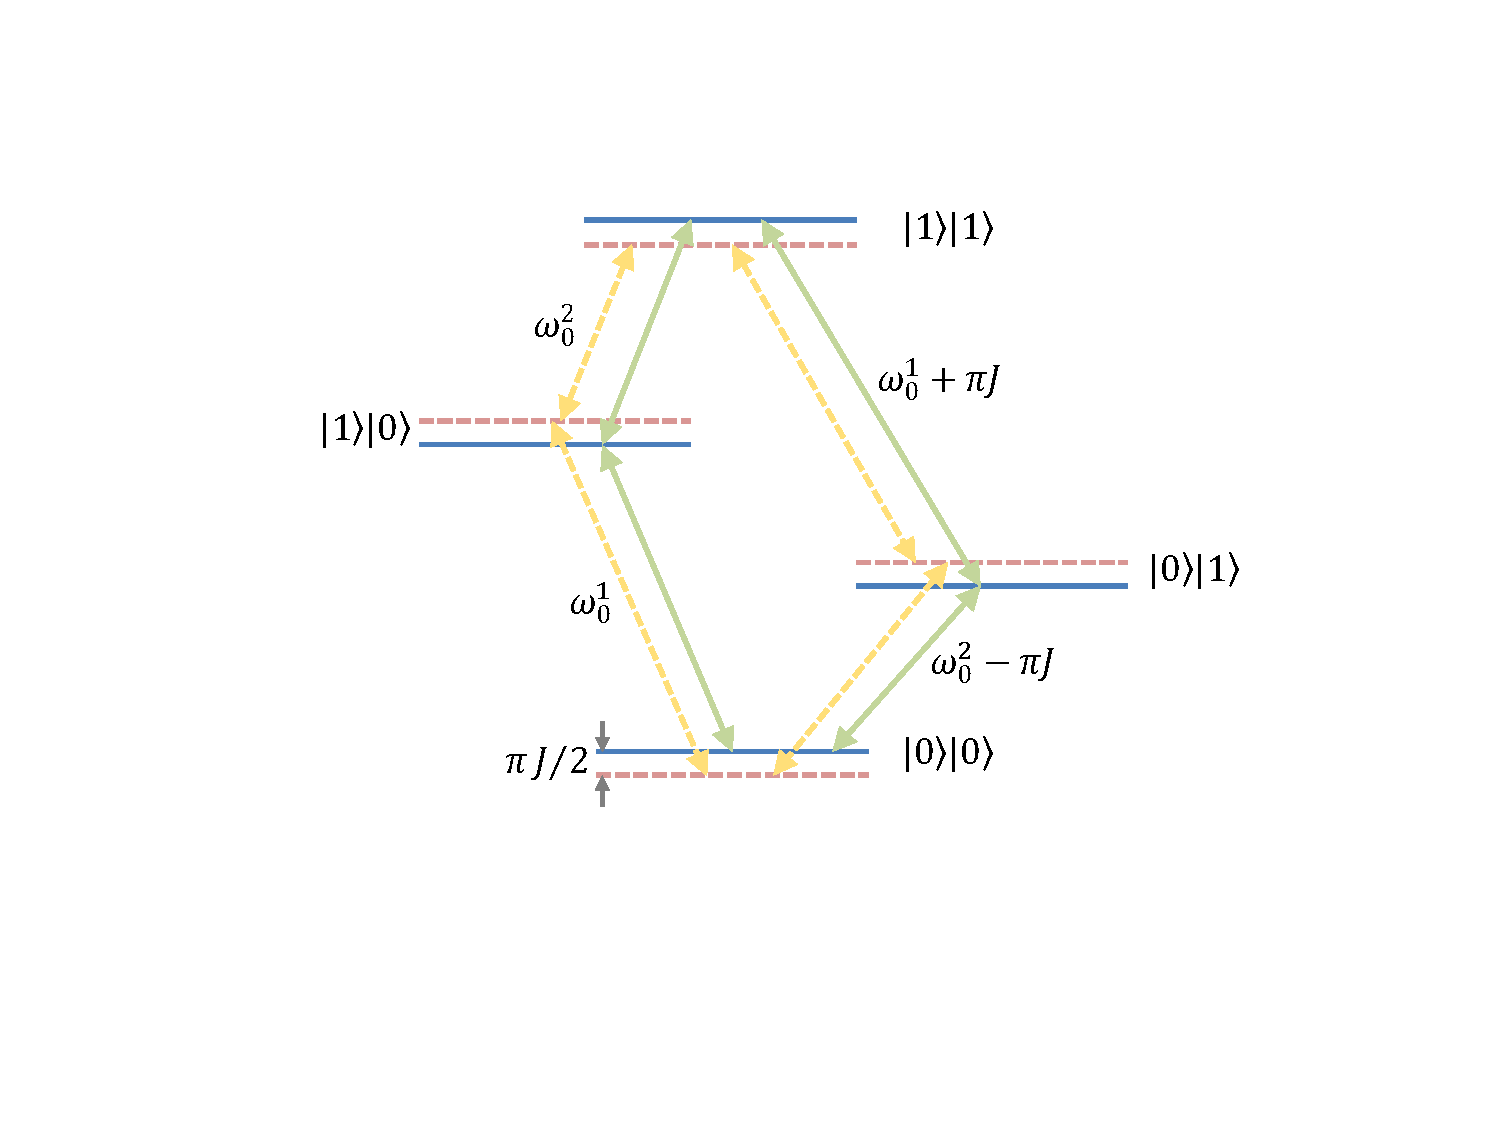
\includegraphics[width= 0.8\columnwidth]{figures/energy.pdf}
              \caption{两个未耦合的自旋的能级图(虚线)及以式\ref{Jappro}形式耦合的哈密顿量的能级图(实线)。$\hbar$已经被忽略掉。
              }
              \label{energy}
            \end{center}
\end{figure}

对于耦合起来的两个自旋系统来说,自旋$i$的频率谱线包含分离的两条,它们之间的距离为$J_{ij}$,且其中心频率
为$\omega_0^i$。两条谱线是对应于自旋$j$所处的状态的。相应地,对于三个两两耦合的自旋来说,每个自旋将
包含四条谱线,而每添加一个自旋,谱线的数目将翻倍。

所有两两耦合的大小可以通过读出不同自旋的谱线劈裂来得到。$J$耦合的符号则可以用适当的
核选脉冲序列,例如二维COSY实验\cite{sign1}或者线选脉冲的连续激发来检测。注意仅仅通过简单的NMR谱线来确定$J$耦合的符号
是不可能的。

综上所述,对于$n$个两两耦合的自旋系统来说,其最简单的哈密顿量形式为
\begin{equation}\label{aaa}
H_{sys} =-\hbar\sum_{i}\omega_0^i I_z^i+ \hbar\sum_{i<j} 2\pi J_{ij}I_z^iI_z^j.
\end{equation}
在绝大多数的NMR量子计算实验中用到的自旋系统都可以用这个哈密顿量形式来描述。

\subsection{外部哈密顿量}

本小节我们转到如何操控NMR系统上。对处于$\hat{z}$方向静磁场中的自旋1/2粒子来说,我们可以通过
外加电磁场$\overrightarrow{B_1}(t)$来进行操控。该电磁场可以加在$\hat{x}-\hat{y}$平面内的任意角度,其频率为$\omega_{rf}$,该频率的大小处于或接近自旋
的进动频率$\omega_0$。对于处于射频场中的单自旋来说,其哈密顿量形式为
\begin{equation}\label{aaa}
H_{rf} =-\hbar\gamma B_1 [cos(\omega_{rf}t+\phi)I_x-sin(\omega_{rf}t+\phi)I_y],
\end{equation}
其中$B_1$和$\phi$分别是射频场的强度和相位。射频场强度$\omega_1=\gamma B_1$的典型值为液体NMR中的小于30kHz,固体NMR中几百kHz。

对于$n$个自旋,射频场的哈密顿量为
\begin{equation}\label{aaa}
H_{rf} =-\sum_i^n\hbar\gamma_i B_1 [cos(\omega_{rf}t+\phi)I_x^i-sin(\omega_{rf}t+\phi)I_y^i].
\end{equation}
一般来说,在实验室坐标系中,外磁场在固定的、和静磁场垂直的轴上振荡。这个振荡可以分解为两部分反方向旋转的磁场:一个使自旋
在其进动方向上以频率$\omega_{rf}$旋转,因此可以将旋转频率设在核自旋的共振频率附近;另一部分则与自旋的进动方向相反,因此距离其共振频率相当远,大概为$2\omega_0$。这部分唯一的影响是Larmor频率上的一个
几乎可以忽略的漂移,称为Bloch-Siegert漂移\cite{bshift}。

注意到与系统中不可控的Larmor进动和耦合项不同,外加射频场的强度$B_1$和相位$\phi$都可以随时间改变而加以控制。我们很快就会看到,正是对于射频场的强度,相位及频率的控制形成了
NMR量子计算的核心。

在常用的实验室坐标系中,由于要同时考虑静磁场和旋转磁场的机制,这时的NMR系统处理起来会相当复杂。如果我们引入一个绕$\hat{z}$轴以$\omega_{rf}$的频率旋转的坐标系,那么这个问题将大大简化。旋转坐标系的一般形式为
\begin{equation}\label{aaa}
\left\vert  \psi \right\rangle^{rot} =e^{-i\omega_{rf}tI_z}\left\vert  \psi \right\rangle.
\end{equation}
把$\left\vert  \psi \right\rangle$的形式代入薛定谔方程
\begin{equation}\label{aaa}
i\hbar(\frac{d\left\vert  \psi \right\rangle}{dt})=H\left\vert  \psi \right\rangle,
\end{equation}
其中哈密顿量为
\begin{equation}\label{aaa}
H = -\hbar \omega_0 I_z -\hbar\omega_1 [cos(\omega_{rf}t+\phi)I_x-sin(\omega_{rf}t+\phi)I_y],
\end{equation}
我们可以得到
\begin{equation}\label{aaa}
i\hbar(\frac{d\left\vert  \psi \right\rangle^{rot}}{dt})=H^{rot}\left\vert  \psi \right\rangle^{rot},
\end{equation}
其中
\begin{equation}\label{aaa}
H^{rot} = -\hbar (\omega_0-\omega_{rf}) I_z -\hbar\omega_1 [cos\phi I_x-sin\phi I_y].
\end{equation}
特别地,如果我们取$\omega_{rf}=\omega_0$,上式中的第一项也将消掉。对于旋转坐标系中
的观察者来说,他将看到自旋只是简单的绕着$\overrightarrow{B_1}$轴进动,这种现象叫做章动(nutation),并且章动的轴由相位$\phi$控制。

如果射频场与核自旋的频率是偏共振的话,假设为$\Delta\omega = \omega_0-\omega_{rf}$,那么旋转坐标系中的自旋将沿一个与$\hat{z}$轴夹角为$\alpha$的轴进动
 \begin{equation}\label{aaa}
\alpha = arctan(\omega_1/\Delta\omega),
\end{equation}
并且其频率为
\begin{equation}\label{aaa}
\omega'_1 = \sqrt{\Delta\omega^2+\omega_1^2}.
\end{equation}

\begin{figure}[htbp]
            \begin{center}
              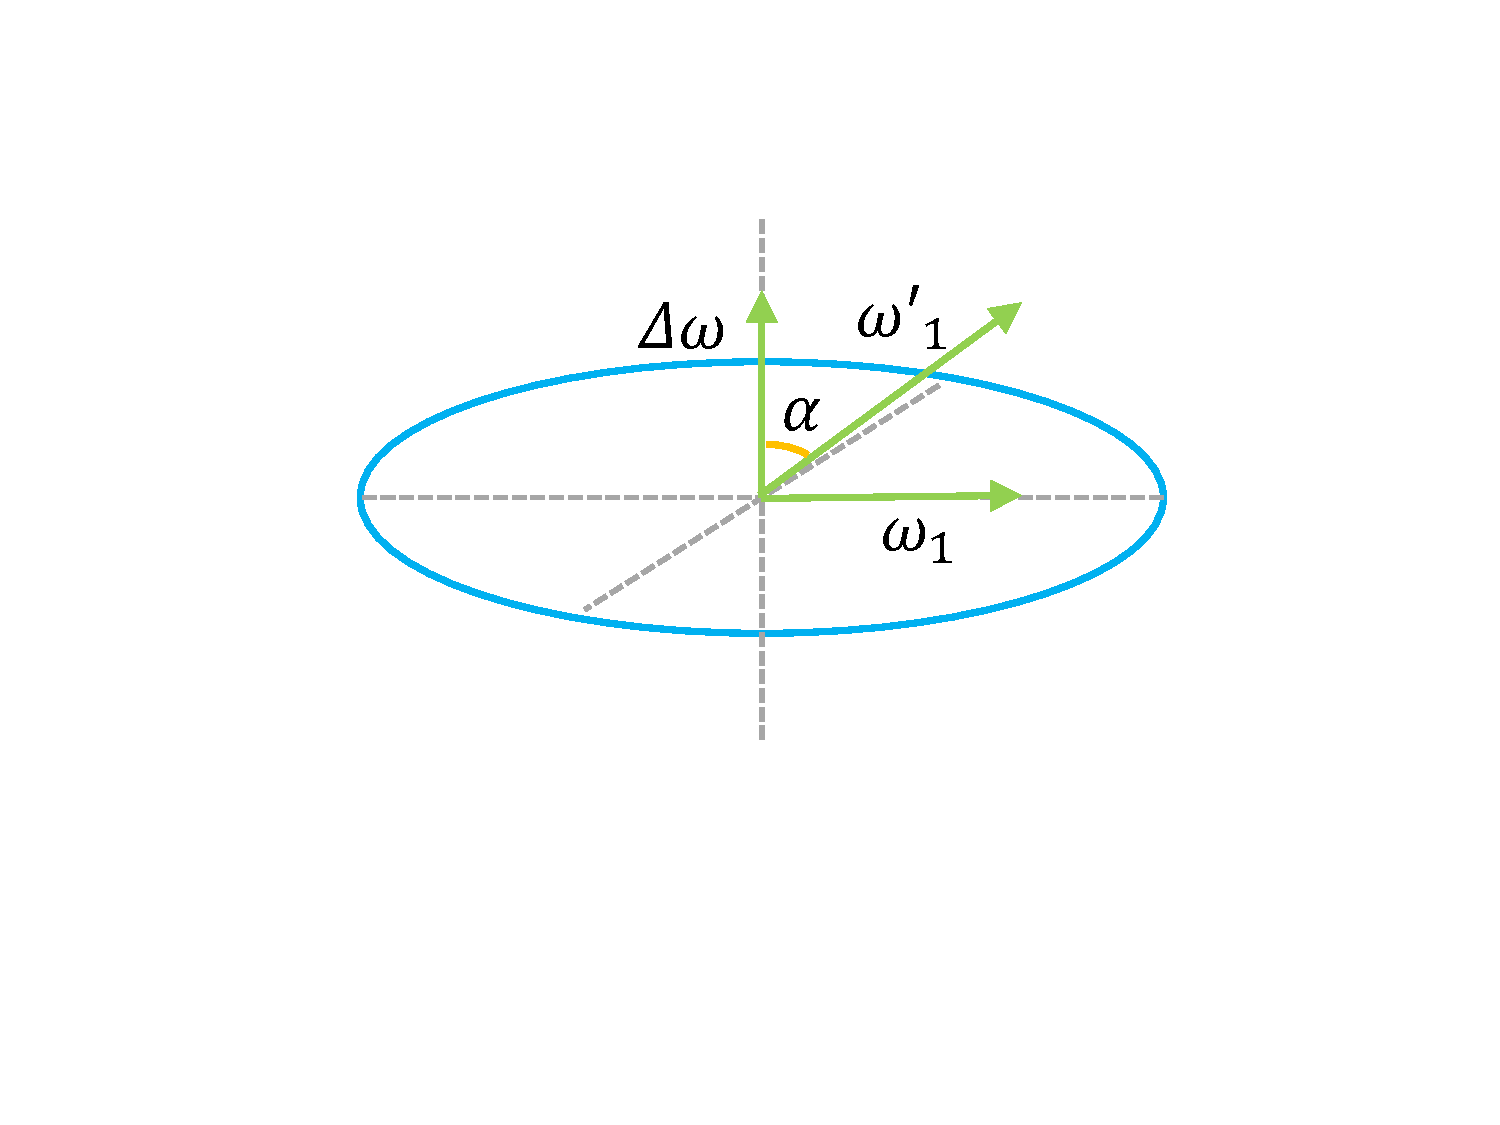
\includegraphics[width= 0.8\columnwidth]{figures/rotate.pdf}
              \caption{偏共振情况下,旋转坐标系中的旋转轴的变化示意图。
              }
              \label{rotate}
            \end{center}
\end{figure}

可以看出,当射频场远离自旋共振频率时,射频场对这个自旋几乎是没有影响的,因为当$|\Delta\omega\gg \omega_1|$时$\alpha$非常小。也就是说,当所有自旋都有分离的很好的Larmor频率的话,原则上我们可以选择性地旋转其中一个,同时对其他自旋没有任何操作。

和上面的旋转频率为$\omega_{rf}$不同,我们也可以选择频率为$\omega_0$的旋转坐标系,那么
\begin{equation}\label{aaa}
H^{rot} = -\hbar\omega_1(cos[(\omega_{rf}-\omega_0)t+\phi]I_x-sin[(\omega_{rf}-\omega_0)t+\phi]I_y).
\end{equation}
除非$\omega_{rf}=\omega_0$,这个变化并不能给出简洁的不含时射频哈密顿量。但对于不同的分离核自旋来说,该形式可以
针对不同的核自旋很好的给出旋转坐标系的形式
\begin{equation}\label{aaa}
\left\vert  \psi \right\rangle^{rot} =[\prod_i e^{-i\omega_0^itI_z^i}]\left\vert  \psi \right\rangle.
\end{equation}

如果是多旋转坐标系的话,射频场的哈密顿量可以类似给出
\begin{equation}\label{aaa}
H^{rot} = \sum_{i,r} -\hbar\omega_1^r(cos[(\omega_{rf}^r-\omega_0^i)t+\phi^r]I_x^i-sin[(\omega_{rf}^r-\omega_0^i)t+\phi^r]I_y^i),
\end{equation}
其中强度$\omega_1^r$和相位$\phi^r$依然是可控的。

在上式的射频场作用下,系统哈密顿量中的单量子项$I_z^i$将由于旋转坐标系的选取而被消掉,而余下的耦合项$J_{ij}I_z^iI_z^j$并不会演化,所以在多旋转坐标系中,
NMR体系的哈密顿量可以表示为
\begin{equation}\label{aaa}
H = H_{sys}+H_{control},
\end{equation}
其中内部哈密顿量为
\begin{equation}\label{aaa}
H_{sys} =  \hbar\sum_{i<j} 2\pi J_{ij}I_z^iI_z^j,
\end{equation}
而外部哈密顿量为
\begin{equation}\label{aaa}
H_{control} =  \sum_{i,r} -\hbar\omega_1^r(cos[(\omega_{rf}^r-\omega_0^i)t+\phi^r]I_x^i-sin[(\omega_{rf}^r-\omega_0^i)t+\phi^r]I_y^i).
\end{equation}

\subsection{弛豫和退相干机制}

利用核自旋作为qubit的一个优点就是NMR系统和周围的环境有很好的隔离,使得其退相干时间相比于动力学演化的时间可以很长。我们这里的讨论仅局限于
封闭系统的动力学演化,当然很多时候这个近似有一定的限制性。

NMR系统与环境的相互作用可以通过一个外加的哈密顿量$H_{env}$来描述。相比于$H_{sys}$ 或$H_{control}$来说它的作用比较小。量子信息的丢失,也就是退相干,正是源于该相互作用机制,一般又由
两个比例来描述:退极化过程(depolarizing)$T_1$ 以及退相位(dephasing)过程 $T_2$。

$T_1$是由自旋-晶格相互作用引起的,或者说在Larmor频率尺度上损失能量子的激发模式产生的,比如振动量子,顺磁离子,同溶剂间
存在离子交换的化学反应,或者有高阶磁矩的自旋等。在选择的比较好的分子及溶剂中,$T_1$的尺度大概为数十秒。NMR中的$T_1$机制类似于
其他物理系统中的非弹性散射,它会带来能量的损失。

$T_2$主要源于系统哈密顿量中没有被完全平均掉的自旋-自旋耦合。比如,在液体NMR分子中,一个分子内的自旋可能和
其他分子中的自旋有很弱的长程相互作用。其他的一些机制,例如化学位移的空间各向异性,顺磁离子等也对$T_2$的大小有一定的贡献。
尽管如此,在好的样品以及高磁场的NMR谱仪中,溶剂分子中的$T_2$可以轻易达到秒量级。$T_2$机制类似于其他物理系统中的弹性散射,系统并不会有任何的能量损失。

对于弛豫机制仅用两个参数来描述其实是对真实物理系统的过度简化,特别在耦合的自旋系统中,还有耦合弛豫机制在产生作用\cite{relax1,relax2}。尽管如此,独立的自旋
退相干模型依然非常有用,它可以很好的抓住主要效应,因为NMR量子计算中的脉冲序列时间基本都是短于$T_2$的。

\section{NMR中的脉冲技术}

前面已经提到,任何幺正操作都可以拆解为任意角度的单比特旋转门和两比特受控门,比如CNOT门的组合。
换句话说,如果要证明NMR量子计算是普适的,我们只需要能够有效实现任意角度的单比特旋转和CNOT门就可以了。在本节中,
我们将介绍如何利用NMR脉冲技术实现量子计算所需的逻辑操作。

\subsection{基本脉冲技术及单量子比特门的实现}

对于一个作用时间为$t_{pw}$的射频脉冲来说,如果它的强度为$\omega_1$且$\omega_{rf}=\omega_0$,那么
其作用的自旋感受到的幺正操作为
\begin{equation}\label{aaa}
U =exp[i\omega_1 (cos \phi I_x- sin \phi I_y)t_{pw}].
\end{equation}
该操作$U$描述的是Bloch球上在$\hat{x}-\hat{y}$平面内绕相位为$\phi$的轴转$\theta$角
\begin{equation}\label{aaa}
\theta =\omega_1 t_{pw}.
\end{equation}
那么,对一个精心设计过时间和相位的脉冲来说,它可以实现绕$\hat{x}$轴的$\pi /2$旋转,简记为$R_x(\pi/2)$或者$X$。如果把脉冲时间加倍,就可以实现$R_x(\pi)$,简记为$X^2$。通过改变射频脉冲
的相位,我们也可以执行$Y$和$Y^2$旋转。

原则上$\hat{x}$和$\hat{y}$方向的任意角度旋转可以实现所有的单比特任意角度旋转。比如要实现$Z$我们有两种基本的$X$和$Y$的组合脉冲可以利用
\begin{equation}\label{aaa}
Z = XY\overline{X} = Y\overline{X}\overline{Y}.
\end{equation}
要注意的一点是这里的操作是从右往左加的,并且对于以后出现的任何复合幺正操作都是如此。

我们可以通过施加一个足够长的软脉冲(soft pulse)选择性地激发一个自旋,同时不影响到分子中的其他自旋。这种软脉冲,或者叫形状脉冲(shape pulse)首先要把中心频率设置在要激发的自旋共振频率上,只影响一定频率范围内的核自旋(显然这个频率范围内不能覆盖其他的核自旋)。它从一个很低的强度$B_1$开始,逐渐加大到最大强度,再逐渐降低直至脉冲末尾。
一般来说,形状脉冲要分为几十甚至几百小片,通过改变每一小片的强度和相位,组合得到整个脉冲的强度和相位大小。对于脉冲宽度为$t_{pw}$的形状脉冲来说,傅里叶变换大概告诉我们它的频率范围为
$1/t_{pw}$。当然,这只是一个大致的结果,因为傅里叶变换是线性变化而射频场的变化是正弦型的,要得到精确的频率覆盖范围要用到其他的计算方法。

\begin{figure}[htbp]
            \begin{center}
              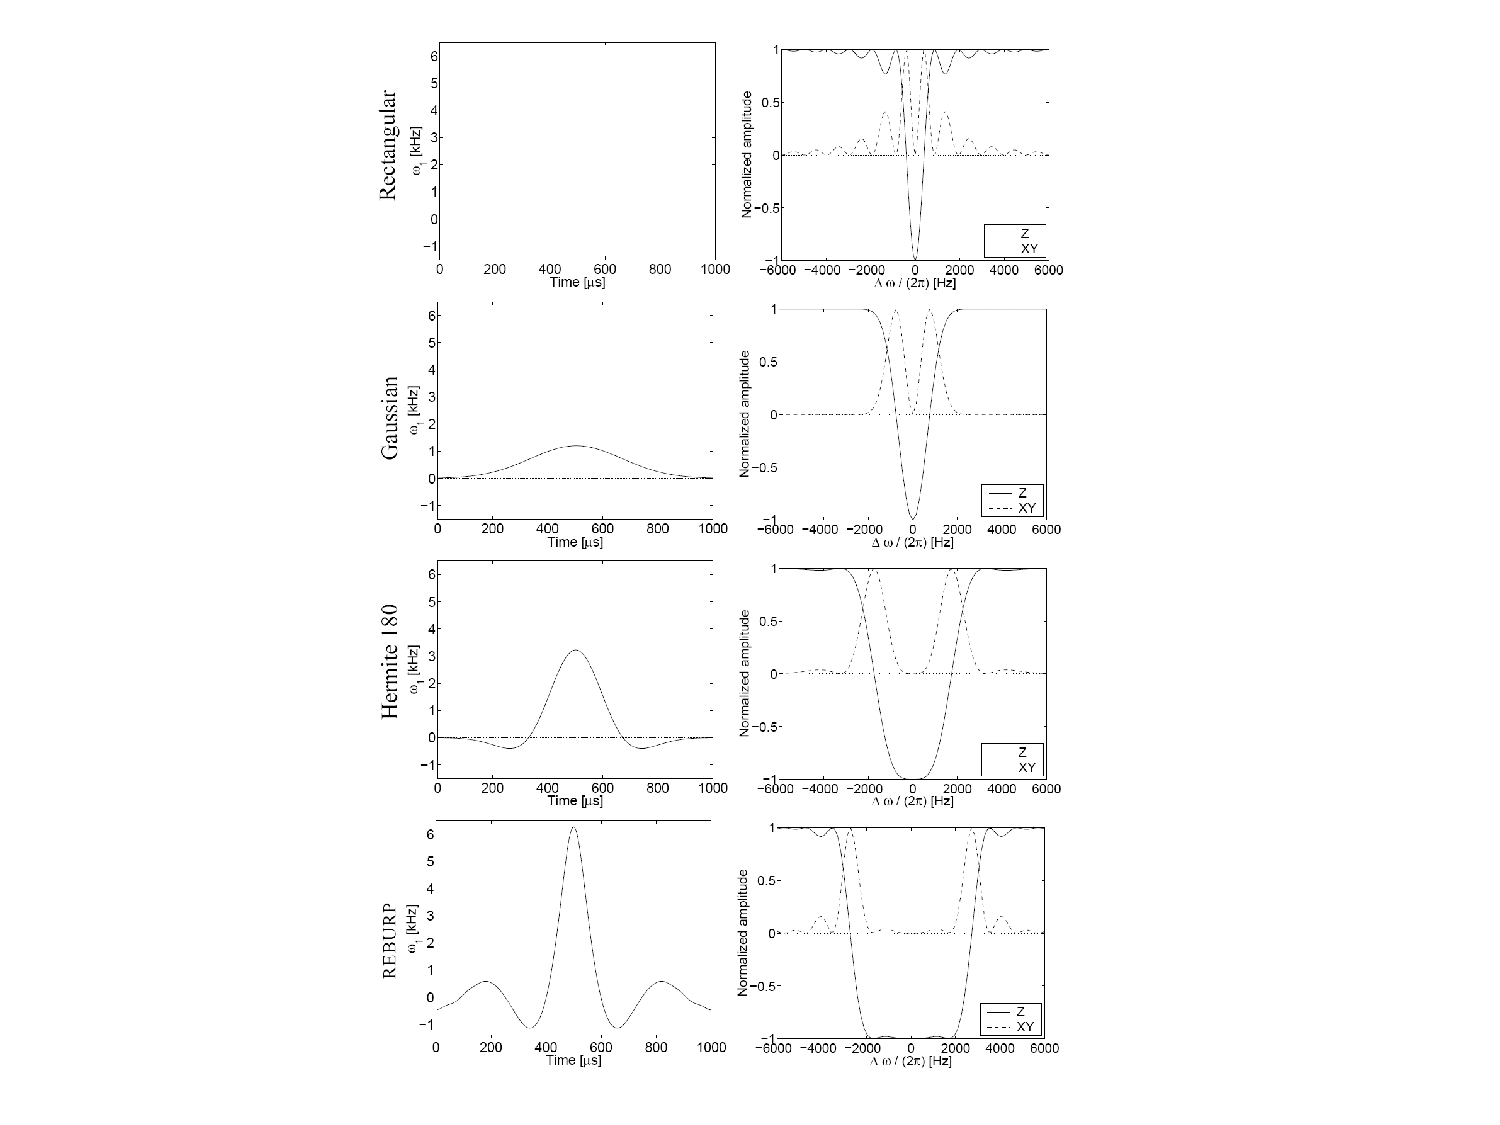
\includegraphics[width= 0.8\columnwidth]{figures/shape.pdf}
              \caption{常用的形状脉冲之间的脉冲宽度(左)与激发频率(右)比较。
              }
              \label{shape}
            \end{center}
\end{figure}

衡量形状脉冲的参数和指标很多,包括:

$\bullet$ 选择性:激发带宽与脉冲宽度的乘积,这个值越低说明选择的效果更好。这点很好理解,比如同样要选1000Hz的频率范围,如果形状脉冲A只用1$ms$就可以做到,而B需要10$ms$,显然A的选择性要比B好。

$\bullet$ 跃迁范围:除了需要的激发频率外,形状脉冲会影响到其他频率区域,这些区域就是跃迁范围。当然这个值越小越好。

$\bullet$ 脉冲强度:对于给定的脉宽,形状脉冲要求的峰值强度。这个值越低则该形状脉冲的要求越低。

 $\bullet$
 自回聚能力:能够回聚掉选择自旋与其他自旋间的$J$耦合的能力。这个值越大说明脉冲效果越好。

  $\bullet$
  鲁棒性:对于实验不完美性,比如射频场不均匀性等各种误差的灵敏度。这个值越大说明形状脉冲的抗噪声能力越强。

$\bullet$
普适性:形状脉冲是不是对任意的输入态或者只对特定输入态可以执行完美的旋转操作。

下表总结了常用的形状脉冲的特点\cite{shape1,shape2,shape3,shape4}。这些脉冲都是普适的,因为一般用于量子计算的态是任意态。明显可以看出,没有哪一个形状脉冲是所有
参数都是最优的,具体的脉冲选择要根据实验需求来定。比如,当化学位移的差别很大时,就没有必要要很小的
跃迁范围。

\begin{figure}[htbp]
            \begin{center}
              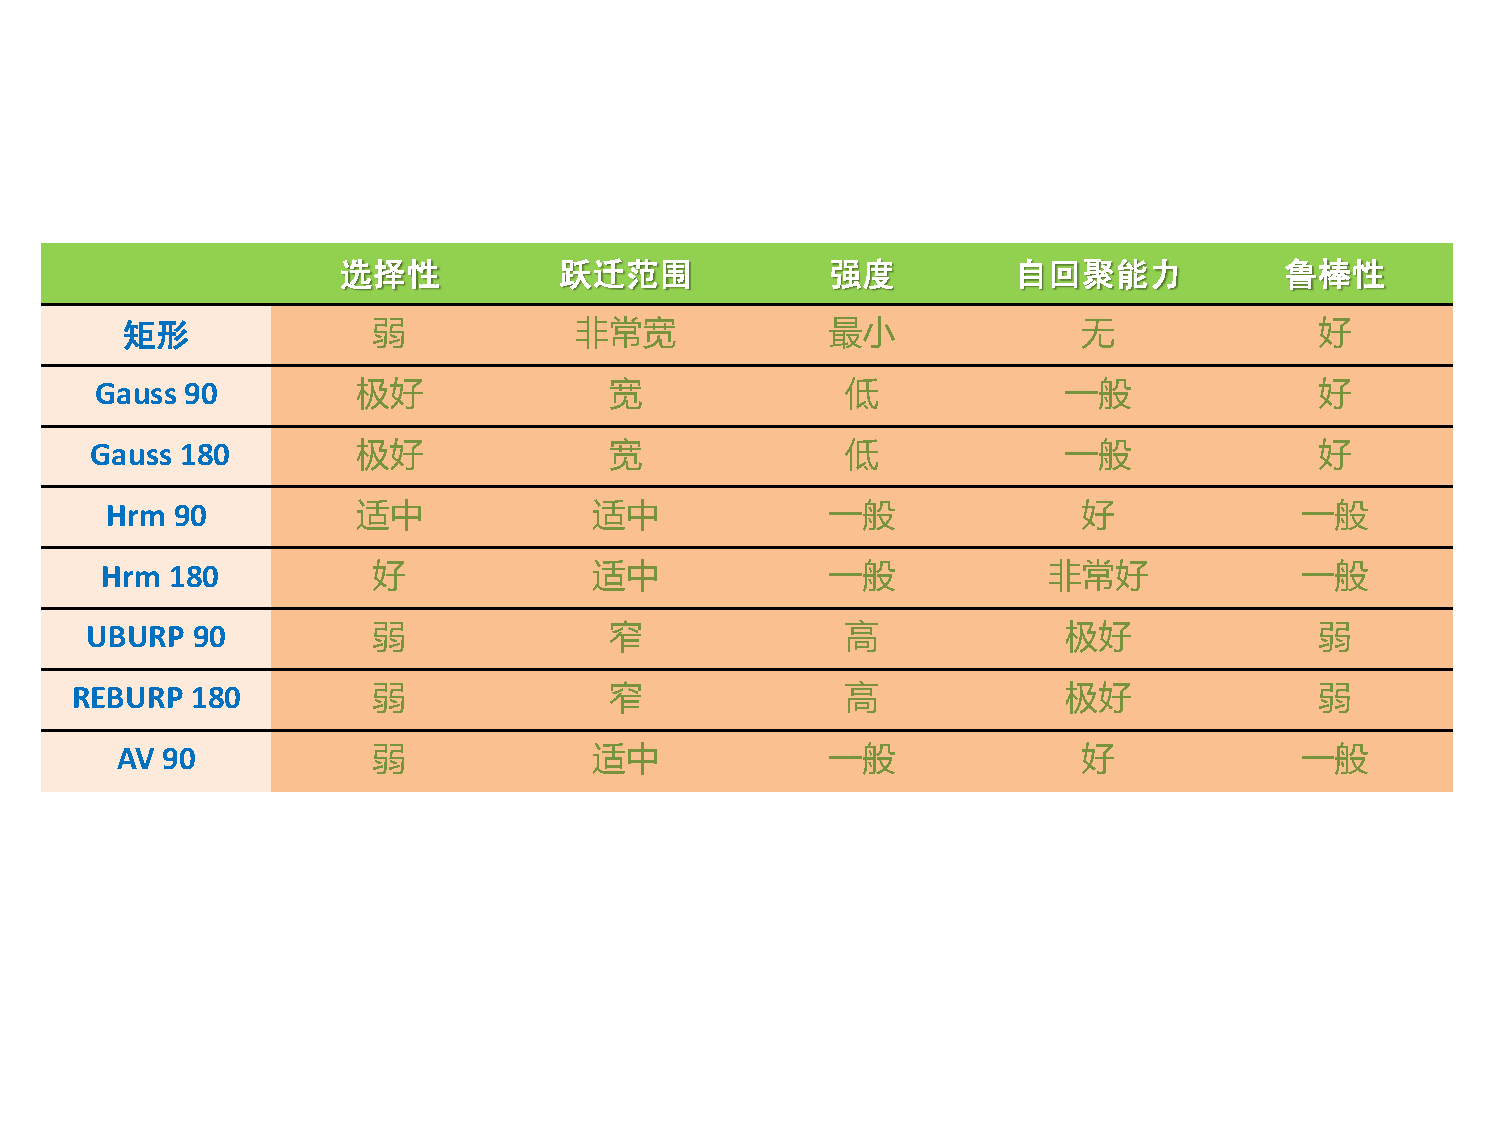
\includegraphics[width= 0.8\columnwidth]{figures/shapepara.pdf}
              \caption{各种形状脉冲之间的比较。
              }
              \label{shapepara}
            \end{center}
\end{figure}

对于异核分子来说,由于各个核之间的Larmor频率相差很大,所以激发不同核的脉冲几乎不需要选择性,所以其脉宽可以很短,比如10$\mu s$。这种脉冲的覆盖范围很大,一般可以覆盖所有同种原子核的频率。由于其强度相对于软脉冲非常大,所以叫做硬脉冲(hard pulse)。当然对于同核分子,比如$^{13}$C标记的Alanine中的三个$^{13}$C,要激发其中一个自旋的话我们不能用硬脉冲而只能选择软脉冲,或者后面将提到的更优秀的
GRAPE脉冲。

\subsection{脉冲重聚及两量子比特门的实现}

如果要实现CNOT门,最常见的方法是利用自旋间的耦合哈密顿量演化。从NMR的系统哈密顿量形式中,我们可以得到时间演化算子
\begin{equation}\label{aaa}
U_J(t) = e^{-i2\pi JI_z^1I_z^2t},
\end{equation}
或者其矩阵形式
\begin{equation}\label{aaa}
U_J(t) = \left(
           \begin{array}{cccc}
             e^{-i\pi J t/2} & 0 & 0 & 0 \\
             0 & e^{i\pi J t/2} & 0 & 0 \\
            0 & 0 & e^{i\pi J t/2} & 0 \\
             0 & 0 & 0 & e^{-i\pi J t/2} \\
           \end{array}
         \right).
\end{equation}
如果选择演化时间为$t = 1/2J$并在各个比特上加一个$\pi/2$的相移,我们将得到一个控制相位门(忽略掉全局相位)
\begin{equation}\label{aaa}
U_{CPHASE} = \sqrt{-i}\overline{Z_1}\overline{Z_2}U_J(1/2J)=\left(
           \begin{array}{cccc}
             1 & 0 & 0 & 0 \\
             0 & 1 & 0 & 0 \\
            0 & 0 & 1 & 0 \\
             0 & 0 & 0 & -1 \\
           \end{array}
         \right).
\end{equation}
CPHASE门的形式和CNOT门已经非常接近,控制比特上只差一个相位,而目标比特上只差简单的单比特旋转,
\begin{equation}\label{ucnot}
U_{CNOT} = iZ_1^2\overline{Y_2}U_{CPHASE}Y_2 = \sqrt{i}Z_1\overline{Z_2}X_2U_J(1/2J)Y_2=\left(
           \begin{array}{cccc}
             1 & 0 & 0 & 0 \\
             0 & 1 & 0 & 0 \\
            0 & 0 & 0 & 1 \\
             0 & 0 & 1 & 0 \\
           \end{array}
         \right).
\end{equation}
执行$U_{CNOT}$序列的核心是$X_2U_J(1/2J)Y_2$,其作用可以通过图\ref{nmrcnot}形象说明:假设两个自旋都处于$\pm \hat{z}$。首先自旋2绕$\hat{y}$旋转$\pi/2$,到达$\hat{x}$轴。然后整个系统在相互作用哈密顿量下自由演化$1/2J$的时间。由于自旋2的进动频率
依赖于自旋1所处的状态$\left\vert  1 \right\rangle$或者$\left\vert  0 \right\rangle$而会移动$\pm J/2$,自旋2在自由演化后所处的状态也会依赖于自旋1所处的状态而处于$+\hat{y}$或$-\hat{y}$轴。最后,自旋2绕$\hat{x}$旋转$\pi/2$。如果自旋1处于$\left\vert  0 \right\rangle$,自旋2将回到$+\hat{z}$;如果自旋1处于$\left\vert 1 \right\rangle$,自旋2将回到$-\hat{z}$。整体来看,当且仅当自旋1处于$\left\vert 1 \right\rangle$时,自旋2进行了翻转,而式\ref{ucnot}中的$\hat{z}$旋转则可以把所有的矩阵元调整到和$U_{CNOT}$完全一样。

\begin{figure}[htbp]
            \begin{center}
              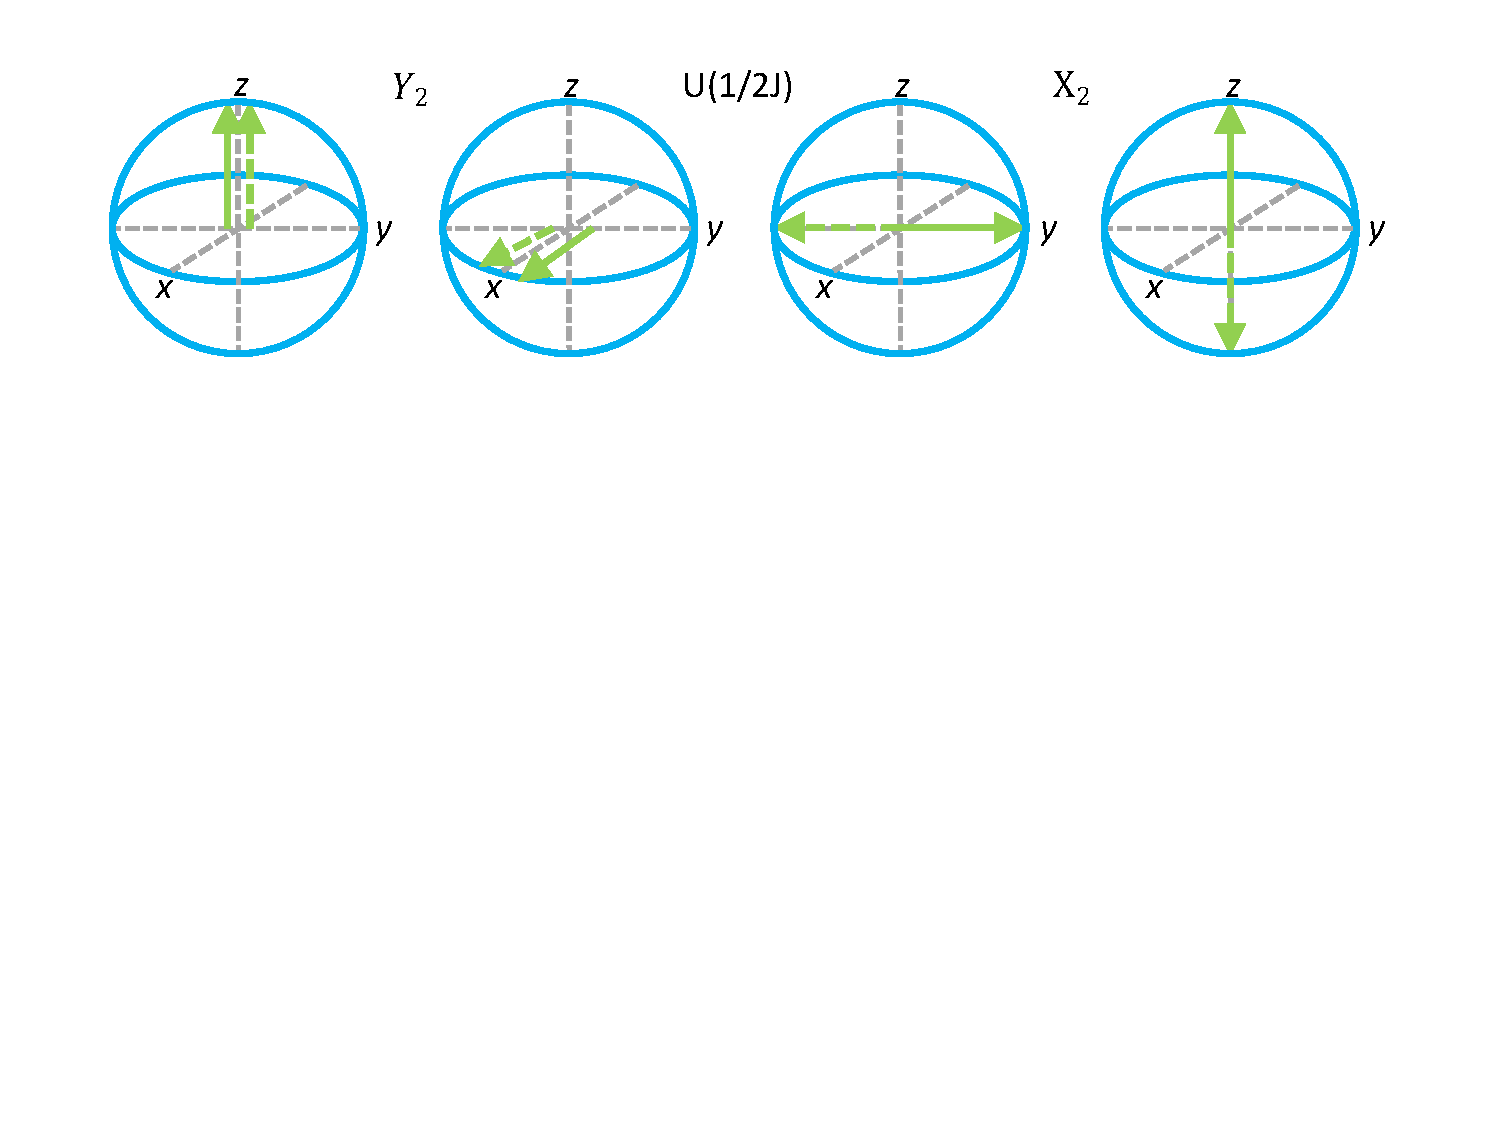
\includegraphics[width= 0.8\columnwidth]{figures/nmrcnot.pdf}
              \caption{CNOT门的Bloch球表示。目标比特2刚开始处于$\left\vert  0 \right\rangle$态,实线和虚线分别表示控制比特1处于$\left\vert  0 \right\rangle$和$\left\vert  1 \right\rangle$时qubit 2所处的状态。
              }
              \label{nmrcnot}
            \end{center}
\end{figure}

另外一种实现CNOT门的方法是利用线选脉冲。如果对处于频率$\omega_0^2+J/2$的峰施加一个选择性的$\pi$脉冲,它的作用是当且仅当控制比特1处于$\left\vert  1\right\rangle$时目标比特2将被翻转。当一个自旋和更多的自旋有耦合作用时,为了实现CNOT我们需要同时选择性地激发该自旋的一半的峰。目前实验上已经在五个qubit的系统上利用非常长的多频率激发脉冲 实现了CNOT门\cite{linecnot}。但当一个自旋的峰并没有分的很开时这种方法非常难以适用。

如果自旋间的相互作用哈密顿量不是$I_z^iI_z^j$的形式,还包括其他的横向分量,我们可以利用其他的脉冲序列
执行CPHASE和CNOT门,不过这些序列会很复杂\cite{linecnot2}。

如果两个自旋间并没有直接的相互作用,我们依然可以实现CNOT门,只要这两个自旋可以通过一系列的耦合连接起来。反过来,如果
一个自旋和很多的自旋间有相互作用,我们想执行它和另一个自旋间的CNOT的话则必须移除其他耦合的影响。一般来说,在NMR量子计算中常用的是已经在很多NMR实验中广泛运用的脉冲重聚技术。

在液体NMR中,耦合哈密顿量形式一般为$I_z^iI_z^j$,针对这种哈密顿量的重聚比较容易理解。如果耦合哈密顿量还包含横向分量的话,重聚过程就比较复杂了,需要运用平均哈密顿量的
理论来解释。

首先我们来看看如何在两qubit系统中消除$I_z^iI_z^j$形式的耦合。从数学形式来看,对于任意的演化时间$\tau$,总有
\begin{equation}\label{aaa}
X_1^2U_J(\tau)X_1^2 =U_J(-\tau) =X_2^2U_J(\tau)X_2^2,
\end{equation}
也就是
\begin{equation}\label{aaa}
X_1^2U_J(\tau)X_1^2U_J(\tau) =I=X_2^2U_J(\tau)X_2^2U_J(\tau).
\end{equation}
在上式中把所有的$X_i^2$替换为 $Y_i^2$,序列依然是类似的。如果有时用$X_i^2$,有时用 $Y_i^2$,我们得到的单位矩阵将有一些相位差别,但是如果同时在两个qubit上都加$\pi$脉冲的话,即
$X_1^2X_2^2U_J(\tau)X_1^2X_2^2U_J(\tau) $,耦合是不会被回聚的。

\begin{figure}[htbp]
            \begin{center}
              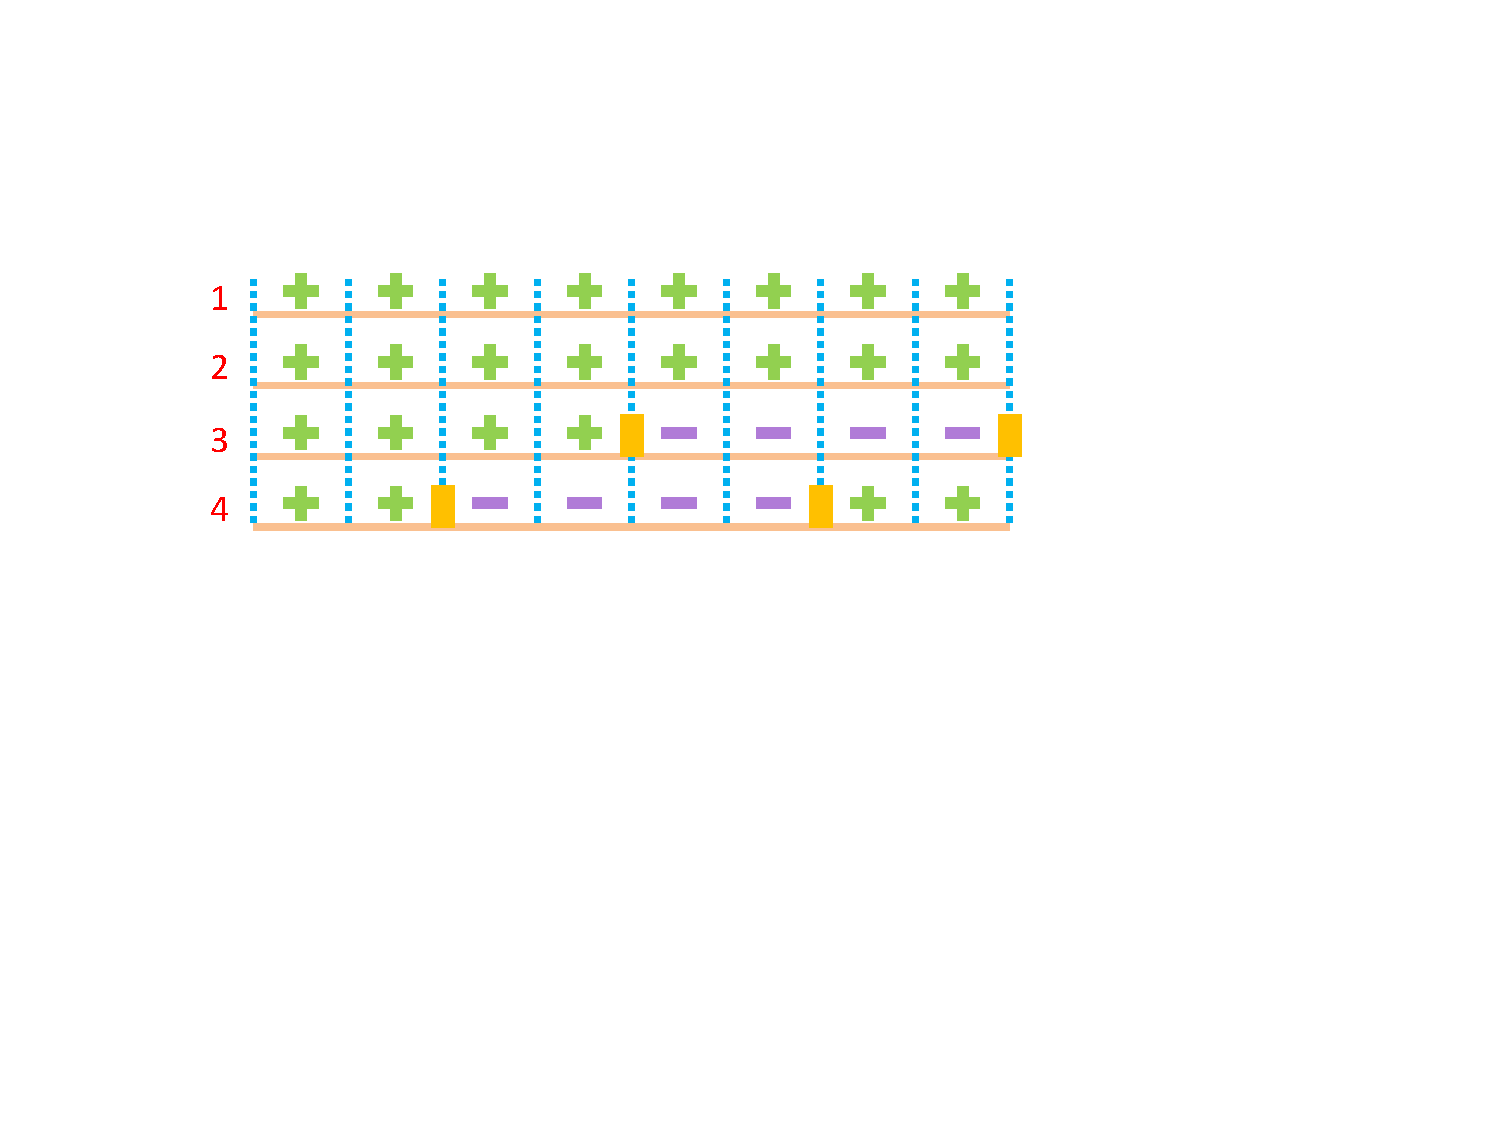
\includegraphics[width= 0.8\columnwidth]{figures/refocusing.pdf}
              \caption{四比特系统中只保留$J_{12}$形式的耦合的脉冲重聚序列。每一小段所代表的演化时间是相同的,黄色的矩形代表$\pi$脉冲,用来翻转当前自旋的状态。
              }
              \label{refocusing}
            \end{center}
\end{figure}

图\ref{refocusing}给出了多比特系统中的重聚技术。该序列有效地保留了$J_{12}$的效果,同时消除了其他耦合的影响。当一段耦合之内的自旋$i$和$j$处于相同的符号时,
可以认为耦合演化表现出来的效果是正方向的,而当两个自旋处于相反的符号时,耦合演化表现出来的效果是负方向的。只要一个耦合总体表现出来的正方向和负方向的时间是相同的,那么它的效果将
被回聚掉,没有任何影响。

在NMR量子计算中,设计重聚序列的系统化方法也已经发展起来。最常用的方案是基于Hadamard矩阵\cite{refo1,refo2}。
$n\times n$的Hadamard矩阵$H(n)$满足
\begin{equation}\label{aaa}
H(n)H(n)^T = nI.
\end{equation}
$H(n)$中所有行都是两两正交的,比如$H(12)$的例子如下图\ref{hadamard}

\begin{figure}[htbp]
            \begin{center}
              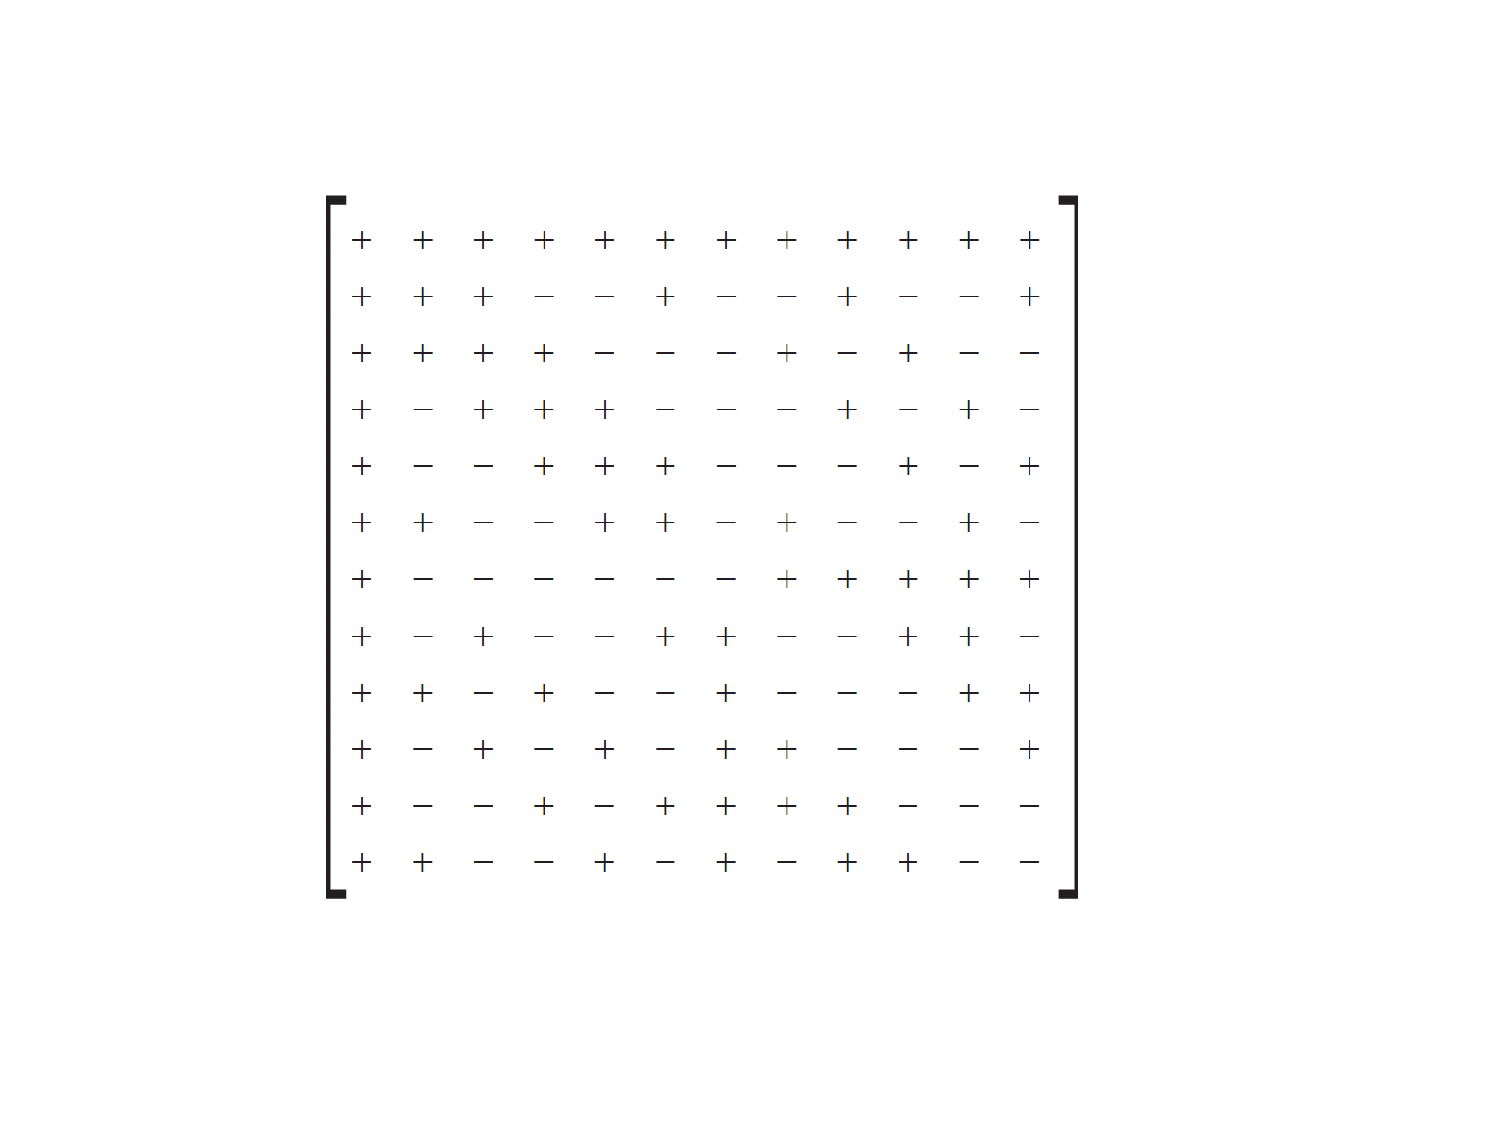
\includegraphics[width= 0.8\columnwidth]{figures/hadamard.pdf}
              \caption{重聚序列$H(12)$的形式。
              }
              \label{hadamard}
            \end{center}
\end{figure}

如果我们想保留任意一对耦合,同时回聚掉其他耦合的话,只需要简单的对$H(n)$中的那两个qubit用相同的行形式就可以了。

$H(n)$并不是对所有$n$都是存在的,但我们总可以找到一个$\overline{n}$,使得$H(\overline{n})$是已知的,且$\overline{n}\geq n$。因此对于$n$个自旋的系统我们需要$\overline{n}$个时间间隔来实现重聚,且$\pi$脉冲的个数不多于$n\overline{n}$个。

另外一种设计重聚序列的系统方法是Linden等人提出的\cite{refo3}。在四比特系统中,该序列形式如下
\begin{equation}\label{aaa}
\left(
  \begin{array}{cccccccc}
    + & + & + & + & +& +& + &+ \\
    + & + & + & + & - & - & - & - \\
    + & + & - & - & - & - & + & + \\
    + & - & - & + & + & - & - & + \\
  \end{array}
\right).
\end{equation}
每附加一个qubit,演化时间间隔的数量就翻倍,并且$\pi$脉冲在这个qubit上施加在第一,第三,第五个......时间间隔之后。同基于
Hadamard矩阵的方案相比,该方案不要求同时对多个qubit进行旋转,但该方案的时间间隔数目随着qubit的增加而指数增长。

%\subsection{梯度场技术}

%现代的NMR谱仪都配有在任意方向施加梯度磁场的线圈。假设梯度场的方向为$\hat{z}$方向,那么整个磁场的形式将是
%\begin{equation}\label{aaa}
%B(z) = B_0 + \gamma z B_1,
%\end{equation}
%其中$B_0$和$B_1$分别是静磁场和梯度场的强度。

\subsection{强调制脉冲及GRAPE脉冲技术}

在本章的第一节我们已经说过,对于同核系统来说,为了选择性地激发其中一个核自旋我们需要形状脉冲,但形状脉冲的缺点非常多。例如,它的强度比较低,也就意味着其作用时间很长,会带来
不可忽略的退相干效应,同时其作用时间内的内部哈密顿量演化也必须考虑。如果对一个NMR系统施加过多的形状脉冲,实验结果的误差将会是非常大的,量子计算的任务也不会有效的完成。

为了克服形状脉冲带来的低精度问题,2002年MIT的Cory小组提出了强调制脉冲(Strongly modulating pulses, SMP)\cite{smp1}理论,通过计算机的搜索和优化来强调制形状脉冲中的各个参数,从而精确实现所需的逻辑操作。由于SMP的脉冲能量一般很高,所以系统弛豫的影响将大大减小,同时优化过程中还能补偿一些系统误差的影响,例如射频场的不均匀性。
2005年,Glaser小组则利用梯度上升算法(gradient ascent pulse engineering, GRAPE)来设计形状脉冲,使得其效率和精度进一步提高。在本节中我们将简要介绍这两种在当前NMR量子计算领域极其重要的脉冲设计理论。

(a) \emph{强调制脉冲技术}

给出一个形状脉冲,我们可以轻松的计算出其演化算子,但反过来则非常困难。借助一些传统的分析技术,例如平均哈密顿量理论我们可以分析出合适的控制脉冲形式,但借助现代计算机及数学上的算法我们可以更有效且精确地给出
问题的解。从传统意义上说,强调制脉冲(Strongly modulating pulses, SMP)\cite{smp1,smp2,smp3}非常类似于形状脉冲。SMP中包含的脉冲数目并不算多,但是它们的强度,频率,脉宽以及相位都可以不同。强调制过程可以
理解为一种确定形状脉冲中各个参数的方法,其利用的多是数值模拟而非解析计算。 发展SMP技术的初衷是希望能够有效实现复杂的多自旋系统中的量子逻辑操作。在传统的方法中,例如利用自旋回波重聚技术来孤立哈密顿量中需要的项,然后构造逻辑网络图的方法在大的自旋体系中非常难以扩展。
上一小节中我们已经看到脉冲重聚随着比特数及相互作用数目增加时会变得非常复杂,而SMP的思路是通过不断改变和优化射频场的参数,并把所有的小片脉冲级联起来,使得整个脉冲的效果可以很好的实现需要的演化算子。
同时,在SMP中,很多系统误差,例如射频场的不均匀性等都可以考虑到优化过程中,使得最后搜索出来的SMP可以抗干扰。下面我们将给出SMP的设计方法。

首先,我们要确定如何衡量搜索得到的SMP所代表的幺正算子$U_{SMP}$和理论要求的幺正算子$U_{tar}$之间的相似程度,一般我们采用量子门保真度(quantum gate fidelity)的概念
\begin{equation}\label{aaa}
F = |\textbf{Tr}(U_{tar}^{\dagger}U_{SMP})/N|^2,
\end{equation}
其中$N=2^n$是Hilbert空间的维度。$F$越大,说明搜索到的SMP越好。关于保真度的具体讨论详见下一小节。

通过$F$,我们定义一个$Q$因子,
\begin{equation}\label{aaa}
Q = 1-\sqrt{F}.
\end{equation}
Q越小,也说明搜索到的SMP效果越好。在具体的程序中,我们就是用$Q$因子的大小作为衡量SMP的搜索结果的标准。

回忆本章刚开始时所讲过的,NMR系统的内部哈密顿量为
\begin{equation}\label{aaa}
H_{int} =-\hbar\sum_{i}\omega_0^i I_z^i+ \hbar\sum_{i<j} 2\pi J_{ij}I_z^iI_z^j.
\end{equation}
而外部哈密顿量也就是射频场的形式为
而外部哈密顿量为
\begin{equation}\label{aaa}
H_{ext} =  -\hbar\omega_1(cos[(\omega_{rf}-\omega_0^i)t+\phi]I_x^i-sin[(\omega_{rf}-\omega_0^i)t+\phi]I_y^i).
\end{equation}
从射频场的形式我们可以看出,射频场一共存在四个可变参数:能量$\omega_1$,频率$\omega_{rf}$,周期$t$和相位$\phi$。
那么演化算子
\begin{equation}\label{aaa}
U = e^{-i(H_{int}+H_{ext})t}.
\end{equation}
通过Nelder-Mead算法\cite{smp4},我们在整个空间内搜索这四个参数,使得$Q$因子尽可能的小。如果此时搜索得到的$U_{SMP}$和理论值$U_{tar}$之间非常接近,也就是$Q$很小,那么我们就保留这个结果并作为NMR实验上用的SMP。
但一般来说对于多自旋体系,单个的射频脉冲很难精确到获得所需操作,我们一般选择多个射频脉冲级联的方式,并且把每一小片脉冲中的
能量$\omega_1$定为常数,则有
\begin{equation}\label{aaa}
U_{net} = \prod_{m=1}^N U_m = \prod_{m=1}^N e^{-i(H_{int}+H_{ext}^m(\omega_1, \omega_{rf}^m, \phi^m, t^m))t^m}.
\end{equation}
序号$m$指的就是第$m$个方形脉冲小片。如果依然达不到所需结果,那么方形脉冲的数目还会继续增加。
%下面给出两个SMP的例子,分别是在3-qubit Alanine样品中的$R_x^3(\pi/2)$操作和4-qubit Crotonic中的 $R_x^{1,2}(\pi)$操作。

要注意的是,NMR实验并不会和理论计算的结果完全一样。在同一个样品中,处于不同位置的不同核自旋感受到的外磁场并不会完全一样,而且这些核自旋的化学位移也会
有轻微的差别。定义处于$\overrightarrow{r}$的自旋感受到的幺正操作为$U(\overrightarrow{r})$的话,整个NMR样品的密度矩阵演化过程大致可以写成一个非幺正的过程
\begin{equation}\label{aaa}
\rho(t) = \int U(\overrightarrow{r})\rho(0)U^{\dagger}(\overrightarrow{r})d\overrightarrow{r}),
\end{equation}
将化学位移和射频场的权重因子代入,则有
\begin{equation}\label{aaa}
\rho(t) = \int p(\omega,\Omega)U(\omega,\Omega)\rho(0)U^{\dagger}(\omega,\Omega)d\omega d\Omega).
\end{equation}
其中$\omega$是射频场的能量,而$\Omega$是化学位移。这是一个超算子的求和形式,其保迹条件为
\begin{equation}\label{aaa}
\int p(\omega,\Omega)d\omega d\Omega) =1.
\end{equation}

由于在实验中化学位移的变化对SMP的保真度影响并不大,我们着重考虑射频场不均匀性带来的影响。不均匀性的分布权重$p(\omega)$在实验上可以用
文献中的方法测出\cite{smp5},然后用新的含射频场分布权重因子的能量代替以前的射频能量
\begin{equation}\label{aaa}
\omega = \sum_{i = 1}^np(\omega_i)\omega_i,
\end{equation}
$n$为补偿不均匀性的取点个数,其值越大,修正就越好,但也会大大增加计算的复杂度。我们在实验上一般取3到5个点。

此时含射频场不均匀性的SMP的保真度形式为
\begin{equation}\label{aaa}
F = \sum_i|\textbf{Tr}(\sqrt{p(\omega_i)}U_{tar}^{\dagger}U_{\omega_i})/N|^2.
\end{equation}
至此我们就完成了SMP的射频场不均匀性的修正。

(b) \emph{GRAPE脉冲技术}

在多比特数时,SMP的方法并不是最优化的,而且SMP中每个脉冲小片都是方波,参数的跳变也会给具体的实验带来一定的误差。
德国的Glaser小组则从一个标准的优化控制思想出发,提出了GRAPE算法\cite{smp6}。

一个自旋体系的密度矩阵演化可以用Liouville Von-Neumann方程给出
\begin{equation}\label{aaa}
\dot{\rho}(t) = -i[(H_{int}+\sum_{k=1}^mu_k(t)H_{ext}),\rho(t)].
\end{equation}
$u_k(t)$是能够控制的射频场幅度因子。我们的目标是找到最优的$u_k(t)$,使得经过$T$时间演化后末态$\rho(T)$与理论要求的末态$C$之间尽可能的相似。
为了表征这个相似程度,我们采用两者的内积形式定义为表现因子
\begin{equation}\label{aaa}
\Phi_0 = <C|\rho(T)>.
\end{equation}

\begin{figure}[htbp]
            \begin{center}
              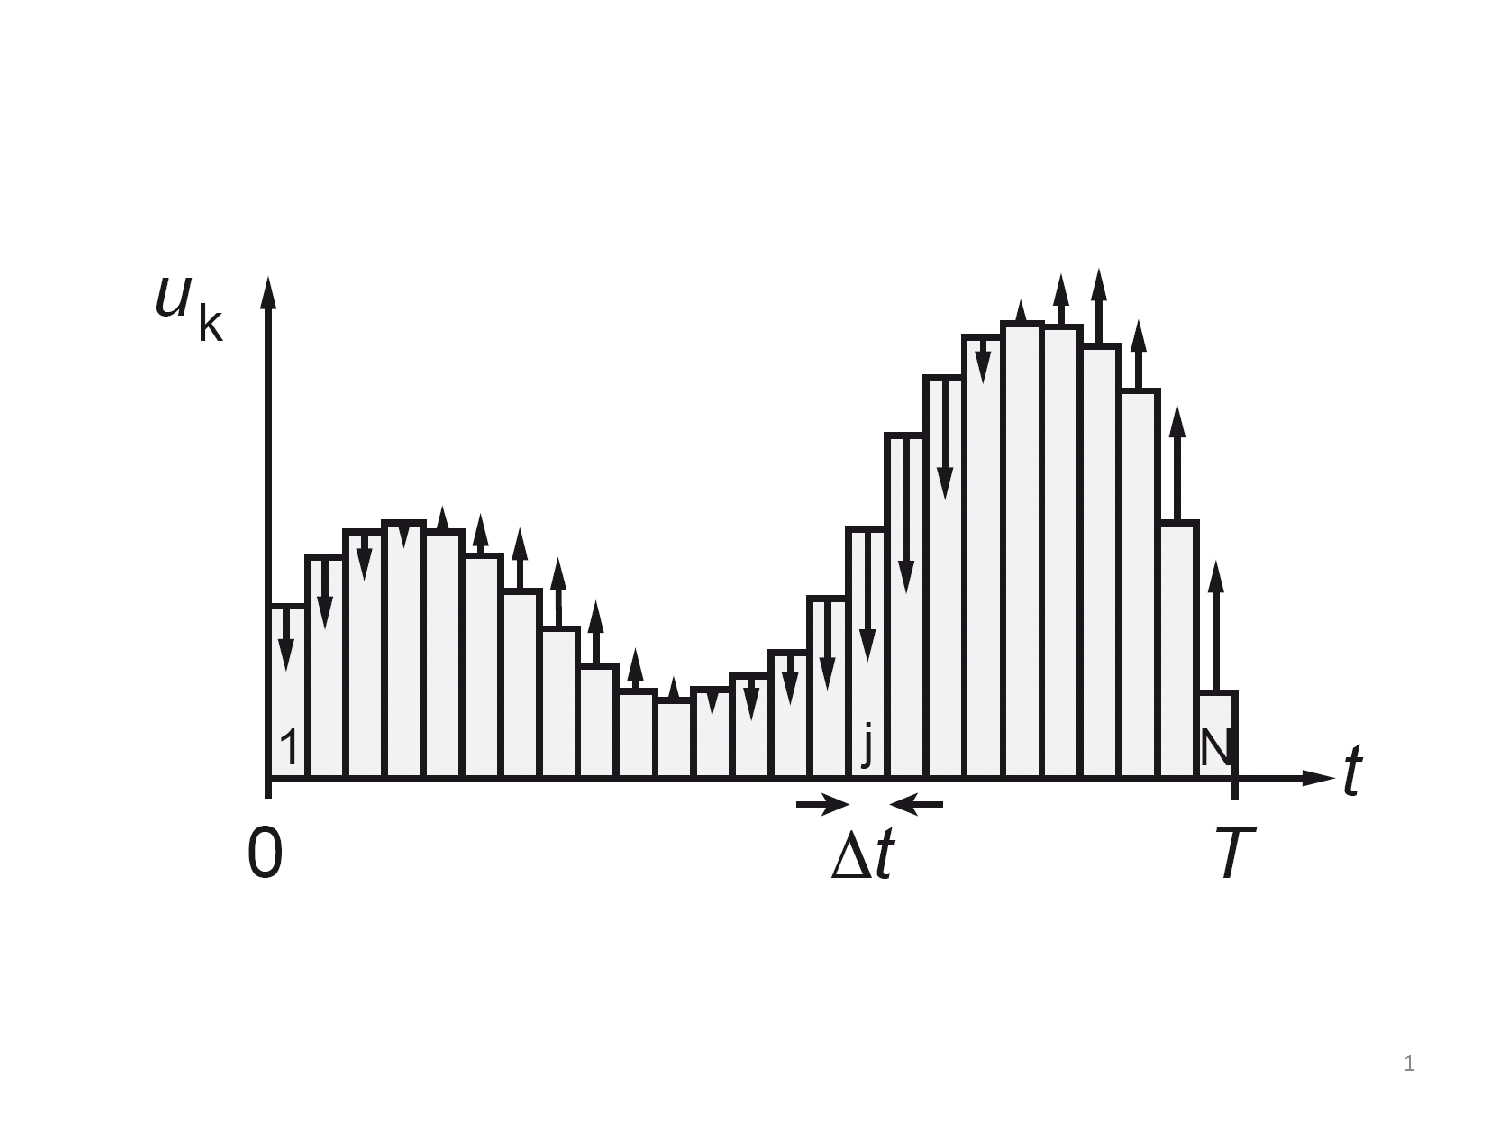
\includegraphics[width= 0.8\columnwidth]{figures/grape.pdf}
              \caption{在GRAPE算法中,每一小步的射频场幅度因子都是常数,而上下箭头表示的是幅度梯度。正是通过计算幅度梯度来改善整个GRAPE脉冲的效果(即$\Phi_0$的值)。
              }
              \label{grape}
            \end{center}
\end{figure}

整个演化时间被分为$N$步,每一步的时间间隔均为$\Delta t = T/N$,并保证每一步中,幅度因子$u_k$都是恒定的(见图\ref{grape})。那么第$j$步的演化算子为
\begin{equation}\label{aaa}
U_j = e^{-i\Delta t ((H_{int} + \sum_{k=1}^mu_k(j)H_{ext})},
\end{equation}
最后的末态密度矩阵为
\begin{equation}\label{aaa}
\rho(T) = U_N\cdots U_1 \rho_0 U_1^{\dagger}\cdots U_N.
\end{equation}
代入表现因子$\Phi_0$的表达式可得
\begin{equation}\label{aaa}
\Phi_0 = <C|U_N\cdots U_1 \rho_0 U_1^{\dagger}\cdots U_N>,
\end{equation}
并改写为
\begin{equation}\label{aaa}
\Phi_0 = <U_{j+1}^{\dagger}\cdots U_N^{\dagger} C U_N\cdots U_{j+1}|U_j\cdots U_1 \rho_0 U_1^{\dagger}\cdots U_j^{\dagger}>.
\end{equation}
后半部分$\rho_j$为$j\Delta t$时刻的密度矩阵,而前半部分$\lambda j$则可以看成是目标态$C$的反演。在某个$j\Delta t$ 时刻,我们通过测量$\Phi_0$的变化来改变$u_k(j)$,达到 $u_k(j)+\delta u_k(j) $。此时整个$U_j$的变化在一阶近似可以写成
\begin{equation}\label{aaa}
\delta U(j) = -i\Delta t \delta u_k(j) \overline{H_k} U(j).
\end{equation}
且
\begin{equation}\label{aaa}
\overline{H_k} \Delta t = \int_0^{\Delta t} U(j)(\tau)H_kU_j(-\tau)d\tau.
\end{equation}
当$\Delta t$趋近于0时,$\overline{H_k} \approx H_k$,即
\begin{equation}\label{aaa}
\frac{\Delta \Phi_0}{\Delta u_k(j)} = -<\lambda_j|i\Delta t[H_k,\rho_j]>.
\end{equation}
当我们采用的变化形式为
\begin{equation}\label{aaa}
u_k(j)\longrightarrow u_k(j) + \epsilon\frac{\Delta \Phi_0}{\Delta u_k(j)}
\end{equation}
时,表现因子$\Phi_0$的值可以被提升,也就是GRAPE的效果会变好。经过一次次的梯度上升,最终我们可以搜索得到精确的GRAPE脉冲。

如果在GRAPE算法中考虑射频场不均匀性的话,我们要采取的修正为
\begin{equation}\label{aaa}
\frac{\Delta \Phi_0}{\Delta u_k(j)} = \sum_i - 2p(\omega_i) Re(<P_j(\omega_i)|i\Delta t H_k X_j(\omega_i)>< X_j(\omega_i)|P_j(\omega_i)>).
\end{equation}

最后要提到的是,无论是计算SMP还是GRAPE脉冲,我们都需要对整个自旋系统进行完整的模拟。就像我们之前一直在提的,对于经典计算机来说
这个模拟过程所需要的资源是随着比特数的增加而指数增长的。其实,最好的设计SMP或GRAPE的方法就是利用一台量子计算机。当然,这有点类似“以子之矛攻子之盾”的含义,
但这确实是在量子计算发展中不可回避的问题,很多研究人员已经尽力在避免使用SMP或GRAPE脉冲了,或者使用精心挑选的
自旋系统来最大限度的规避这些问题。

\section{初态制备及测量读出}

\subsection{NMR中的赝纯态制备方法}

在NMR体系中,自旋初态一般为热平衡态
\begin{equation}\label{aaa}
\rho_{eq} = \frac{e^{-H_0/k_BT}}{\mathcal{Z}} = \frac{1}{\mathcal{Z}}\left(
                                                                       \begin{array}{cc}
                                                                         e^{-\hbar \omega_0/2k_BT} & 0 \\
                                                                         0 & e^{\hbar \omega_0/2k_BT} \\
                                                                       \end{array}
                                                                     \right).
\end{equation}
自旋所处的状态则由Boltzmann分布给出
\begin{equation}\label{aaa}
Pr[\left\vert 0 \right\rangle] = \frac{e^{-\hbar \omega_0/2k_BT}}{\mathcal{Z}} = \frac{e^{-\hbar \omega_0/2k_BT} }{e^{-\hbar \omega_0/2k_BT} +e^{\hbar \omega_0/2k_BT} }
\end{equation}
\begin{equation}\label{aaa}
Pr[\left\vert 1 \right\rangle] = \frac{e^{\hbar \omega_0/2k_BT}}{\mathcal{Z}} = \frac{e^{\hbar \omega_0/2k_BT} }{e^{-\hbar \omega_0/2k_BT} +e^{\hbar \omega_0/2k_BT} }.
\end{equation}
对于典型的NNMR磁场强度,比如10T,$\hbar \omega_0/k_BT\approx 10^{-5} \ll 1$,因此我们可以把指数项进行Taylor展开,得到
\begin{equation}\label{aaa}
\rho_{eq} \approx \frac{1}{2}\left(
                                                                       \begin{array}{cc}
                                                                         1+ \hbar \omega_0/2k_BT & 0 \\
                                                                         0 & 1 - \hbar \omega_0/2k_BT \\
                                                                       \end{array}
                                                                     \right).
\end{equation}
我们把$\varepsilon = \hbar \omega_0/k_BT$定义为自旋的极化度(polarization)。在热平衡态情况下,自旋的极化度几乎为0,自旋处于$\left\vert 0 \right\rangle$的概率$Pr[\left\vert 0 \right\rangle]$与处于$\left\vert 1 \right\rangle$的概率$Pr[\left\vert 1 \right\rangle]$几乎相等。

类似地,对于多自旋体系,热平衡态的形式为
\begin{equation}\label{aaa}
\rho_{eq} \approx \frac{1}{2^n}\left(
                                 \begin{array}{cccc}
                                   1+ \sum_k^n \frac{\hbar \omega_0^k}{2k_BT}  &  &  &  \\
                                    & 1- \frac{\hbar \omega_0^n}{2k_BT} + \sum_k^{n-1}\frac{\hbar \omega_0^k}{2k_BT} &  & \\
                                    &  & \ddots & \\
                                    &  &  & 1- \sum_k^n\frac{\hbar \omega_0^k}{2k_BT} \\
                                 \end{array}
                               \right).
\end{equation}
这里忽略了耦合能量是因为在10T左右的磁场下,$\hbar \omega_0$已经大约是$\hbar2\pi J_{ij}$的$10^6$倍了。

在热平衡态下,我们不可能知道自旋到底处于向上和向下的哪个状态,因为它们处于这些状态的概率几乎完全相等。
这种状态是不适合用作量子计算的初态的,我们需要的是一个单一的,能够确切知道的态(比如$\left\vert 00\ldots 0 \right \rangle$),所以我们必须寻找合适的方法实现NMR的初态制备。

最直观的纯化热平衡态的方法是通过冷却,把初态直接冷却到系统的基态上去。从极化度的表达形式可知,我们要求
热能$k_BT$ 远小于基态与第一激发态的能级差$\hbar \nu$。如果我们能够实现绝对零度,那这个要求自然就满足了。可惜的是这不是电子游戏,并不存在这种强大的冰系招数。对于Larmor频率在1GHz以下的NMR系统来说,这要求温度$T\ll0.05K$!很明显地液体NMR样品是做不到这一点的,因为它们肯定被冻住了。
目前能达到这一温度的NMR样品只有固体样品和液态的$^3$He\cite{pps1}。 以目前的技术手段来看,纯粹通过降温冷却实现NMR量子计算的初态制备是不现实的。

真正实现室温下NMR量子计算依赖于有效纯态(effective pure state)或者叫赝纯态(pseudo-pure state, PPS)的概念的提出。PPS的概念使得室温下进行NMR量子计算成为了可能,这些自旋的动力学行为看上去就和绝对零度时一模一样,至多有一个信号强度的差别。下面我们将解释NMR量子计算中非常重要的PPS的概念,并给出常用的
制备PPS的方法。

制备PPS的出发点首先依据的是NMR中非常重要的一个事实:NMR信号只和布居度之差有关,和布居度本身的大小并无任何关系。也就是说,一个单位矩阵在NMR中是不会产生任何信号的。同时,由于$UIU^{\dagger}=I$,单位阵也不会在
幺正操作下进行任何动力学演化。那么,在NMR中,我们只关心偏移密度矩阵(deviation density matrix)$\rho_{\Delta}$的概念,也就是在整个密度矩阵中减掉毫无用处的单位阵
\begin{equation}\label{aaa}
\rho_{\Delta} = \rho-I/2^n.
\end{equation}
这里我们已经假定$\rho$是归一化的,即$\textbf{Tr}(\rho) = 1$。

Gershenfeld和Chuang\cite{nmrpro2},以及Cory小组\cite{nmrpro1}分别独立发现下面的密度矩阵形式
\begin{equation}\label{aaa}
\rho_{eff} = \frac{1-\alpha}{2^n}I +\alpha \left\vert \psi \right \rangle \left\langle \psi \right \vert
\end{equation}
的动力学性质和它的第二项$\left\vert \psi \right \rangle \left\langle \psi \right \vert$相同,而$\left\vert \psi \right \rangle \left\langle \psi \right \vert$代表了一个纯态。因此我们就叫$\rho_{eff} $ 为有效纯态或赝纯态。

假设$\left\vert \psi \right \rangle = \left\vert 00\ldots 0 \right \rangle$的话,可以写出
 \begin{equation}\label{aaa}
\rho_{eff} = \frac{1-\alpha}{2^n}\left(
                                   \begin{array}{cccc}
                                     1 &  &  &  \\
                                      & 1 &  &  \\
                                      &  & \ddots &  \\
                                      &  &  & 1 \\
                                   \end{array}
                                 \right)
 +\alpha \left(
                                   \begin{array}{cccc}
                                     1 &  &  &  \\
                                      & 0 &  &  \\
                                      &  & \ddots &  \\
                                      &  &  & 0 \\
                                   \end{array}
                                 \right).
\end{equation}
可以看出在PPS的表达式中,除了一项之外,所有的对角元都是相等的。

那么如何从热平衡态$\rho_{eq}$出发得到PPS$\rho_{eff}$呢?明显地,由于$\rho_{eq}$和$\rho_{eff}$的本征值并不相同,
这个PPS制备过程一定是非幺正的。目前主要用到的PPS制备方法有四种:逻辑标记法(logical labeling)\cite{nmrpro2},空间平均法(spatial averaging)\cite{nmrpro1},时间平均法(temporal averaging)\cite{pps2}以及猫态制备法(cat-state preparation)\cite{pps2}。逻辑标记法需要辅助比特,所有的量子计算任务运行在一个初始为PPS的Hilbert子空间内;时间平均法则把PPS拆解为几部分,每次实验分别制备一个部分,最后把
所有的NMR结果加起来;空间平均法类似于时间平均,只是平均过程是发生在空间上;猫态制备法则综合了逻辑标记和空间平均两个概念。我们将分别介绍这些PPS制备方法。

(a) \emph{逻辑标记法}

逻辑标记法\cite{nmrpro2,pps4}的主要思想是通过施加脉冲序列,重新分配热平衡态的布居度,使得一个子空间内的自旋处于
PPS,所有的计算任务都在这个子空间内进行。NMR中最早用到子空间概念的实验是观测Berry相\cite{pps5}。

在3 qubit的同核自旋系统中,其热平衡态的表达式为
\begin{equation}\label{aaa}
\rho_{eq} = \frac{1}{2^3}\frac{\hbar \omega_0^n}{2k_BT}\left(
                                                         \begin{array}{cccccccc}
                                                           3 &  &  &  &  &  &  &  \\
                                                            & 1 &   &   &   &   &   &   \\
                                                             &   & 1 &   &   &   &   &   \\
                                                             &   &   & -1 &   &   &   &   \\
                                                             &   &   &   & 1 &   &   &   \\
                                                             &   &   &   &   & -1 &   &   \\
                                                             &   &   &   &   &   & -1 &   \\
                                                             &   &   &   &   &   &   & -3 \\
                                                         \end{array}
                                                       \right).
\end{equation}
以量子计算的语言来看,这8个布居度分别代表$\left\vert 000 \right \rangle$,$\left\vert 001 \right \rangle$ 到$\left\vert 111 \right \rangle$态。在热平衡态的表达式中,由$\left\vert 000 \right \rangle$,$\left\vert 011 \right \rangle$,$\left\vert 101 \right \rangle$,$\left\vert 110 \right \rangle$四个态张成的子空间就是一个PPS。

为了简化接下来的逻辑操作,我们可以通过qubit 1和qubit 2上的幺正操作重把布居度重新分配为
 \begin{equation}\label{aaa}
\rho_{eq} = \frac{1}{2^3}\frac{\hbar \omega_0^n}{2k_BT}\left(
                                                         \begin{array}{cccccccc}
                                                           3 &  &  &  &  &  &  &  \\
                                                            & 1 &   &   &   &   &   &   \\
                                                             &   & 1 &   &   &   &   &   \\
                                                             &   &   & 1 &   &   &   &   \\
                                                             &   &   &   & -1 &   &   &   \\
                                                             &   &   &   &   & -1 &   &   \\
                                                             &   &   &   &   &   & -1 &   \\
                                                             &   &   &   &   &   &   & -3 \\
                                                         \end{array}
                                                       \right).
\end{equation}
此时子空间$|{ \left\vert 000 \right \rangle, \left\vert 001 \right \rangle, \left\vert 010 \right \rangle, \left\vert 011 \right \rangle|}$ 就是一个PPS了。这个PPS依赖于qubit 1的状态,当其处于$\left\vert 0 \right \rangle$ 时,就是我们上面提到的PPS,一般我们叫其$\left\vert 0 \right \rangle_1$子空间。在制备了逻辑标记的PPS后,在剩下的脉冲序列中我们只需要重聚掉qubit 1的影响,那么整个计算过程就等价于在qubit 2和qubit 3上的量子计算任务了。

PPS子空间的维度受限于热平衡态中处于相同布居度的态的数量。在同核系统中,该数值为$C_n^{n/2} = n!/[(n/2)!]^2$(假定$n$为偶数),可用的PPS子空间包含的qubit数目则是$k = log_2(1+C_n^{n/2})$。当$n$很大时,$k/n$是趋近于1的,比如$n=40$时$k=37$。对于异核系统来说,分析会复杂一些,一般来说$k/n$
会更小,但随着总的qubit数目$n$的增加,可用作PPS子空间的$k$增加的也很可观。除此之外,为了重新分配布居度所要执行的逻辑操作的数目和
$n$是呈多项式关系的。

那么逻辑标记法的信号强度是多少呢?回忆前面提过的NMR信号强度是和布居度之差相关的。对于$n$为偶数的同核系统,可以认为在$\rho_{eq}$中的 $C_n^{n/2} $个相同的布居度都为0(当$n$为奇数且很大时,这个值也非常接近0),而最大的布居度为$n\hbar \omega_0/2^n2k_BT$。因此最大的信号强度$S$是以$n/2^n$的形式扩展的。而逻辑标记法中由于只有一个实验,噪声是与$n$无关的,
所以整个实验的信噪比为
\begin{equation}\label{aaa}
\frac{S}{N}\propto \frac{n}{2^n}.
\end{equation}

(b) \emph{时间平均法}

时间平均法的思想是把一系列的实验谱加起来,而每个实验谱都对应于不同的初态制备序列,产生不同的布居度改变,而相加后得到的态与PPS的性质完全相同。
由于量子力学的线性叠加性,各个独立实验得到的末态叠加和先把初态叠加后进行实验的效果是完全一样的。下面我们将给出三种进行时间平均的途径。

最传统的时间平均法是对$n$个自旋的系统进行$2^n-1$次实验,每次实验都对除了基态布居度之外所有的布居度进行不同的循环改变。例如,对一个2 qubit自旋系统,其热平衡态为
\begin{equation}\label{aaa}
\rho_1 = \rho_{eq} =\left(
                      \begin{array}{cccc}
                        a &   &   &   \\
                          & b &   &   \\
                          &   & c &   \\
                          &   &   & d \\
                      \end{array}
                    \right),
\end{equation}
这里用$a, b, c, d$是为了表明这种方法对任意的初态布居度分配都适用。如果我们对后面的三个布居度进行如下幺正变换
 \begin{equation}\label{aaa}
U_p = U_{cnot12}U_{cnot21},
\end{equation}
那么得到
\begin{equation}\label{aaa}
\rho_2 = U_p\rho_{eq}U_p^{\dagger} =\left(
                      \begin{array}{cccc}
                        a &   &   &   \\
                          & d &   &   \\
                          &   & b &   \\
                          &   &   & c \\
                      \end{array}
                    \right).
\end{equation}
如果我们循环地加这个幺正操作
\begin{equation}\label{aaa}
U_p^2 = U_{cnot21}U_{cnot12},
\end{equation}
将得到
\begin{equation}\label{aaa}
\rho_3 = U_p^2\rho_{eq}U_p^{\dagger2} =\left(
                      \begin{array}{cccc}
                        a &   &   &   \\
                          & c &   &   \\
                          &   & d &   \\
                          &   &   & b \\
                      \end{array}
                    \right).
\end{equation}
然后我们把$\rho_1,\rho_2,\rho_3$加起来,将得到
\begin{equation}\label{aaa}
\rho_{eff} = \left(
                      \begin{array}{cccc}
                        3a &   &   &   \\
                          & e &   &   \\
                          &   & e &   \\
                          &   &   & e \\
                      \end{array}
                    \right) = e\left(
                      \begin{array}{cccc}
                        1 &   &   &   \\
                          & 1 &   &   \\
                          &   & 1 &   \\
                          &   &   & 1 \\
                      \end{array}
                    \right)+(3a-e)\left(
                      \begin{array}{cccc}
                        1 &   &   &   \\
                          & 0 &   &   \\
                          &   & 0 &   \\
                          &   &   & 0 \\
                      \end{array}
                    \right),
\end{equation}
其中$e = b+c+d$。

在该方法中的信噪比是多少呢?任意一个实验中基态能级的布居度为$n/2^n$,而所有$2^n-1$个实验中基态能级的布居度只是简单的相加。另一方面,
噪声是随着实验数目的增多以平方根的形式增长的。那么,当实验数目为$l = 2^n-1$时,信噪比为
\begin{equation}\label{aaa}
\frac{S}{N}\propto \frac{n}{2^n}\frac{2^n-1}{\sqrt{2^n-1}} = \frac{n}{2^n}\sqrt{l} .
\end{equation}
这个大小其实和逻辑标记法中累加$l$次实验所得到的信噪比是相同的。

另外一种时间平均的过程不再是进行循环的布居度改变了。实际上,对任意一组线性无关的$2^n-1$个布居度分布$diag(\rho_i)$来说,我们总可以求解一系列的权重$\nu_i$,使得
\begin{equation}\label{aaa}
\rho_{eff} = \sum_{i=1}^l \nu_i\rho_i.
\end{equation}
这个方法的好处是每一个初态制备的序列会比循环改变的方法简单很多,而且,在近似情况下PPS可以通过少得多的实验来叠加得到(当然精确的解还是需要$2^n-1$个实验)。

这个方法的缺点主要是信噪比并不是最优化的。对于$l$次实验来说,其信噪比为
 \begin{equation}\label{aaa}
\frac{S}{N}\propto \frac{n}{2^n}\frac{\sum_{i=1}^l \nu_i}{\sqrt{\sum_{i=1}^l \nu_i^2}} \leq \frac{n}{2^n}\sqrt{l} .
\end{equation}
等号仅仅在所有的权重$\nu_i$为1时成立。

最后一种时间平均的过程是利用直积算子的形式。比如我们对5个同核自旋的热平衡态密度矩阵进行Pauli展开的话
 \begin{equation}\label{aaa}
\rho_{eq} = ZIIII+IZIII+IIZII+IIIZI+IIIIZ,
\end{equation}
注意这里的$Z$指的不是沿$\hat{z}$方向的旋转,而是核自旋算符。
PPS的形式为
 \begin{eqnarray}\label{aaa}
\rho_{eff} = ZIIII+\ldots+IIIIZ + ZZIII+\ldots+IIIZZ+ \nonumber \\
ZZZII+\ldots+IIZZZ+ZZZZI+\ldots+IZZZZ+ZZZZZ.
\end{eqnarray}
总共包含$2^5-1=31$项。利用简单的CNOT操作,热平衡态中的$n=5$项可以转化到不同的另外$n=5$项,基于基本的CNOT门的定义
 \begin{equation}\label{aaa}
CNOT_{12}: II\rightarrow II, IZ \rightarrow ZZ, ZI\rightarrow ZI, ZZ\rightarrow IZ.
\end{equation}
对于$n$个同核自旋系统,我们最少需要$\lceil (2^n-1)/n \rceil$个不同的实验来制备所有的$2^n-1$项。

在这种方案中,其信噪比是优化的,因为所有的权重因子都相等
 \begin{equation}\label{aaa}
\frac{S}{N}\propto \frac{n}{2^n}\frac{2^n-1/n}{\sqrt{2^n-1/n}} = \frac{n}{2^n}\sqrt{l}.
\end{equation}

(c) \emph{空间平均法}

空间平均法\cite{pps6}的思想是利用一个含梯度磁场的脉冲序列来平均掉除了基态能级外其他所有能级的布居度。
梯度场的作用是可以让样品中处于不同位置的自旋以不同的频率进动,使得它们的相位近乎平均掉。当然,这个过程并不是真正的
平均掉所有相位,是可以通过一个反向梯度场重聚的。以密度矩阵的语言来解释的话,梯度场的作用是使所有的非对角元都变成了0(除了零量子相干)。

最容易理解空间平均法的形式是直积算子形式。比如对于两个同核自旋的体系,这个过程可以表示为如下形式
\begin{eqnarray}\label{aaa}
&ZI + IZ \nonumber \\
\underrightarrow{R_x^2(\pi/3)} &ZI + \frac{1}{2}IZ -\frac{\sqrt{3}}{2}IY \nonumber \\
\underrightarrow{Gz} &ZI + \frac{1}{2}IZ  \nonumber \\
\underrightarrow{R_x^1(\pi/4)} & \frac{\sqrt{2}}{2}ZI + \frac{1}{2}IZ -\frac{\sqrt{2}}{2}YI \nonumber \\
\underrightarrow{d(1/2J)} & \frac{\sqrt{2}}{2}ZI + \frac{1}{2}IZ +\frac{\sqrt{2}}{2}XZ \nonumber \\
\underrightarrow{R_y^1(-\pi/4)} & \frac{1}{2}ZI -\frac{1}{2}XI+ \frac{1}{2}IZ + \frac{1}{2}XZ +\frac{1}{2}ZZ\nonumber \\
\underrightarrow{Gz} &\frac{1}{2}ZI + \frac{1}{2}IZ +\frac{1}{2}ZZ.
\end{eqnarray}

在上面的方案中,有一半的初始极化度被梯度场打掉了。每增加一个自旋,打掉的极化度就在增加一倍,因此其信噪比
为
 \begin{equation}\label{aaa}
\frac{S}{N}\propto \frac{n}{2^n}.
\end{equation}

空间平均法在网络图上是可扩展的,对于六个同核自旋系统,其PPS制备的网络图如下。
\begin{figure}[htbp]
            \begin{center}
              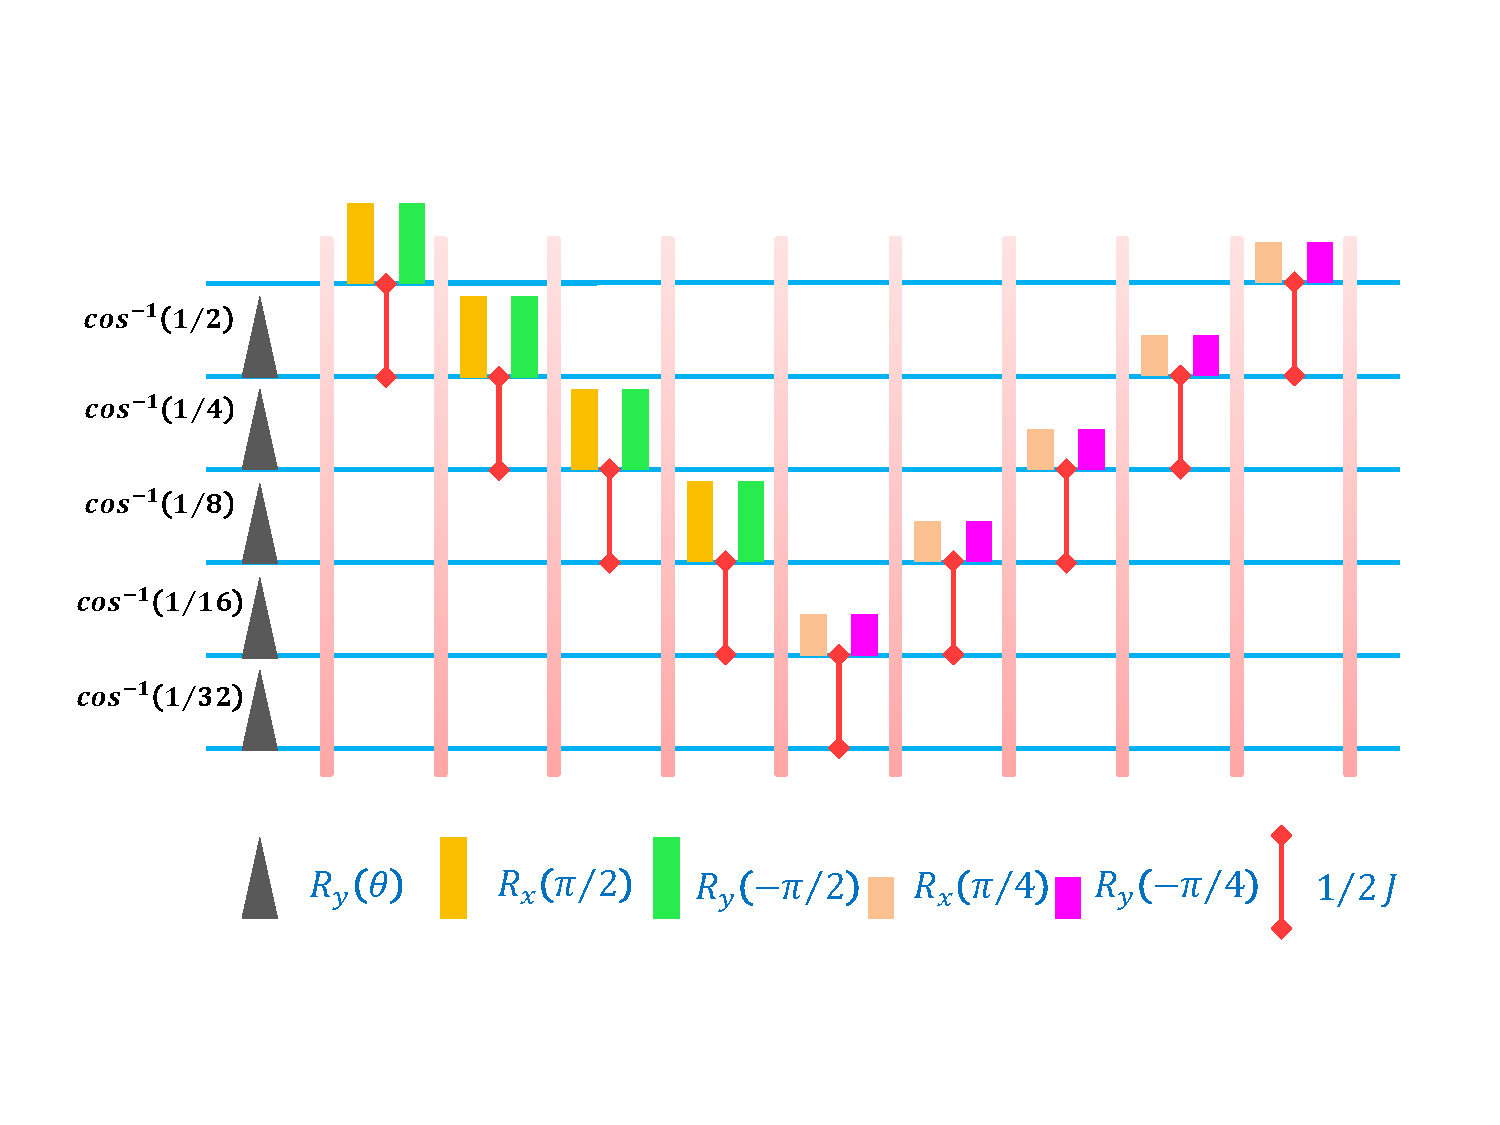
\includegraphics[width= 0.8\columnwidth]{figures/spatial.pdf}
              \caption{可扩展的6 qubit的PPS制备网络图。
              }
              \label{spatial}
            \end{center}
\end{figure}
理论上来说这个网络图是完全可以扩展到任意的$n$个qubit系统的。

(d) \emph{猫态制备法}

猫态制备法\cite{pps3}融合了逻辑标记与空间平均两种方法的思想。它即需要辅助位,也需要梯度场或者相循环来选择高阶相干。
所谓的猫态指的就是最大纠缠态,是以薛定谔的猫来命名的。在3 qubit情况,猫态就是一个GHZ态。从纯态出发,我们可以很轻易地制备猫态,比如四比特时其序列如图\ref{cat}。反过来的话,如果我们可以先制备猫态,自然也就可以得到赝纯态了。

\begin{figure}[htbp]
            \begin{center}
              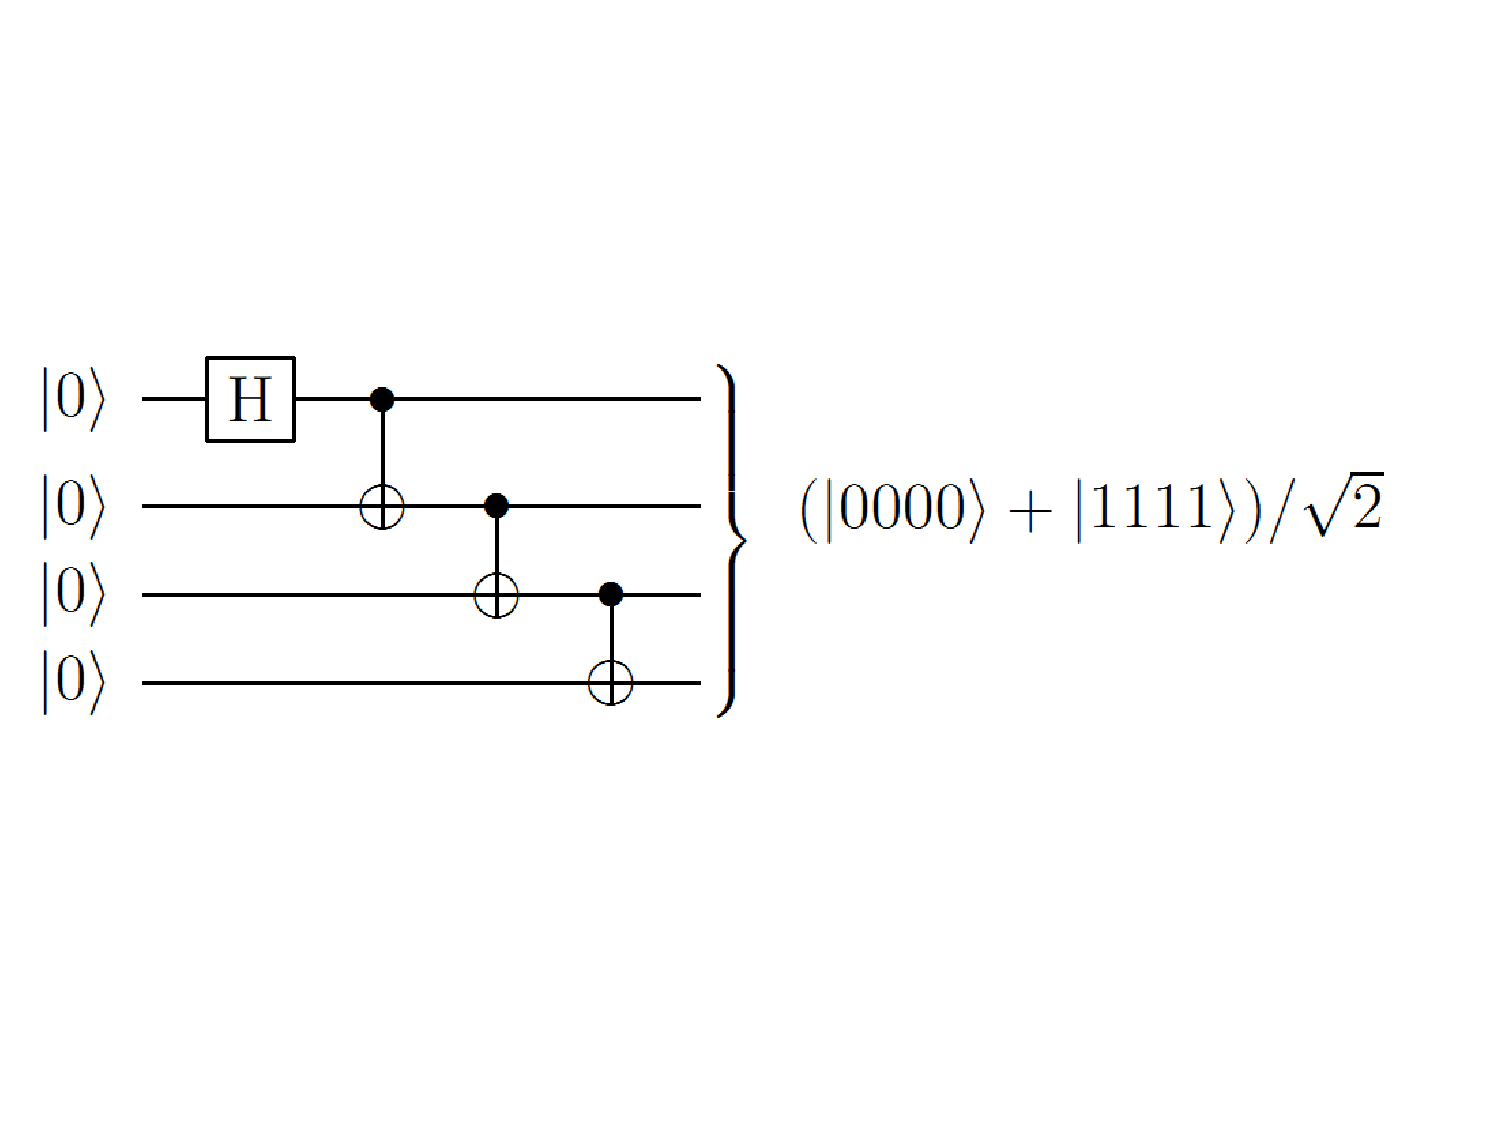
\includegraphics[width= 0.8\columnwidth]{figures/cat.pdf}
              \caption{4 qubit系统上制备猫态的逻辑网络图,仅需要Hadamard操作和CNOT操作。
              }
              \label{cat}
            \end{center}
\end{figure}

让我们考虑更加简单的3 qubit系统。制备猫态的网络图如图\ref{cat3}(a)所示。初态选择为$ZII$的话(这个态可以通过$\pi/2$旋转和梯度场很容易从热平衡态得到),经过该网络后,
系统的末态为$YYX$。该末态是含有三量子相干$ \left\vert 000 \right \rangle \left\langle 111 \right \vert+\left\vert 111 \right \rangle \left\langle 000 \right \vert$的,而这正是一个猫态的形式。在NMR中,不同阶的量子相干对于相位的敏感度是不同的,因此可以通过相循环
或者梯度场的方法把最高阶相干选择出来\cite{pps7}。然后通过图\ref{cat3}(b)所示的解码过程就可以得到逻辑标记的PPS:$X\left\vert 00 \right \rangle \left\langle 00 \right \vert$。

\begin{figure}[htbp]
            \begin{center}
              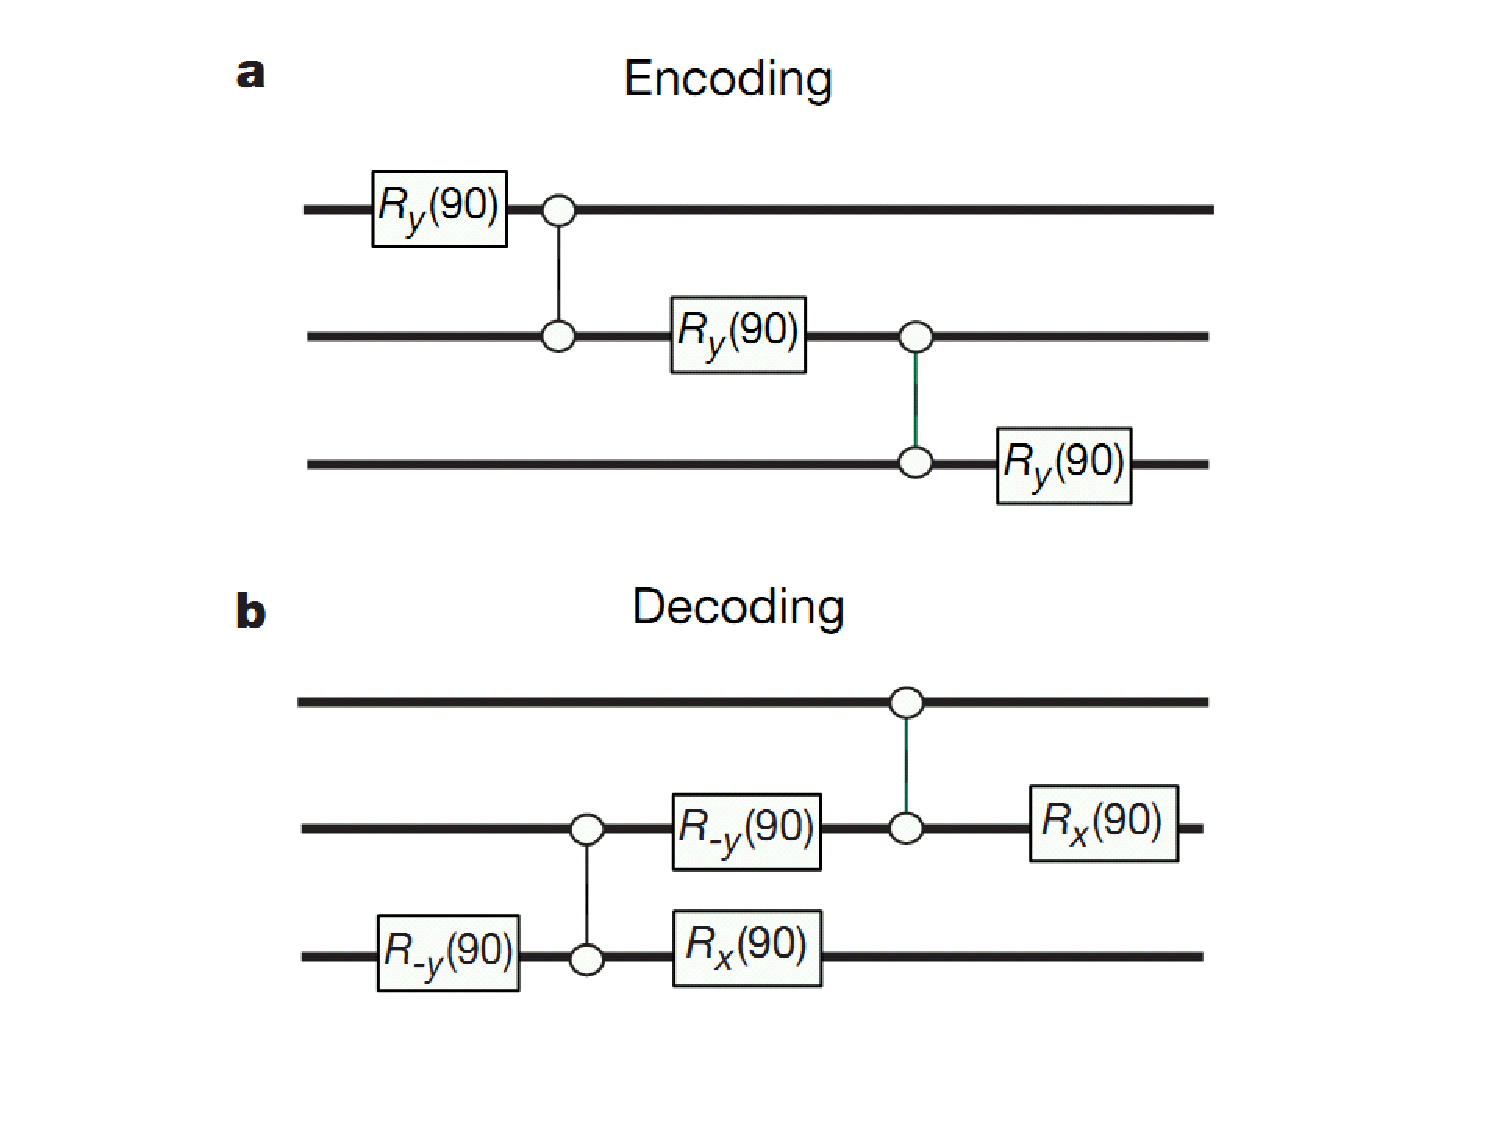
\includegraphics[width= 0.8\columnwidth]{figures/cat3.pdf}
              \caption{3 qubit系统上的猫态PPS制备法。(a) 从初态$ZII$出发,我们可以得到含有三量子相干$ \left\vert 000 \right \rangle \left\langle 111 \right \vert+\left\vert 111 \right \rangle \left\langle 000 \right \vert$的末态$YYX$。(b) 从三量子相干 $\left\vert 000 \right \rangle \left\langle 111 \right \vert+\left\vert 111 \right \rangle \left\langle 000 \right \vert$出发,可以得到逻辑标记后的纯态$X\left\vert 00 \right \rangle \left\langle 00 \right \vert$。取自[Nature 404, 368 (2000) \cite{pps3}]。
              }
              \label{cat3}
            \end{center}
\end{figure}

目前NMR量子计算领域最大qubit的实验就是利用猫态制备法制备了12 qubit的PPS\cite{12qubit},其网络图如图\ref{cat12}。

\begin{figure}[htbp]
            \begin{center}
              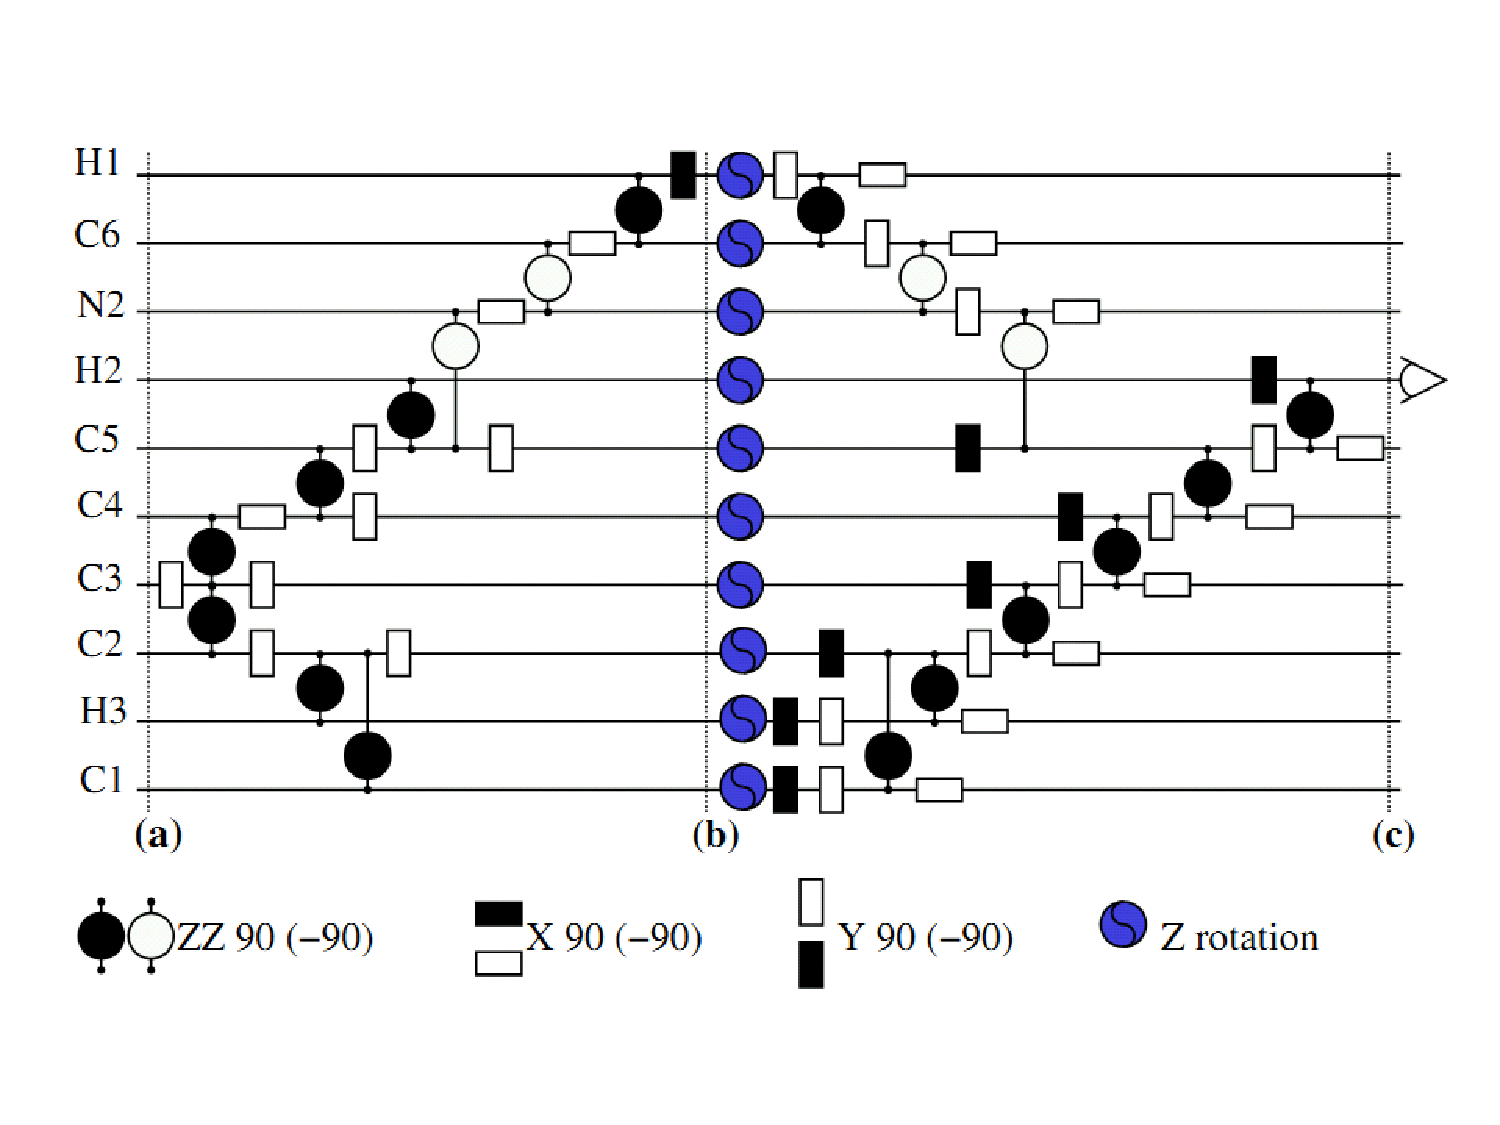
\includegraphics[width= 0.8\columnwidth]{figures/cat12.pdf}
              \caption{12 qubit系统上的猫态PPS制备网络图。取自[Phys. Rev. Lett. 96, 170501 (2006) \cite{12qubit}]。
              }
              \label{cat12}
            \end{center}
\end{figure}

在本节的最后,我们要注意两个问题。首先,所有的PPS制备方案要么对实验数量有指数的要求,要么信号强度会有指数的衰减。造成这种
衰减的原因很简单:这些方案只是简单地把基态能级的布居度选择了出来,而这个布居度的大小是正比于$n/2^n$的。这种指数衰减显然是和
量子计算的宗旨背道而驰的,但是在小量子系统的实验里不会有什么问题。

第二,也是很容易被人忽视的问题,就是我们只是在量子计算任务开始前进行了初态制备。但是很多量子计算方案要求在计算中也能进行
一些初始化过程,比如量子纠错。目前为止,没有合适的方案能做到这一点,当然有些方法原则上可以往这方面扩展。

\subsection{NMR中的读出手段}

单个核自旋的信号是非常难以探测的。目前只有离子阱及NV色心等少数体系中可以通过光学手段进行单自旋探测。在NMR中,我们观测的都是大量系综的统计平均
结果,典型的液体NMR样品大概要包含$10^{18}$个自旋用以观测。对所有的分子来说,它们感受到的操作是相同的,因此所有分子中自旋所处的末态也是相同的,可以进行简单的叠加。

NMR中的探测是通过配置在样品旁边的探测用射频线圈完成的。它可以探测自旋中磁矢量的横向分量,然后把这种时域信号通过傅里叶变化转换成
NMR谱。在NMR中,对于自旋状态的测量是弱测量(weak measurement),也就是探测线圈是一直工作的,但是与核自旋之间的耦合非常弱,因此对退相干几乎没有贡献。当然,由于与热库之间有相互作用以及
静磁场的不均匀性等依然会造成自旋状态的退相干,所以探测到的时域信号是随着时间衰减的,且一般为指数形式。这种由射频线圈采集到的
衰减时域信号叫做自由感应衰减(free induction decay, FID)。

如果FID的衰减形式是$e^{-t/T}$(一般来说$T = T_2^{*}$),那么FID的傅里叶变换将得到一个洛伦兹线型
\begin{equation}\label{aaa}
\propto \frac{1}{1+(\omega-\omega_0)^2}- \frac{i\omega}{1+(\omega-\omega_0)^2},
\end{equation}
且其半高宽为
\begin{equation}\label{aaa}
\Delta f = \frac{\Delta \omega}{2\pi} = \frac{1}{\pi T}.
\end{equation}
由于是弱测量,我们很难得到单个自旋状态的信息。但通过NMR样品中大量全同分子的叠加,我们可以得到想要的
关于平均自旋状态的很多信息。某种程度上来说,这些信息量比投影测量给出的信息量还要大。

测量得到的NMR信号的最大值$V_0$正比于

$\bullet$ 分子数量,与样品的体积$V$和浓度$n_c$有关。

$\bullet$ 分子中的全同原子核的数目$n_e$,比如CH$_3$Cl分子中的$^1$H的数目就为3。

$\bullet$ 热平衡态的自旋极化度$\epsilon_0$,和旋磁比$\gamma$,静磁场$B_0$,以及样品温度$1/T_s$成正比。

$\bullet$ $\omega_0$,与旋磁比$\gamma$和静磁场$B_0$成正比。

$\bullet$ 线圈的品质因子$Q$。

$\bullet$ 填充因子$\eta$,也就是样品在线圈中的占据程度。

$\bullet$ 因子$K$,反应了线圈的几何性质以及线圈与核自旋之间的耦合。

而测量的噪声主要是线圈的热噪声,和以下因素的平方根成正比

$\bullet$ 线圈的绝对温度$T_c$。

$\bullet$ 线路中的分流电阻$R = QL\omega_0$,其中$L$是电感。

$\bullet$ 音频过滤器的带宽$\Delta f$。

同时,NMR中的谱线强度不仅依赖于信号和噪声强度,还和信号在频率上的展宽有关。因此,NMR谱线的信噪比还正比于
$1/m$,$m$为谱线的数目,以及$T_2^{*}$(长的$T_2^{*}$可以给出更窄更高的谱线)。

总的来说,信噪比可以用如下形式表示
\begin{equation}\label{aaa}
\frac{S}{N} \propto \frac{n_cVn_e\gamma^2B_0^2Q\eta KT_2^{*}}{mT_s(T_cQL\gamma B_0\Delta f)^{1/2}} = \frac{n_cVn_e\gamma^{3/2}B_0^{3/2}Q^{1/2}\eta KT_2^{*}}{mT_s(T_cL\Delta f)^{1/2}} .
\end{equation}
关于信噪比的更深入的讨论,可以参见文献\cite{snr1}。

\subsection{NMR中的量子态重构}

对密度矩阵$\rho$的测量可以用来测试或者检验特定的量子态的制备过程。对于$n$个qubit张成的$2^n$维Hilbert空间内的单次测量来说,假定
要测量的态为$\left \vert m \right \rangle$,那么这个单次测量几乎给不出关于$\rho$的任何信息。可以从测量结果$m$推测出来的所有信息就只有
$Pr[\left \vert m \right \rangle]\neq 0$。

如果进行重复测量的话,每次都把系统制备到同样的状态并且在同样的基矢中测量,我们可以得到几率分布
\begin{equation}\label{aaa}
Pr[\left \vert m \right \rangle] =\left \langle m \right \vert \rho \left \vert m \right \rangle = Tr(\rho\left \vert m \right \rangle \left \langle m \right \vert) = Tr(\rho M),
\end{equation}
其中$M$是测量算子。如果我们对每个qubit都在$\{\left \vert 0 \right \rangle, \left \vert 1 \right \rangle\}$ 中重复测量的话,就可以得到密度矩阵中的所有对角元。

量子态重构(quantum state tomography)\cite{tomography1,tomography2,tomography3}是用能够确定出密度矩阵中所有元素的方法。通过在不同的测量基矢下重复测量相同的态,
以及求解线性方程组,我们就可以确定所有的元素。一般来说,我们会通过幺正变换把qubit旋转一个角度,然后在固定的基矢下测量。这和选取不同的基矢是等价的,因为
 \begin{equation}\label{aaa}
Tr[\rho (UMU^{\dagger})] = Tr[(U^{\dagger}\rho U)M].
\end{equation}
比如,单个qubit的密度矩阵可以展开成
 \begin{equation}\label{aaa}
\left(
  \begin{array}{cc}
    \rho_{00} & \rho_{01} \\
    \rho_{10} & \rho_{11} \\
  \end{array}
\right) = \rho_{00} \left \vert 0 \right \rangle \left \langle 0 \right \vert +\rho_{01} \left \vert 0 \right \rangle \left \langle 1 \right \vert+\rho_{10} \left \vert 1 \right \rangle \left \langle 0 \right \vert +\rho_{11} \left \vert 1 \right \rangle \left \langle 1 \right \vert.
\end{equation}
对其在$\{\left \vert 0 \right \rangle, \left \vert 1 \right \rangle\}$中测量的话我们首先可以得到$\rho_{00}$ 及$\rho_{11}=1-\rho_{00}$的值。然后,我们把基矢
绕$\hat{x}$轴转$\pi/2$,把$\rho$转化成$X\rho X^{\dagger}$,我们就可以得到$Im(\rho_{10}) = -Im(\rho_{01})$。类似地,绕$\hat{y}$轴转$\pi/2$ 的话我们可以得到$Re(\rho_{10}) = Re(\rho_{01})$。因此,三次测量就可以让我们重构整个密度矩阵$\rho$。

对于$n$个qubit的体系,我们也可以把密度矩阵展开为
\begin{equation}\label{aaa}
\rho = \sum_{i = 0}^{2^n-1}\sum_{j=0}^{2^n-1} \rho_{ij}\left \vert i \right \rangle \left \langle j \right \vert,
\end{equation}
并选择一组基矢变换,可以得到$\rho$中的所有$4^n-1$个自由度。

如果我们选择利用Pauli基组而不是计算基矢展开的话,找到基矢变换会更加容易。对单qubit的密度矩阵,它的Pauli展开可以写成
\begin{equation}\label{aaa}
\rho = c_0 \sigma_0+c_1 \sigma_1+c_2 \sigma_2+c_3 \sigma_3,
\end{equation}
其中$c_0=1$为归一化条件,且$\sigma_0 = I/2, \sigma_1 = \sigma_x/2,\sigma_2 = \sigma_y/2,\sigma_3 = \sigma_z/2$。在计算基矢中的测量给出$Pr[\left \vert 0 \right \rangle] = (c_0+c_3)/2$,且 $Pr[\left \vert 1 \right \rangle] = (c_0-c_3)/2$ ,我们就可以解出$c_3$。而由于
\begin{eqnarray}\label{aaa}
X\rho X^{\dagger} = c_0 \sigma_0+c_1 \sigma_1-c_3 \sigma_2+c_2 \sigma_3, \nonumber \\
Y\rho Y^{\dagger} = c_0 \sigma_0+c_3 \sigma_1+c_2 \sigma_2-c_1 \sigma_3,
\end{eqnarray}
我们就可以在施加$X$后得到$(c_0\pm c_2)/2$,而在施加$Y$后得到$(c_0\mp c_1)/2$。

对于$n$个qubit,Pauli展开可以写成
\begin{equation}\label{aaa}
\rho = \sum_{i =0}^3  \sum_{j =0}^3 \cdots \sum_{k =0}^3 c_{ij\cdots k} \sigma_i\otimes \sigma_j \otimes\cdots \otimes \sigma_k,
\end{equation}
其中$c_{00\cdots 0}=1$为归一化条件。在计算基矢中的测量算子由以下形式给出
\begin{equation}\label{aaa}
(\sigma_0 \pm \sigma_3) \otimes (\sigma_0 \pm \sigma_3)\otimes\cdots \otimes (\sigma_0 \pm \sigma_3),
\end{equation}
并给出相应的概率
\begin{equation}\label{aaa}
\sum_{i,j,\ldots,k\in \{0,3\}} \pm \frac{c_{ij\cdots k}}{2^n}.
\end{equation}
例如对于2 qubit体系,有
\begin{eqnarray}\label{aaa}
Pr[\left \vert 00 \right \rangle] = (c_{00}+c_{03}+c_{30}+c_{33})/4, \\
Pr[\left \vert 01 \right \rangle] = (c_{00}-c_{03}+c_{30}-c_{33})/4,\\
Pr[\left \vert 10 \right \rangle] = (c_{00}+c_{03}-c_{30}-c_{33})/4,\\
Pr[\left \vert 11 \right \rangle] = (c_{00}-c_{03}-c_{30}+c_{33})/4,
\end{eqnarray}
这样我们就可以通过求解线性方程组得到$c_{03},c_{30},c_{33}$。然后,要得到其他的$c_{ij\cdots k}$的话我们则需要进行旋转,比如
\begin{equation}\label{aaa}
X_1Y_2(\sigma_0 + \sigma_2)\otimes(\sigma_0 + \sigma_1)X_1^{\dagger}Y_2^{\dagger} = (\sigma_0 + \sigma_3)\otimes(\sigma_0 - \sigma_3).
\end{equation}

最后要说的是,测量基矢并非一定要选择计算基矢,在NMR实验中,单qubit测量算子可以写成$-i\sigma_1 - \sigma_2$。而对于耦合起来的两个自旋,测量算子为
\begin{eqnarray}\label{opernmr}
2(-i\sigma_1 - \sigma_2)\otimes (\sigma_0 \pm \sigma_3),\\
(\sigma_0 \pm \sigma_3) \otimes 2(-i\sigma_1 - \sigma_2).
\end{eqnarray}
由于NMR的实验结果是大量分子的系综平均,这些算子的期望值可以通过单次的NMR谱线直接读出。
式\ref{opernmr}中的四个算子就对应于两自旋系统的四条NMR谱线,而相位测量则允许我们同时读出每条谱线的实部和虚部项,从而区分$\sigma_1$和$\sigma_2$的贡献。

在测量出末态后,我们需要对实验上测到的结果$\left \vert \phi \right \rangle$和理论预期$\left \vert \psi \right \rangle$进行比较。对于这点我们引入量子态保真度(quantum state fidelity)的概念。对于两个纯态 的情况,保真度的定义为
\begin{equation}\label{aaa}
F(\left \vert \psi \right \rangle, \left \vert \phi \right \rangle) = |\left \langle \phi | \psi \right \rangle|,
\end{equation}
简单来说就是两个态交叠程度的绝对值的大小。

更一般的情况,末态使用密度矩阵来表示的,因为密度矩阵语言可以描述由于退相干导致的量子态的混合,即混态。
描述一个纯态$\left \vert \psi \right \rangle$和混态$\rho$的保真度形式为
\begin{equation}\label{erty}
F(\left \vert \psi \right \rangle, \rho) = \sqrt{\left \langle \psi \right \vert \rho   \left \vert \psi \right \rangle},
\end{equation}
当$\rho =\left \vert \phi \right \rangle\left \langle \phi \right \vert $时这个形式就退化到两个纯态的情况。

而对于两个混态$\rho$和$\sigma$来说,它们之间的保真度则定义为
\begin{equation}\label{aaa}
F(\sigma, \rho) = Tr \sqrt{\sqrt{\sigma}\rho\sqrt{\sigma}}.
\end{equation}
在这个表达式中其实$\rho$和$\sigma$是对称的,而其中一个为纯态时就退化到了式\ref{erty}的情况。

实验上另外一个常用的衡量保真度的参数是相关性(correlation),其形式为
\begin{equation}\label{correlation}
C = \frac{Tr(\sigma \rho)}{\sqrt{Tr(\sigma^2)Tr(\rho^2)}}.
\end{equation}
一般来说,相关性的值要比保真度高一些。

\section{强耦合液晶NMR体系量子计算}

前面的章节我们主要集中于讨论耦合形式为$I^i_zI^j_z$形式的哈密顿量模型,也就是弱耦合近似下的$J$耦合模型。
液体中由于分子的快速滚动,偶极耦合的效果都被平均掉了,而液晶及固体样品中偶极耦合的效应会显现,导致其处理手段和液体NMR有很大的不同。本节我们就将着重分析如何
利用强耦合NMR体系进行量子计算,主要集中在液晶NMR体系。

\subsection{强耦合体系的处理方法}

在液晶体系中,偶极耦合的大小约为$0$到$20kHz$,这个值远大于J耦合的$0$到$200Hz$的量级。因此对于自旋$1/2$的液晶体系,其哈密顿量形式为
\begin{equation}\label{aaa}
H_{sys}=\hbar\sum_{i} \omega_i I_z^i + \hbar\sum_{i<j} 2\pi J_{ij}I_z^iI_z^j + \sum_{i<j} \pi D_{ij}(2I_z^iI_z^j-I_x^iI_x^j-I_y^iI_y^j),
\end{equation}
$D_{IJ}$是核自旋$i$和$j$之间的偶极耦合常数。在偶极耦合项中,由于存在两个和其他项不对易横向分量$I_x^iI_x^j$和$I_y^iI_y^j$,
才使液晶NMR体系展现出很多和液体不一样的性质。

考虑简单的两体情况并忽略掉$J$耦合,则哈密顿量可以简化为(省略$\hbar$)
\begin{equation}\label{aaa}
H_{sys}=\omega_1 I_z^1+\omega_2 I_z^2 +  \pi D_{12}(2I_z^1I_z^2-I_x^1I_x^2-I_y^1I_y^2),
\end{equation}
写成矩阵形式的话
\begin{equation}\label{aaa}
H_{sys}=\left(
          \begin{array}{cccc}
            H_{11} &   &   &   \\
              & H_{22}   & H_{23}   &   \\
              &   H_{32} & H_{33}   &   \\
              &   &   & H_{44}   \\
          \end{array}
        \right),
\end{equation}
其中
\begin{eqnarray}\label{aaa}
H_{11}& =& +\frac{1}{2}\omega_1 +\frac{1}{2}\omega_2+\frac{1}{2}\pi D, \nonumber \\
H_{22}& =& +\frac{1}{2}\omega_1 -\frac{1}{2}\omega_2-\frac{1}{2}\pi D, \nonumber \\
H_{33}& =& -\frac{1}{2}\omega_1 +\frac{1}{2}\omega_2-\frac{1}{2}\pi D, \nonumber \\
H_{44}& =& -\frac{1}{2}\omega_1 -\frac{1}{2}\omega_2+\frac{1}{2}\pi D, \nonumber \\
H_{23}& =& H_{32}  =-\frac{1}{2}\pi D.
\end{eqnarray}

该形式的四个本征态分别为$\left \vert \alpha\alpha \right \rangle$,$cos\theta \left \vert \alpha\beta \right \rangle+sin\theta \left \vert \beta\alpha \right \rangle$,$cos\theta \left \vert \beta\alpha \right \rangle-sin\theta \left \vert \alpha\beta \right \rangle$,$\left \vert\beta\beta \right \rangle$。这里
\begin{equation}\label{aaa}
tan(2\theta) = \frac{-\pi D}{\omega_1-\omega_2}.
\end{equation}

很自然地可以看出,这四个本征态不再是四个计算基态。我们把这四个态标记为量子计算中的
$\left \vert 00 \right \rangle$,$\left \vert 01 \right \rangle$,$\left \vert 10 \right \rangle$,$\left \vert11 \right \rangle$态的话,这依然是一个两比特体系。这样标记的好处是NMR的谱线对应的是两个本征态之间的跃迁,
那么和液体NMR中采用核自旋作为qubit的标记一样,每条谱线只会与量子计算中的两个能级相关,因此更加直观。当然,在这种标记方式下,核选脉冲的意义
将变得不明显,而线选脉冲由于是对一个跃迁进行操作,因此将发挥更大的作用。更加方便的是用SMP或者GRAPE脉冲,它们的精度会更高。同时注意一点,当附加一个
能够使哈密顿量对角化的幺正操作后,其实这两种标记方式是等价的。

该哈密顿量的四个本征态所对应的本征值分别是
\begin{eqnarray}\label{aaa}
E_1  &=& -\frac{1}{2}\omega_1 -\frac{1}{2}\omega_2+\frac{1}{2}\pi D, \nonumber \\
E_2& =& +\frac{1}{2} \sqrt{(\omega_1 - \omega_2)^2+\pi^2D^2}-\frac{1}{2}\pi D, \nonumber \\
E_3& =& -\frac{1}{2}\sqrt{(\omega_1 - \omega_2)^2+\pi^2D^2}-\frac{1}{2}\pi D, \nonumber \\
E_4 & =& +\frac{1}{2}\omega_1 +\frac{1}{2}\omega_2+\frac{1}{2}\pi D,
\end{eqnarray}
通过本征值我们可以得到NMR谱线中各条谱峰的位置为
\begin{equation}\label{aaa}
 +\frac{1}{2}\omega_1 +\frac{1}{2}\omega_2\pm\frac{1}{2}\pi D \pm \frac{1}{2} \sqrt{(\omega_1 - \omega_2)^2+\pi^2D^2}.
\end{equation}
而这四条谱峰的高度将正比于$(cos\theta+sin\theta)^2$,$(cos\theta-sin\theta)^2$。当$\pi D\ll \omega_1 - \omega_2$,也就是$tan(2\theta)\approx 0 $时,我们发现四条谱峰依然等高,这就退化到了液体NMR中的弱耦合近似情况。

\subsection{液晶NMR量子计算的具体过程}


在了解到哈密顿量形式及本征值和本征态的不同后,下一点就是液晶NMR中哈密顿量的各个参数的确定。和液体情况不同,液晶样品的哈密顿量形式
中由于所有项并不是两两对易的,我们不可能
在简单地通过热平衡态的NMR谱线得到其数值大小了。比较原始的确定哈密顿量各个参数的办法是通过二维Z-COSY实验\cite{lq2}。我们采用的是拟合的办法,其步骤如下:

1. 把样品溶于液体溶剂Acetone中,测出$J$耦合的大小,并将其代入哈密顿量形式中作为已知参数。

2. 对哈密顿量中的化学位移及偶极耦合常数作初始猜测,然后计算该猜测的哈密顿量形式对应的NMR热平衡谱中各条谱线的位置。

3. 把计算出来的各条谱线同实验上各条谱线的位置进行平方差求和运算,以确定两者之间的误差大小。如果足够小(1Hz之内),则保留这组参数,否则对当前的哈密顿量参数进行
扰动,并重新计算谱线。

4. 在得到所有参数后,我们将计算NMR谱线的强度并与实验结果对比,作为除谱线位置外的另一组对比参数。我们发现只要谱线位置符合的话,谱线强度也符合的很好。

目前,我们已经在2,3,4 qubit的液晶体系上实现了哈密顿量的解谱,并保证满足液晶中的序参量与几何性质要求\cite{lq1}。同时,这些样品上也都完成了PPS制备,以及执行了相应的量子计算任务,并得到了很好的实验结果。这些都说明
我们的解谱确定哈密顿量参数的过程是正确的。

当前实验室内常用的液晶样品包括:2 qubit的1-bromo-2,3,5-dichloro-benzene,3 qubit的3-bromo-1,2-dichloro-benzene,以及4 qubit的1-bromo-2-dichloro-benzene。所有溶剂均为ZLI1132液晶溶剂。这些样品其实是把苯环上的六个$^1$H用没信号的$Br$或者$Cl$代替,
而剩下的$^1$H由于化学结构上不对称就可以作为两能级的qubit使用,它们的结构图如图\ref{lqsample}所示。

\begin{figure}[htbp]
            \begin{center}
              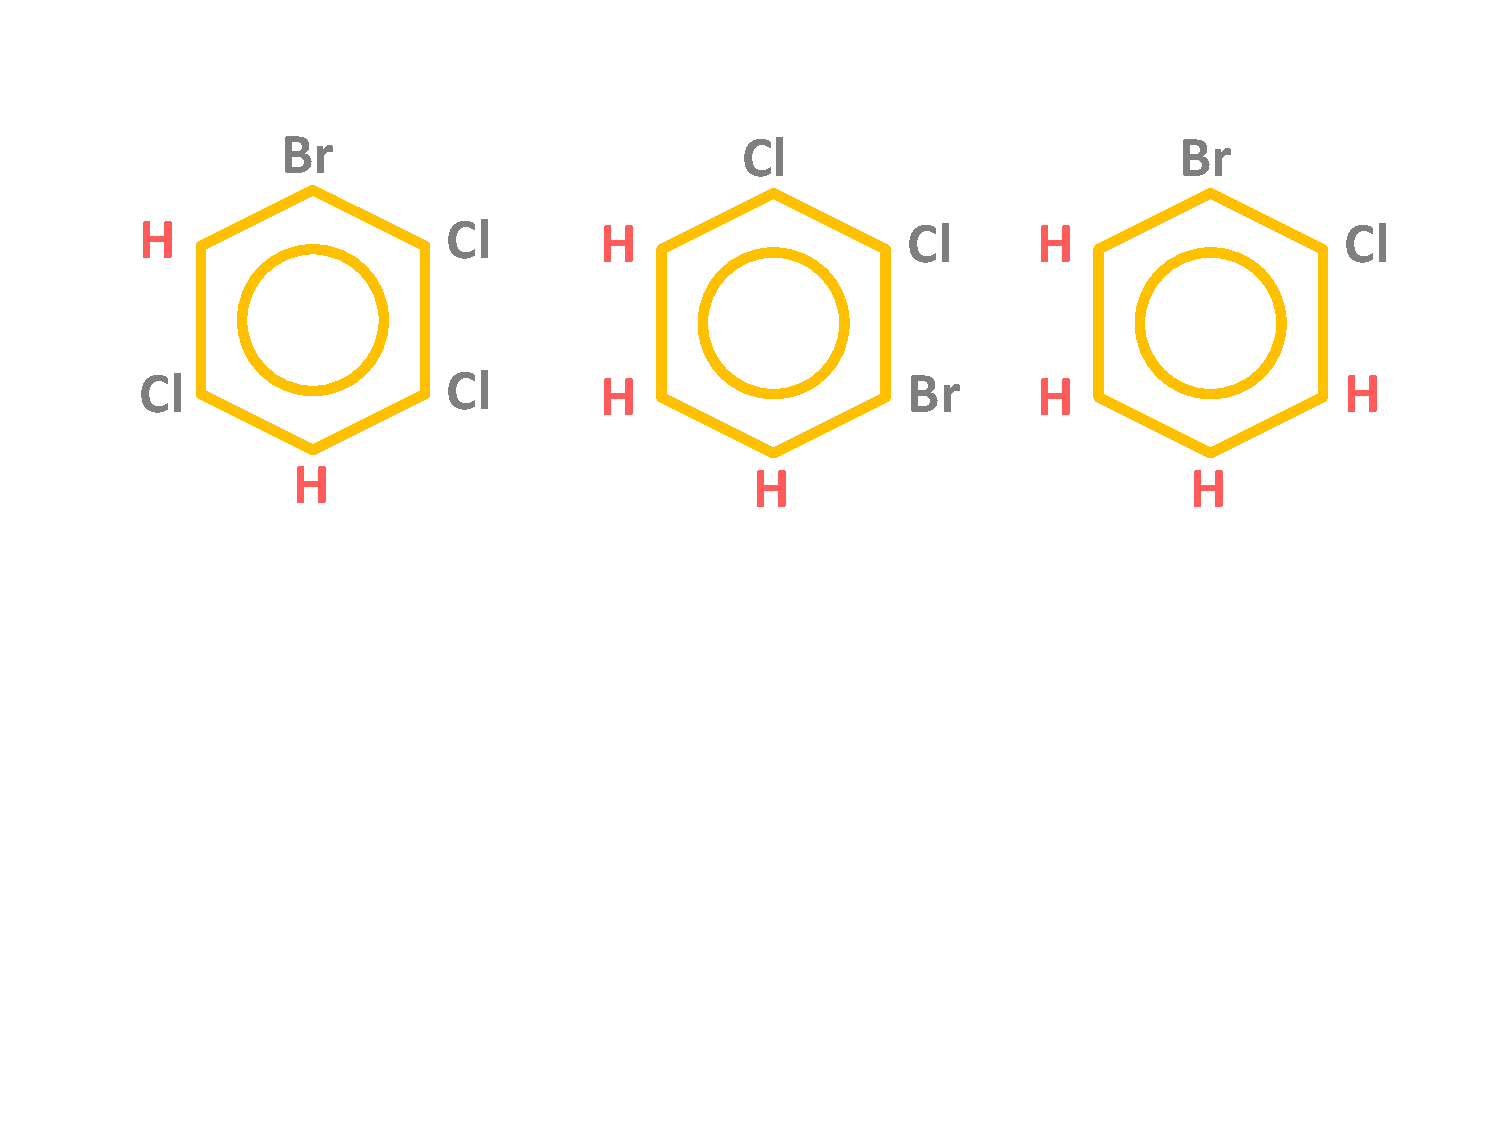
\includegraphics[width= 0.8\columnwidth]{figures/lqsample.pdf}
              \caption{2, 3, 4 qubit的液晶样品结构。苯环上的$^1$H被用作qubit。
              }
              \label{lqsample}
            \end{center}
\end{figure}

NMR量子计算的第一步是PPS制备,液晶样品也不例外。除了前面提到过的液体NMR中各种PPS制备方法,针对液晶体系特殊的哈密顿量形式
又有一些新的技巧,比如线选脉冲饱和能级\cite{lq3},制备PPS对\cite{lq4,lq5,lq6}等。这些方法都有着或多或少的局限性。
借助于GRAPE脉冲,我们设计了基于GRAPE搜索的PPS制备方法,其基本思路为
\begin{equation}\label{aaa}
\sum_i I^i_z \rightarrow U\rightarrow Gz \rightarrow\rho_{pps}.
\end{equation}
可以看出,我们只用了一个幺正操作和一个梯度场,就可使实现PPS。该方法的核心在于如何找到这样一个操作$U$,并把它写成脉冲的形式。

首先我们把$U$分割,即
\begin{equation}\label{aaa}
U = U_N U_{N-1}\cdots U_1,
\end{equation}
其中
\begin{equation}\label{aaa}
U_j = e^{-i\Delta t ((H_{int} + \sum_{k=1}^mu_k(j)H_{ext})}.
\end{equation}

对于PPS,我们设其理论形式为
\begin{equation}\label{aaa}
\rho_{th} = \left \vert 0\ldots 0 \right \rangle \left \langle 0\ldots 0 \right \vert - \frac{I}{2^n},
\end{equation}
$n$为qubit的数目。在施加了GRAPE脉冲及梯度场后,我们的末态为
\begin{equation}\label{aaa}
\rho_{exp} = Gz(U \rho_{in} U^{\dagger}).
\end{equation}

为了衡量$\rho_{exp} $和$\rho_{th}$之间的相似程度,我们采用了式\ref{correlation}定义的相关性
\begin{equation}\label{correlation}
C = \frac{Tr(\rho_{exp} \rho_{th})}{\sqrt{Tr(\rho_{exp}^2)Tr(\rho_{th}^2)}}.
\end{equation}

假设
\begin{equation}\label{aaa}
U = U_B U_{j} U_A,
\end{equation}
且$U_A = U_{j-1}\cdots U_1$,$U_B = U_N\cdots U_{j+1}$。我们对幅度因子$u_j$进行一个微扰$\Delta u_j$后,可以得到相关性$C$感受到的微扰$\Delta C_j$,然后我们就可以进行新的梯度修正
\begin{equation}\label{aaa}
u_j \rightarrow u_j + \epsilon \frac{\Delta C_j}{\Delta u_j}.
\end{equation}
这个思路和GRAPE脉冲的思想非常类似,而通过循环搜索,我们可以得到保真度很高的GRAPE脉冲。
例如,在4 qubit液晶体系,我们可以得到2000$\mu s$,分为400小片,保真度为0.97的GRAPE脉冲。

在完成了PPS制备后,我们要考虑如何有效地在液晶体系上进行幺正演化。注意到液晶的哈密顿量不是对角的,
一个很自然的想法是把它进行对角化
\begin{eqnarray}\label{aaa}
U^{\dagger} H U = H_D, \nonumber \\
UH_DU^{\dagger}  = H.
\end{eqnarray}
其中$H_D$指的是对角化后的哈密顿量,对应于液体NMR中的形式。必须提到矩阵对角化在经典计算上本身是一个多项式难的问题,所以这一步其实仅在低量子位有效。而哈密顿量对角化的量子算法可以参见文献\cite{lq7}。

在对角化之后,我们发现经过这个幺正变换$U$后液晶体系的读出和液体居然是一样的,因为
\begin{eqnarray}
&&Tr(e^{-iH_Dt}R\rho R^{\dagger}e^{iH_Dt}\cdot F^{+}) \nonumber \\
&=&Tr(Ue^{-iH_Dt}U^{\dagger}\cdot  URU^{\dagger} \cdot  U \rho U^{\dagger}  \cdot  U  R^{\dagger} U^{\dagger} \cdot  U e^{iH_Dt} U^{\dagger}  \cdot  U  F^{+} U^{\dagger}) \nonumber \\
&=&Tr(e^{-iHt}\cdot  URU^{\dagger} \cdot  U \rho U^{\dagger}  \cdot  U  R^{\dagger} U^{\dagger} \cdot  e^{iHt} \cdot  F'^{+} ).
\end{eqnarray}
那么,我们只要把液体NMR中的初态$\rho$和幺正操作$R$转化到液晶体系中就可以了,需要的仅仅是把初态变为
$U \rho U^{\dagger}$,操作变为$ URU^{\dagger}$。

液晶NMR的读出和逻辑操作类似,只要把用于液体的重构序列进行一个幺正变换$U$即可,而其测量方式和液体NMR完全相同。

最后整理下液晶NMR量子计算的步骤。

$\bullet$ 测量液晶样品的热平衡谱,并解谱得到哈密顿量形式。

$\bullet$ 求解其本征值和本征态,并进行对角化操作,得到用来对角化的操作$U$及对角化后的哈密顿量$H_D$。

$\bullet$  假定量子计算实验是在液体NMR样品$H_D$中完成的,并设计在该样品完成时如何进行初态制备,逻辑操作,结果读出等。

$\bullet$ 把$H_D$中所有的操作前面都施加幺正变换$U$,再移植到液晶样品中。由于$U$的形式一般不规律,最好是通过SMP或是GRAPE脉冲算出。

$\bullet$  液晶中所有的测量读出脉冲也和液体类似,只不过加上幺正变换$U$。

为了证明以上思路的可行性,接下来我们将以一个4 qubit液晶NMR实验为例具体讲解。

\subsection{利用4 qubit液晶样品绝热分解143}

前面已经提到,最能代表量子计算优越性的算法是Shor的大数分解算法\cite{Shor},但实验上想验证Shor算法是非常困难的。
最早的实验是2000年利用7 qubit
NMR样品分解了15\cite{shor15},这也是NMR量子计算早期的代表工作。后来,我们组提出了基于绝热的量子分解算法,需要的资源更少,复杂度也更低,并在3 qubit样品上成功分解了21\cite{shor21},光学体系也相继分解了15\cite{optshor15}。最近,我们改进了自己提出的绝热分解算法,设计了4 qubit分解143的实验方案,并在4 qubit液晶NMR样品上完成了这一实验\cite{shor143}。本节我们就将主要介绍该实验过程。

首先简要介绍一下绝热量子计算(adiabatic quantum computing, AQC)\cite{aqc1}。在AQC的框架中,量子体系首先被制备到初始哈密顿量$H_0$的基态,而量子计算任务的答案则蕴含在最终哈密顿量$H_p$的基态里。
在计算过程冲,含时的哈密顿量非常缓慢地从$H_0$变化到$H_p$,保证量子体系一直处于当前哈密顿量的基态上。最后,通过测量末态,也就是$H_p$的基态,
我们就可以得到问题的解。最简单的哈密顿量变化形式是如下插值
\begin{equation}\label{aaa}
H(t) = [1-s(t)]H_0+s(t)H_p,
\end{equation}
其中$s(t)$从0缓慢地变化到1。AQC比较适合的是求解最优化问题,因为很多最优的解都是蕴含在哈密顿量的基态中。

对于大数的分解问题,我们可以用$N = p\times q$给出,$p$和$q$是$N$的两个质因子。设计AQC的核心在于如何把这样一个等式转化为最优化问题,最直接的想法是通过
等式$N - pq = 0$来构造函数$f(x,y) =(N - xy)^2$。$f(p,q)=0$肯定是这个函数的最小值,也是其最优解。那么,末态哈密顿量就可以选择为
\begin{equation}\label{interpo}
H_p = (N - \hat{x}\times\hat{y})^2,
\end{equation}
其中,$\hat{x}$用$\sum_{i = 0}^{n-1}2^i(\frac{1-\sigma_z^i}{2})$来构造,且$n$为$x$转化为二进制时的比特数。算子$\hat{y}$也可以类似构造。那么,
$H_p$的基态能量就为0,代表$N = p\times q$。NMR上进行的21分解的实验就是用这种构造方式完成的\cite{shor21}。

在上述方案中,末态哈密顿量的能谱宽度是和要分解的数$N$成线性关系的,因此当$N$很大时,实验上很难找到如此具有如此大
能谱宽度的哈密顿量。后来,Schaller和 Sch\"{u}tzhold\cite{aqc2,aqc3}利用求解线性方程组的方法优化了这个问题。在143分解中,我们把$N = p\times q$转化为二进制形式的乘法,并用图\ref{linearset}中所示的二进制乘法表列出一系列的方程,构成线性方程组。可以看到,
目标问题把确定质因子$p$和$q$转化为确定二进制数$p_1,p_2$和$q_1,q_2$,然后把二进制数$1p_2p_11$和$1q_2q_11$转化为十进制即可。

\begin{figure}[htbp]
            \begin{center}
              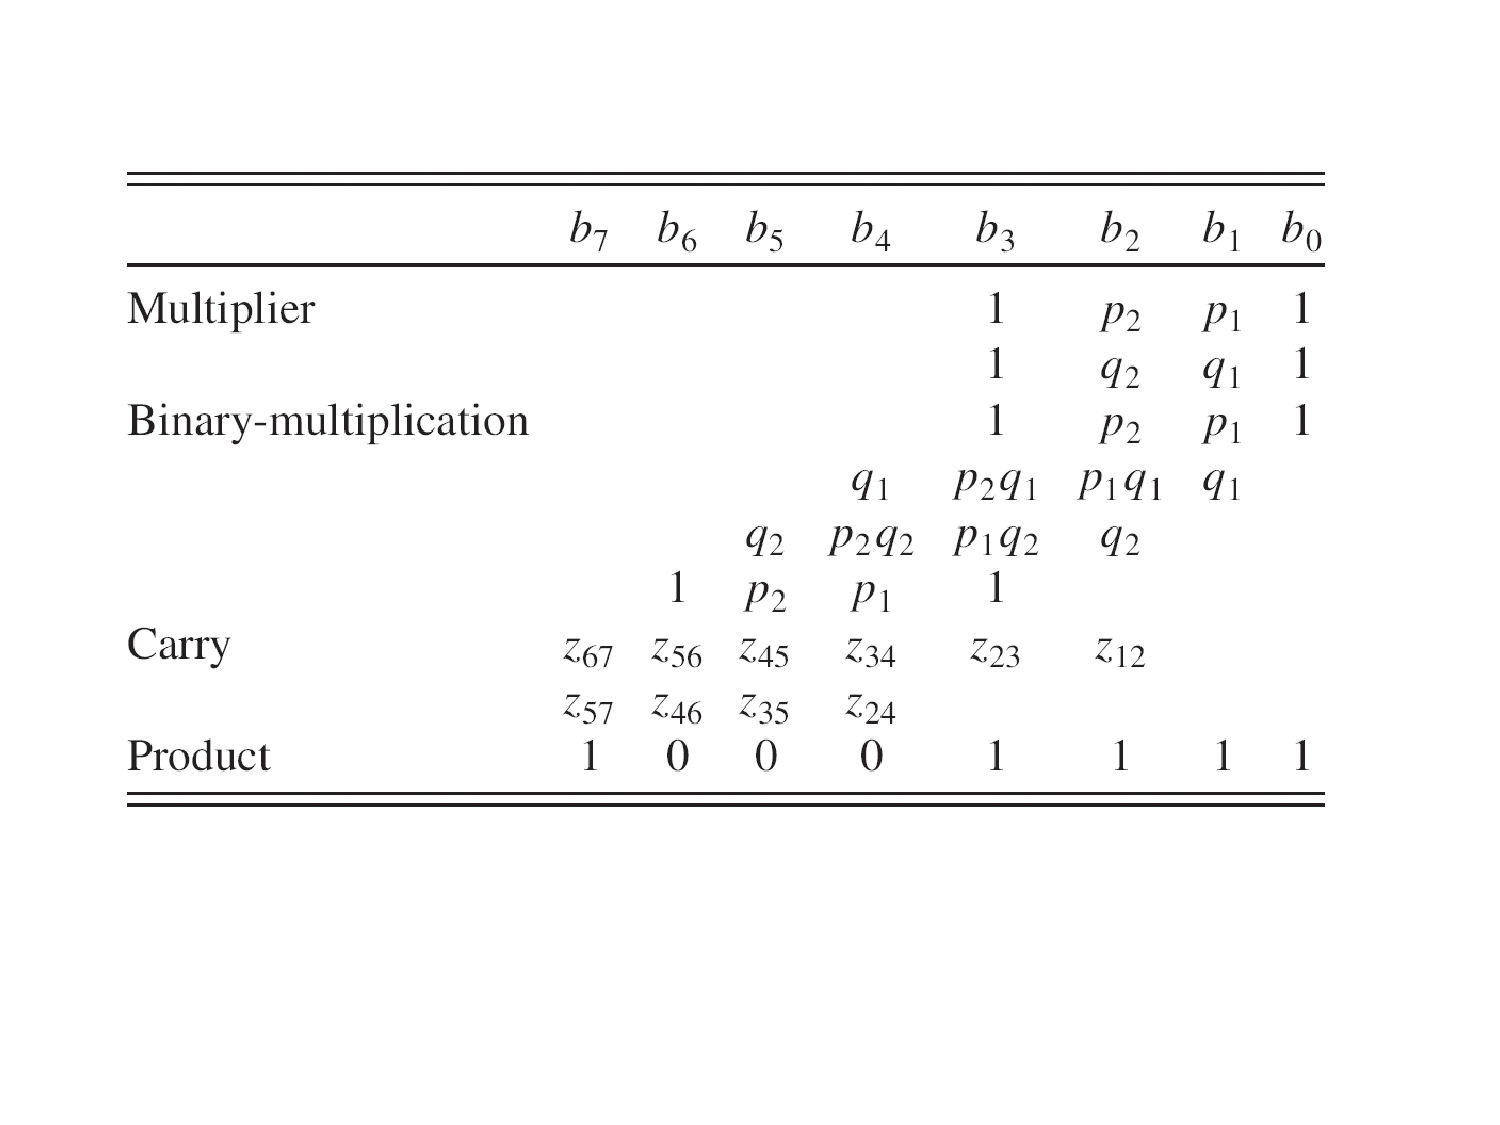
\includegraphics[width= 0.8\columnwidth]{figures/linearset.pdf}
              \caption{$N = 143$分解中用到的二进制乘法表。$N = p\times q$中的所有数值都被转化为了二进制,然后利用这个乘法结构可以列出一个线性方程组。
              }
              \label{linearset}
            \end{center}
\end{figure}

通过约束条件化简该线性方程组后(具体过程请参见文章\cite{shor143}),我们得到目标,也就是末态哈密顿量的形式为
\begin{eqnarray}
H_p &=& 5-3 \hat{p}_1-\hat{p}_2-\hat{q}_1+2 \hat{p}_1 \hat{q}_1-3 \hat{p}_2 \hat{q}_1\nonumber\\
&+&2 \hat{p}_1 \hat{p}_2 \hat{q}_1-3 \hat{q}_2+\hat{p}_1
\hat{q}_2+2\hat{p}_2 \hat{q}_2+2 \hat{p}_2 \hat{q}_1
\hat{q}_2,\label{hp}
\end{eqnarray}
其中$\hat{p}$ 和 $\hat{q}$被映射到了qubit空间$\hat{p}_1=\frac{1-\sigma_z^1}{2},
\hat{p}_2=\frac{1-\sigma_z^2}{2}, \hat{q}_1=\frac{1-\sigma_z^3}{2}$,$ \hat{q}_2=\frac{1-\sigma_z^4}{2} $。

绝热演化的初始哈密顿量可以选择容易制备其初态的哈密顿量形式,例如这里选择的是
\begin{equation}\label{aaa}
H_0=g(\sigma_{x}^{1}+\sigma_{x}^{2}+\cdots+\sigma_{x}^{n}).
\end{equation}
该哈密顿量的基态形式为所有计算基矢的叠加,即
\begin{equation}\label{aaa}
\left \vert \psi_i \right \rangle=\left(
\frac{|0\rangle-|1\rangle}{\sqrt{2}} \right)^{\otimes n}.
\end{equation}
在计算过程中,首先我们把量子体系制备到$H_0$的基态$|\psi_i\rangle$上,然后依据插值公式\ref{interpo}把$H_0$
缓慢地变化到$H_p$,绝热定理保证系统始终处于当前哈密顿量的基态上。最后,通过测量末态的形式,我们可以得到
二进制数$p_1,p_2$和$q_1,q_2$,从而得到
143分解问题的解。该过程的数值模拟可以参加图\ref{143sim}(a)。

\begin{figure}[htbp]
            \begin{center}
              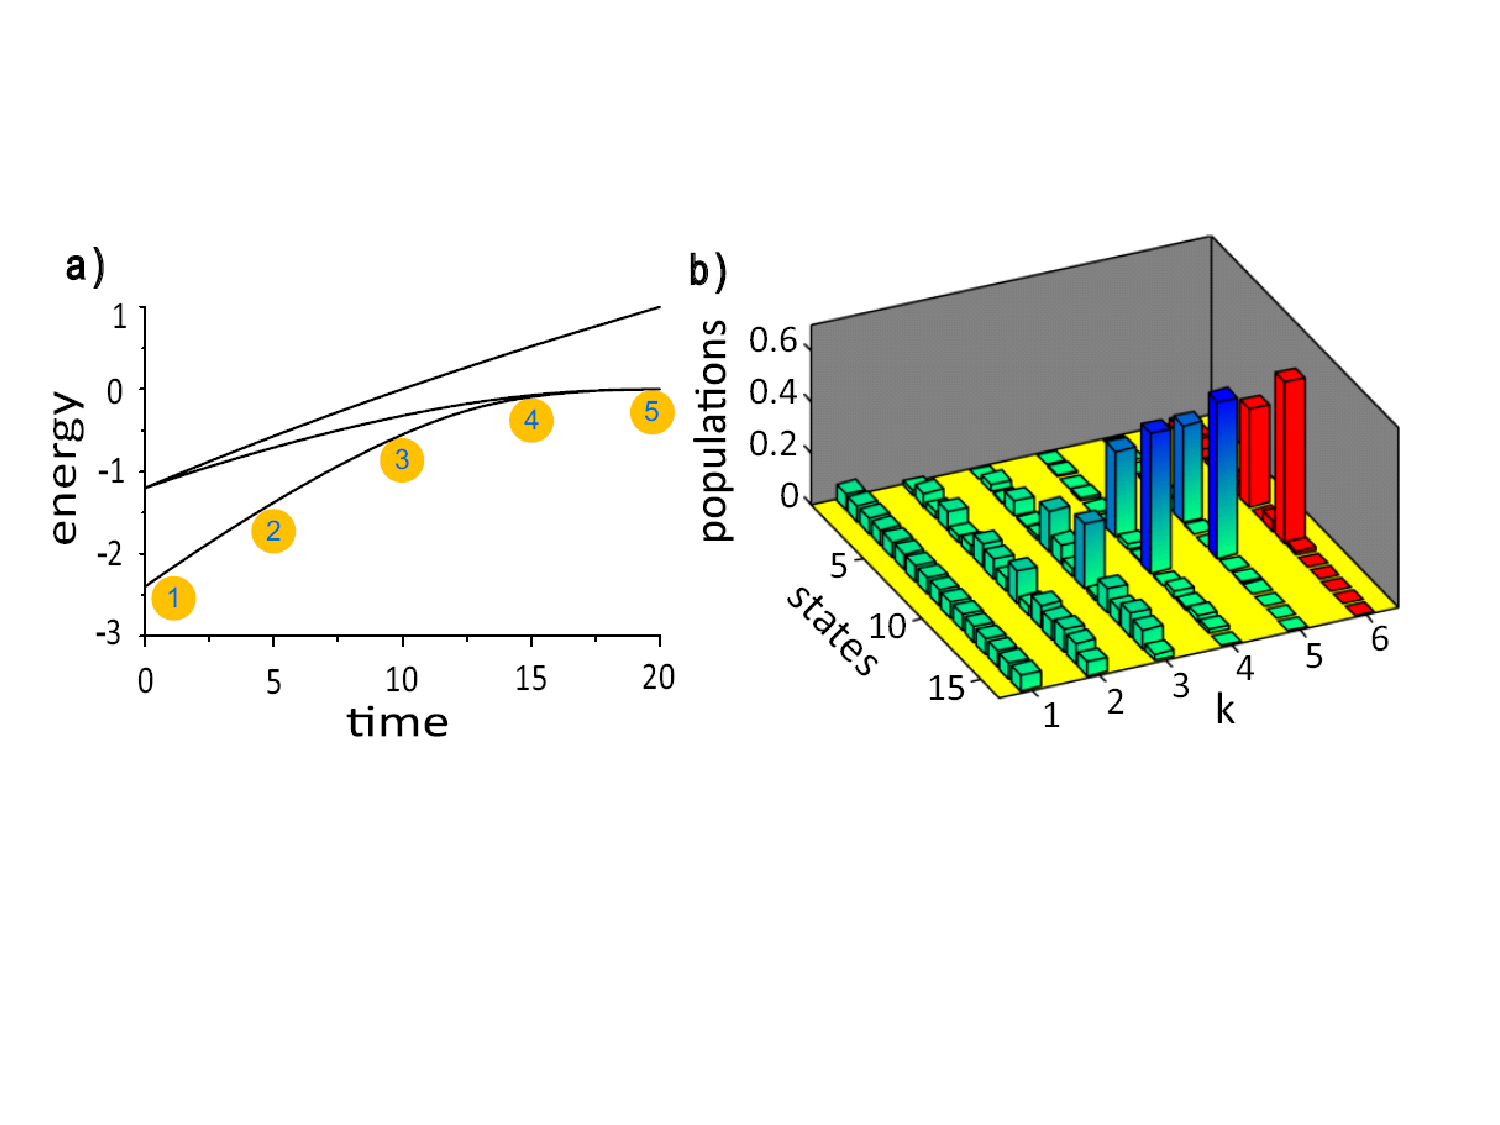
\includegraphics[width= 0.8\columnwidth]{figures/143sim.pdf}
              \caption{(a) 143分解中,最低的三个能级变化的示意图。初始哈密顿量中的$g$因子设为0.6。(b) $k = 1-5$对应图(a)中5个点的布居度分布。$k = 6$则是实验上得到的末态的布居度分布。可以看到,最终所有的布居度几乎都处于
              $\left \vert 0110 \right \rangle \left \langle 0110 \right \vert$和$\left \vert 1001 \right \rangle \left \langle 1001 \right \vert$上,表示143分解的结果为$p =11,q=13$或者$p = 13,q=11$。}
              \label{143sim}
            \end{center}
\end{figure}

在实验上,我们选择了4 qubit液晶样品1-bromo-2-dichloro-benzene(图\ref{143sample}(a))溶于ZLI1132作为量子体系。样品中的四个$^1$H
核自旋作为四个qubit,其哈密顿量形式为
\begin{equation}
 \mathcal{H} = 2\pi\sum_i \nu_i
 I_z^i+2\pi\sum_{i,j,i<j}J_{ij}I_z^iI_z^j
 +2\pi\sum_{i,j,i<j}D_{ij}(2I_z^iI_z^j-I_x^iI_x^j-I_y^iI_y^j).
\end{equation}
通过热平衡态(图\ref{143sample}(b))的解谱,我们得到了哈密顿量中的所有参数为化学位移$\nu_1=2264.8$Hz, $\nu_2=2190.4$Hz,
$\nu_3=2127.3$Hz, $\nu_4=2113.5$Hz,偶极耦合大小$D_{12}=-706.6 $Hz, $D_{13}=-214.0$Hz, $D_{14}= -1166.5$Hz,
$D_{23}=-1553.8$Hz, $D_{24}=-149.8$Hz, $D_{34}=  -95.5$Hz,$J$耦合大小$J_{12}=0$Hz, $J_{13}=1.4$Hz, $J_{14}=8$Hz,
$J_{23}=8$Hz, $J_{24}=1.4$Hz, $J_{34}=8$Hz。得到了这些参数后,我们还对热平衡态中的各条谱线进行了相应的能级跃迁标记(图\ref{143sample}(c))。

\begin{figure}[htbp]
            \begin{center}
              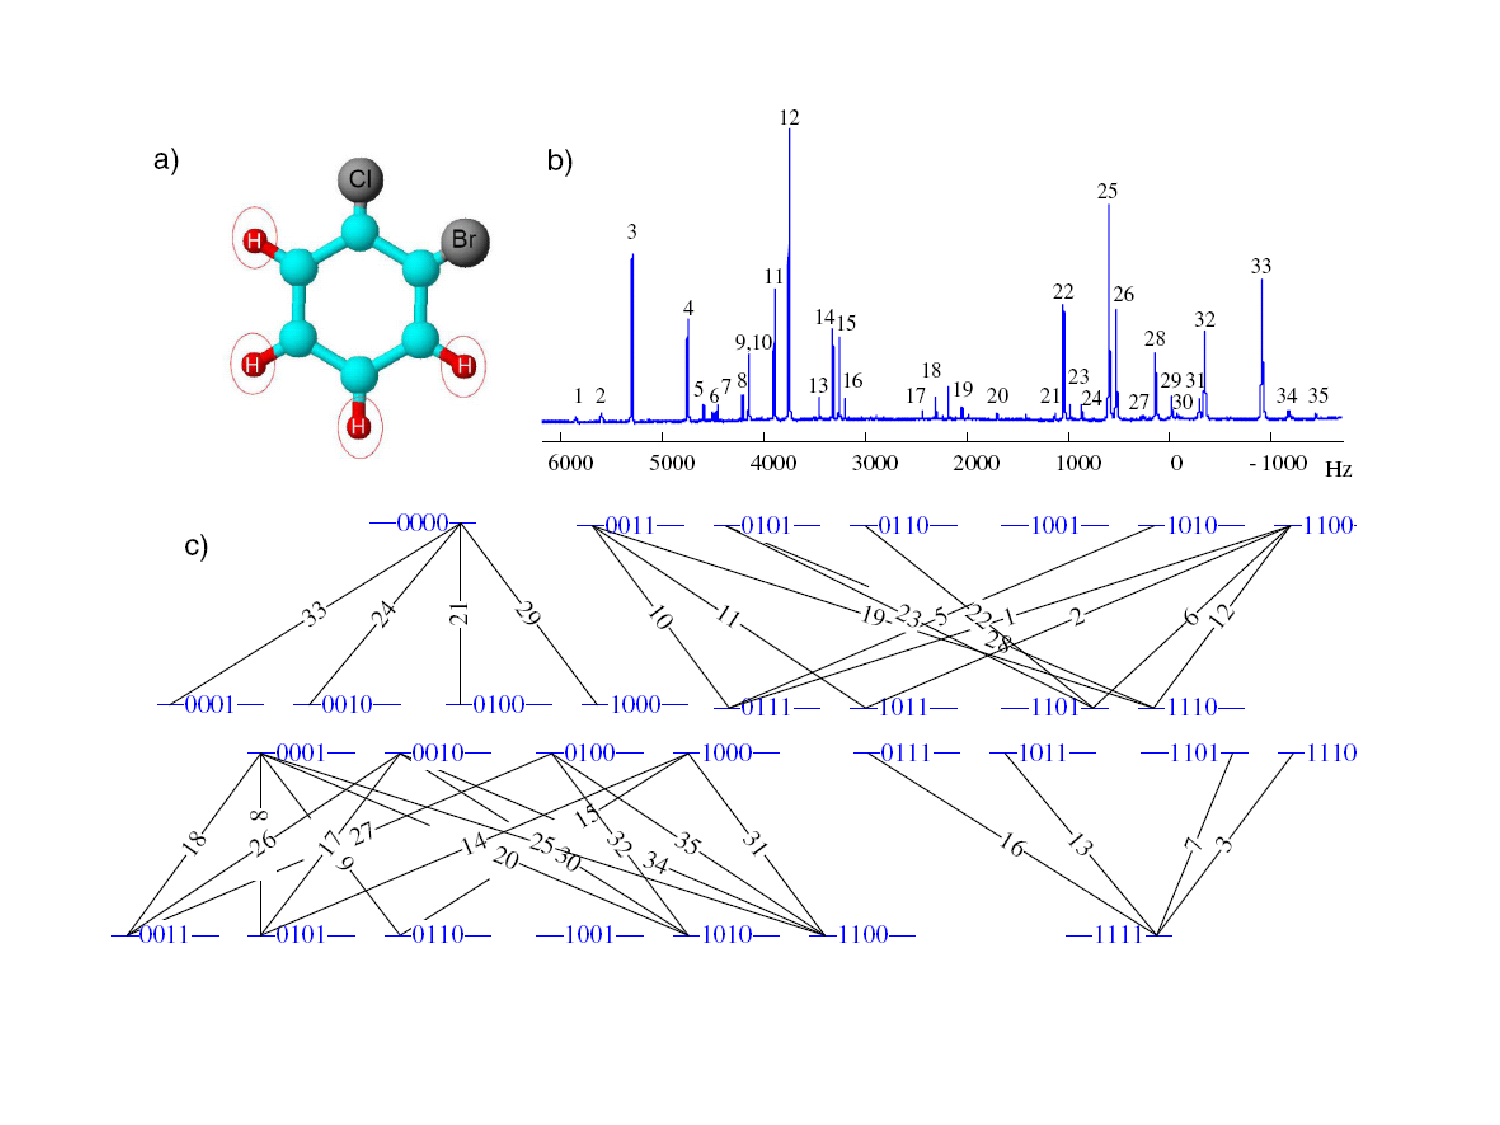
\includegraphics[width= 0.8\columnwidth]{figures/143sample.pdf}
              \caption{143分解实验中用到的4 qubit 液晶NMR样品。(a) 1-bromo-2-dichloro-benzene的分子结构。(b) 热平衡态的NMR谱线。跃迁的序号是依据谱线频率的降序排列的。(c)与(b)图相关的能级跃迁图。}
              \label{143sample}
            \end{center}
\end{figure}

实验的第一步是PPS制备。一般来说,为了构造PPS中的四体关联,空间平均法需要很多脉冲和梯度场的组合。而在143分解的实验中,我们利用
GRAPE算法计算了一个幺正算子,并把它打包成了GRAPE脉冲。在热平衡态上施加完这个GRAPE脉冲以及梯度场之后,我们就成功制备了PPS。
具体来说,实验上热平衡态的形式是$\rho_{eq}=\sum_{i=1}^4 \gamma_i I_z^i$,其中$\gamma_i$是核自旋的旋磁比。对于同种核自旋来说,$\gamma$的值是可以忽略的。

理论上我们要制备的PPS为
\begin{equation}\label{aaa}
\rho_{theo}=-\frac{1}{16}\mathbb{{I}}+\left\vert 0000 \right\rangle \left\langle0000\right\vert,
\end{equation}
其中${\mathbb{{I}}}$是 $16\times16$ 的单位阵。首先,我们猜测一个算子$U_0$,并计算当前PPS理论形式$\rho_{theo}$与实验结果
\begin{equation}\label{aaa}
\rho_{fin}=Gz(U_0\rho_{eq}U_0^{\dagger})
\end{equation}
之间的保真度$F$。如果$F$高于我们的预设值(在本实验中$F$设为0.99),我们就把$U_0$打包成一个GRAPE脉冲。否则,我们将在GRAPE算法的指导下,重复上面的过程计算一个新的$U_0$,直到
满足条件的$U_{pps}$找到。对于本实验中的液晶样品来说,我们寻找到执行$U_{pps}$的GRAPE脉冲的脉宽为7ms,250小片。在加完$U_{pps}$及梯度场后,如果忽略掉梯度场不能消除的但几乎为0的零量子相干,我们得到的
PPS的对角元为[1.512, -0.098,-0.120,-0.109,-0.100,-0.072,-0.112,-0.098,-0.106,-0.136,-0.083,0.097,-0.052,-0.112,-0.081,-0.136]。在扣除单位阵背景后,这个态和$\left\vert 0000 \right\rangle$之间的保真度超过0.99,而相比于热平衡态,我们制备的PPS信号损失了$76.8\%$。在制备了PPS后加了一个小角度观测的NMR谱参见图\ref{143result}(a)。

\begin{figure}[htbp]
            \begin{center}
              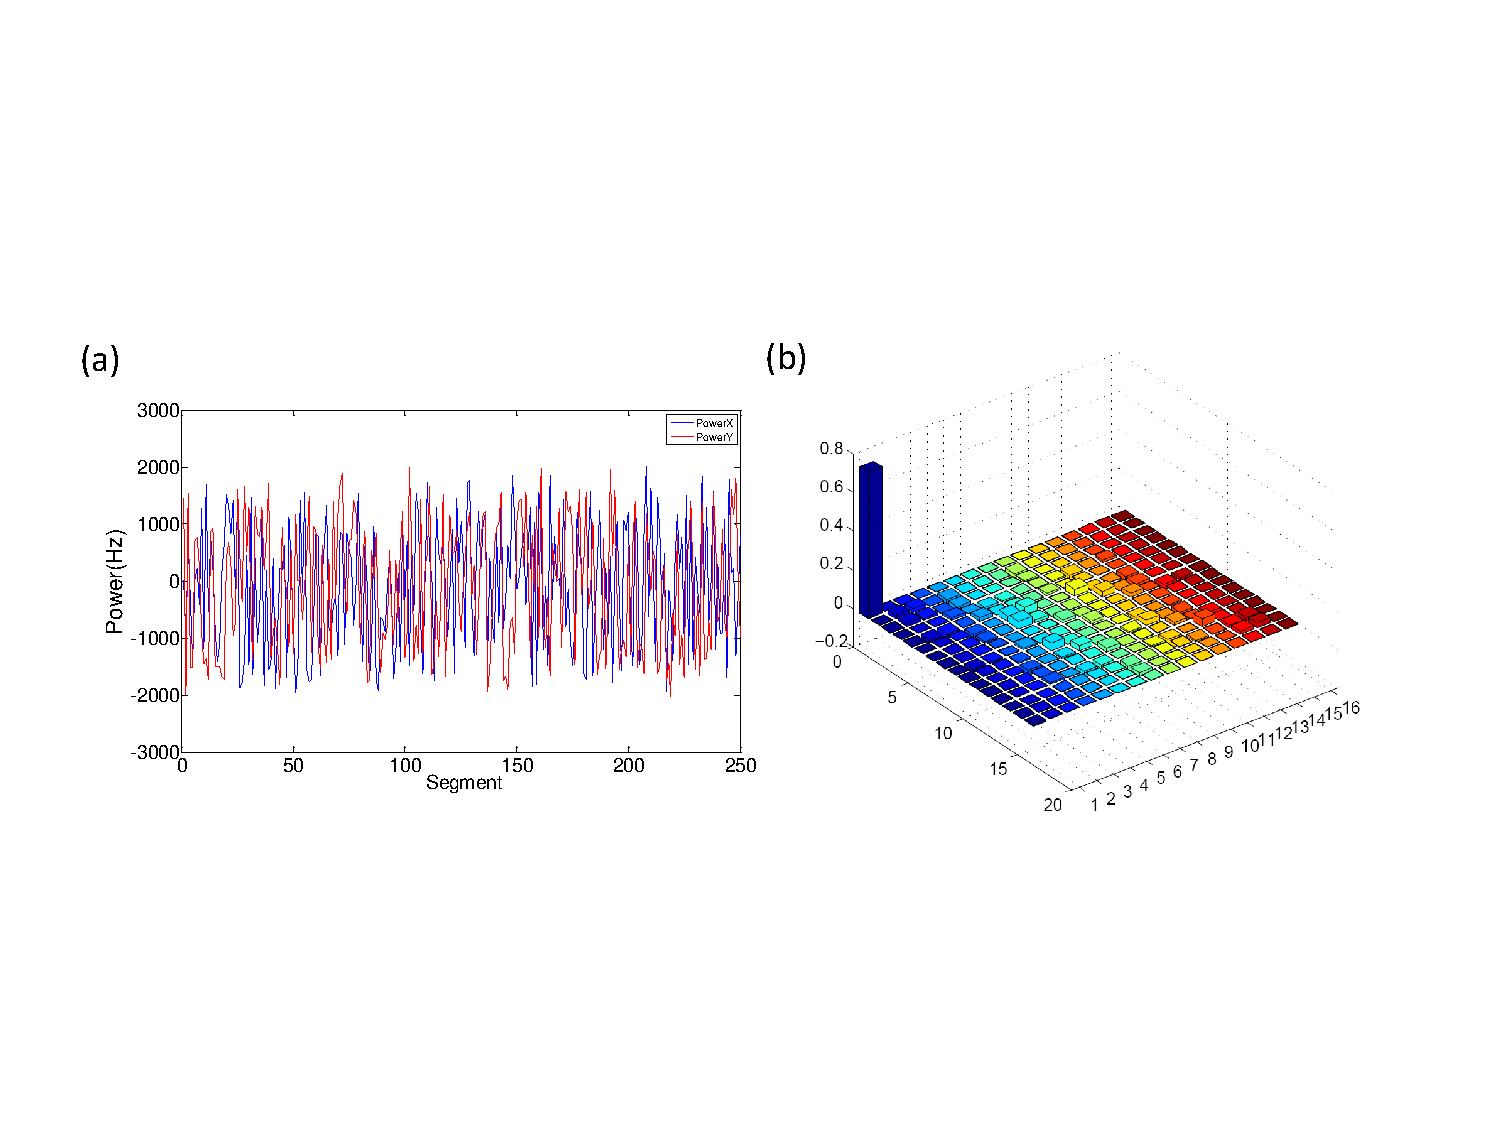
\includegraphics[width= 0.8\columnwidth]{figures/143pps.pdf}
              \caption{(a) 143分解中制备PPS用到的GRAPE脉冲。蓝线和红线分别代表加在$\hat{x}$方向和$\hat{y}$方向的射频场强度的变化。(b)数值模拟的制备PPS的结果,这里只给出了实部。可以看出,几乎所有的信号都集中在布居度$\left\vert 0000 \right\rangle \left\langle 0000 \right\vert$上,而这条峰一般被用作NMR量子计算测量的基准。}
              \label{143pps}
            \end{center}
\end{figure}

143分解的核心是通过绝热量子计算实现的。首先,我们在制备的PPS$\left\vert 0000 \right\rangle$加一个$\hat{y}$方向的$\pi/2$硬脉冲,同时翻转所有的qubit。这样,系统就被制备到$H_0$的基态,也就是
$|-\rangle^{\otimes4}$
($|-\rangle=(|0\rangle-|1\rangle)/\sqrt{2}$)。绝热演化过程我们一共分了$M$步\cite{aqc4,aqc5},且插值方式选择为线性的$s(t)=t/T$。
因此,每一小步的绝热演化为$U_{m}=e^{-iH(m)\tau }$ ,其中$\tau=T/M$为每一步的演化时间,而
\begin{equation}\label{aaa}
H_m =(1-\frac{m}{M})H_0+\frac{m}{M}H_p,
\end{equation}
为当前绝热演化的哈密顿量。总的演化算子就可以写成$U_{ad}=\prod_{m=1}^{M}U_{m}$,且当$T,M\rightarrow\infty$绝热条件就会满足。
实验中我们选择的参数为$g=0.6,
M=20$,$T=20$。数值模拟的结果发现系统最终处于$H_p$基态的概率为$98.9\%$。而在实验上,我们把每五步绝热演化的幺正算子计算成一个
GRAPE脉冲,每个GRAPE脉冲的时间为15ms,且保真度超过0.99,因此总的演化时间为60ms。

最后,我们需要对末态密度矩阵$\rho_{fin}$的所有对角项进行测量,采用的是我以前提出的密度矩阵对角化方法\cite{rw1}。在4 qubit液晶中,我们采用了32个读出脉冲来测量所有的布居度,每个读出脉冲都打包成了20ms的GRAPE脉冲。结合归一化条件$\sum_{i=1}^{16}P(i)=1$,我们可以得到末态$\rho_{fin}$
中所有对角元的值。由于本实验中演化时间为60ms,而$T_2^{*}$也只有102ms,所以我们利用$e^{-T_{tot}/T_2^{*}}$补偿了退相干的影响,实验结果显示在
图\ref{143sim}(b)中的$k=6$步。可以看出,在补偿了退相干后,实验结果$(k=6)$和理论预期$(k=5)$是非常吻合的。

另一方面,为了从NMR的实验谱线上给出更容易理解的结果,我们在得到了末态$\rho_{fin}$后,在第二和第三个qubit上加一个$\pi$脉冲,然后在加一个梯度场,即
\begin{eqnarray}
\rho_{out} = Gz(R_y^{2,3}(\pi)\rho_{fin}R_y^{2,3}(\pi)^{\dagger}).
\end{eqnarray}
然后再利用小角度(3$^{\circ}$)进行观测。这样做的好处是我们把实验结果从$\left\vert 0110
\right\rangle \left\langle 0110 \right\vert$和$\left\vert 1001
\right\rangle \left\langle 1001 \right\vert$转化到了$\left\vert 0000
\right\rangle \left\langle 0000 \right\vert$ 和 $\left\vert 1111
\right\rangle \left\langle 1111 \right\vert$。在液晶样品中,由于哈密顿量的本征态不再是Zeeman直积态,而是它们的线性组合,因此传统的$\pi/2$观测不再是一条谱线。
但是,$\left\vert 0000
\right\rangle$ 和 $\left\vert 1111
\right\rangle$则依然是哈密顿量的本质态,虽然它们的 $\pi/2$观测也不是单一的吸收峰,但小角度激发的结果主要只包含一根吸收峰。也就是说,在进行了以上变换且用小角度观测后,我们得到的实验结果应该主要含有两条谱线,一条位于$\rho_{0000}$
的小角度观测处,另一条位于$\rho_{1111}$的小角度观测处。图\ref{143result}直观地给出了我们的实验结果(蓝线),和模拟结果(红线)几乎完全一样,说明我们找到143的质因子为11和13或者13和11。

\begin{figure}[htbp]
            \begin{center}
              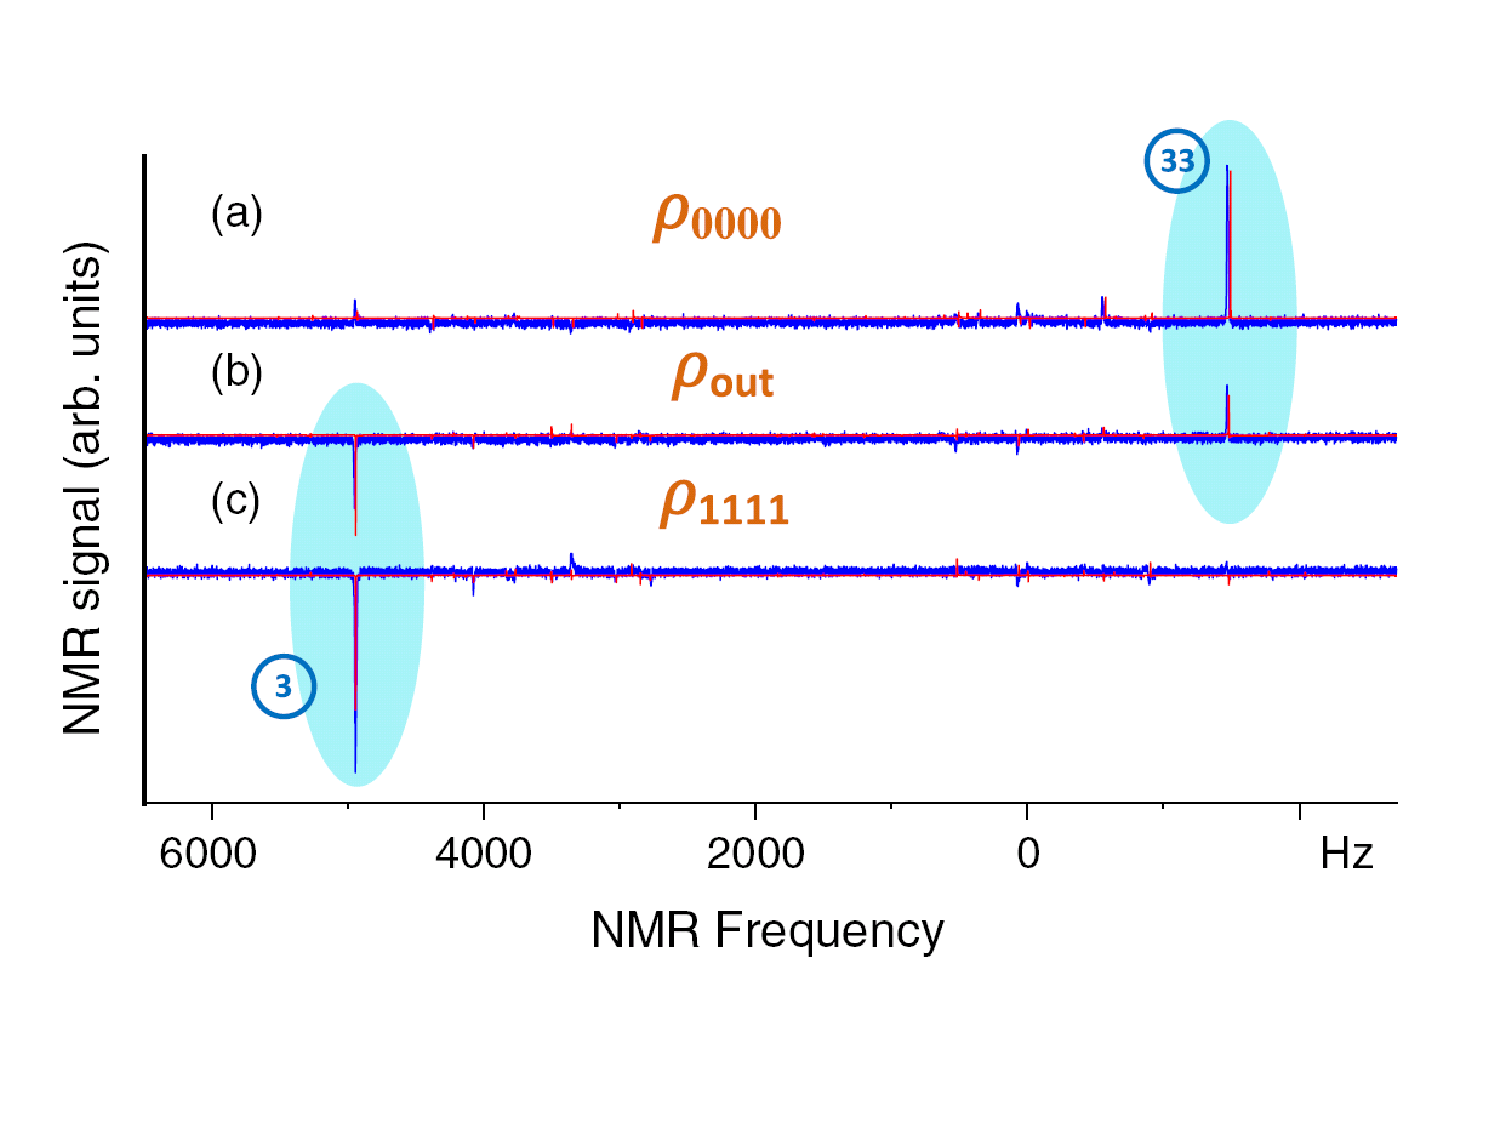
\includegraphics[width= 0.8\columnwidth]{figures/143result.pdf}
              \caption{(a) NMR实验上小角度观测的PPS谱线及输出态$\rho_{out}$的谱线。蓝线为实验结果,而红线为理论结果。谱线上标的No. 33 和No. 3对应于图\ref{143sample}(b)中的序号。}
              \label{143result}
            \end{center}
\end{figure}

总结来说,我们利用改进的绝热算法在实验上成功分解了143。由于利用的是4 qubit液晶NMR样品,所以从哈密顿量解谱,初态制备,绝热演化到测量读出等很多方面都是依靠新的设计。143分解的成功实现也进一步验证了
这些实验思路都是正确的。目前为止,143是量子计算实验上分解的最大的数,也是唯一一个超过100的数字。

本节的工作已发表在Phys. Rev. Lett. 108, 130501 (2012)\cite{shor143}上。



\section{小结}

在本章中,我们简要叙述了NMR量子计算的理论框架,并给出了一些实验上的技术及处理技巧。以目前的实验进展来看,
液体NMR量子计算已经发展的非常成熟,并且会对NMR本身以及其他体系产生很重要的推动作用。比如,动力学解耦(dynamical decoupling)技术已经在很多非量子计算的实验中得到了应用,而GRAPE脉冲技术甚至移植到了其他体系,例如ESR,离子阱中等。但我们也要认识到,虽然
NMR的优势很大,它也有很大的局限性,主要集中在以下两点:

首先,NMR量子计算是系综量子计算,我们已经说过大概要$10^{18}$个分子才能探测,赝纯态的“赝”字也正表示NMR还不能制备出真正的纯态。
不仅不能制备真正的纯态,量子计算中的另一个重要资源-纠缠也是不可能实现的。基于系综的这些问题也使得NMR量子计算经常被很多学者诟病,认为它并不是
实现了真正的量子计算。尽管如此,一些演示性的实验确实很适合用NMR平台,而量子无序(quantum discord)的提出为NMR量子计算指明了另一个方向,因为NMR中确实是存在量子无序的。

第二,NMR的可扩展性并不是很好。当自旋数目增加时,整个频率空间由于有$n2^{n-1}$条共振谱线而会变得非常拥挤,非常难于寻址,另外,自旋数目增加后选择脉冲的时间会
变得很长,导致逻辑操作的时间大大延长,非常不利用量子计算任务。

虽然有这些弱点,但NMR依然是量子计算领域不可或缺的实验方向,从中产生的很多新技术。新思路,新方法,以及通过它验证的众多量子计算理论,都大大保证了NMR量子计算的生命力,本篇论文的后半
部分的实验工作都是基于NMR的,通过它们的介绍我们也可以看出NMR上还是能做出一些非常漂亮的工作。

最后,比较推荐的关于NMR的参考书有两本:

$\bullet$ Freeman的《Spin Choreography》\cite{pps7}。这本书非常系统全面,且以通俗易懂的语言回顾了高分辨的NMR技术及自旋动力学。这本书在科大东区的外文图书库存有一本。

$\bullet$ NMR领域的第一个诺贝尔奖得主Ernst写的经典著作《Principles of Nuclear Magnetic Resonance
in One and Two Dimensions》\cite{ernst}。这本书有中译本,而且其权威性不容置疑,但相对上一本要难懂一些。不过对于了解基本的NMR技术,中文可能更适合一些。

据我所知,目前并没有NMR量子计算的教科书,但有一些比较适合的综述性文献\cite{nmrtext1,nmrtext2,nmrtext3,nmrtext4}。尤其推荐的是 Vandersypen和Chuang撰写的《NMR techniques for quantum control and computation》\cite{nmrtext3},对于NMR量子计算的介绍非常详尽,而两人也是该领域的著名学者。另外就是Jones的《Quantum computing with NMR》\cite{nmrtext4},一共有500余篇关于NMR量子计算的参考文献(截止2010年),可以作为很有用的工具书使用。

